% The document class supplies options to control rendering of some standard
% features in the result.  The goal is for uniform style, so some attention 
% to detail is *vital* with all fields.  Each field (i.e., text inside the
% curly braces below, so the MEng text inside {MEng} for instance) should 
% take into account the following:
%
% - author name       should be formatted as "FirstName LastName"
%   (not "Initial LastName" for example),
% - supervisor name   should be formatted as "Title FirstName LastName"
%   (where Title is "Dr." or "Prof." for example),
% - degree programme  should be "BSc", "MEng", "MSci", "MSc" or "PhD",
% - dissertation title should be correctly capitalised (plus you can have
%   an optional sub-title if appropriate, or leave this field blank),
% - dissertation type should be formatted as one of the following:
%   * for the MEng degree programme either "enterprise" or "research" to
%     reflect the stream,
%   * for the MSc  degree programme "$X/Y/Z$" for a project deemed to be
%     X%, Y% and Z% of type I, II and III.
% - year              should be formatted as a 4-digit year of submission
%   (so 2014 rather than the academic year, say 2013/14 say).



\documentclass[ oneside,% the name of the author
                    author={Jack Jarvis},
                % the degree programme: BSc, MEng, MSci or MSc. CHANGE AS APPROPRIATE
                    degree={BSc},
                % the dissertation    title (which cannot be blank)T
                     title={FlexIR},
                % the unit you are a part of. CHANGE AS APPROPRIATE
                    unit={COMS30045},
                % the dissertation subtitle (which can    be blank)
                    subtitle={Flexible PCB wristbands for infrared based gesture recognition}]{dissertation}

\usepackage{graphicx}
\usepackage{float}
\usepackage{gensymb}
\usepackage{tabularx}
\usepackage{caption}
\usepackage{array}
\usepackage{subcaption}
\usepackage{hyperref}
\usepackage{booktabs}
\usepackage{bm}
\newcommand{\listingautorefname}{Listing}
\usepackage{minted}
\begin{document}

% =============================================================================

% This section simply introduces the structural guidelines.  It can clearly
% be deleted (or commented out) if you use the file as a template for your
% own dissertation: everything following it is in the correct order to use 
% as is.

% =============================================================================

% This macro creates the standard UoB title page by using information drawn
% from the document class (meaning it is vital you select the correct degree 
% title and so on).

\maketitle

% After the title page (which is a special case in that it is not numbered)
% comes the front matter or preliminaries; this macro signals the start of
% such content, meaning the pages are numbered with Roman numerals.

\frontmatter


%\lstlistoflistings

% The following sections are part of the front matter, but are not generated
% automatically by LaTeX; the use of \chapter* means they are not numbered.

% -----------------------------------------------------------------------------

\chapter*{Abstract}

Gesture recognition systems offer the potential to harness hand gestures for intuitive, natural control over computer systems, without reliance on traditional input devices such as keyboards or touchscreens. In particular, wrist worn infrared sensing devices offer practical, accurate methods of gesture detection. However, current devices lack the practicality and ergonomics needed for everyday use. Also, research into the effectiveness of specific component properties remains sparse.

In this project, we introduce FlexIR: a flexible PCB wristband that uses infrared sensing to perform gesture recognition. We used FlexIR to investigate the effect of the IR LED viewing angle on gesture recognition accuracy.

Project contributions:
\noindent
\begin{itemize}
    \item We designed, manufactured, and evaluated a new flexible PCB wristband that can accurately perform gesture recognition
    \item Eleven participants completed two data collection sessions each, recording gesture data for wristbands with different LED viewing angles ($\pm 12^\circ$ vs $\pm 60^\circ$).
    \item We trained over 880 machine learning models to classify 20 hand gestures from sensor data. Overall, the $\pm 12^\circ$ and $\pm 60^\circ$ LEDs achieved classification accuracies of 81.6\% and 78.2\% respectively. When limiting the training data to only transmission features generated from deep tissue interaction, the $\pm 12^\circ$ LEDs outperformed the $\pm 60^\circ$ LEDs (58.0\% vs 31.4\%), suggesting that a higher radiant intensity improves tissue penetration.
    \item Increasing the performance to account for hardware faults and non-optimal LED wavelength produces a theoretical maximum accuracy of 85.0\% for classifying 20 gestures and 92.4\% for classifying 16 gestures.
\end{itemize}

% \noindent
% This section should give an overview of the project context, aims and
% objectives, and main contributions (e.g., deliverables) and achievements.  The
% goal is to ensure the reader is clear about what the topic is, what you have
% done within this topic, {\em and} what your view of the outcome is.

% The former aspects should be guided by your specification: essentially 
% this section is a (very) short version of what is typically the first 
% chapter. If your project is experimental in nature, this should include 
% a clear research hypothesis.  This will obviously differ significantly
% for each project, but an example might be as follows:

% \begin{quote}
% My research hypothesis is that a suitable genetic algorithm will yield
% more accurate results (when applied to the standard ACME data set) than 
% the algorithm proposed by Jones and Smith, while also executing in less
% time.
% \end{quote}

% \noindent
% The latter aspects should (ideally) be presented as a concise, factual 
% bullet point list.  Again the points will differ for each project, but 
% an might be as follows:

% \begin{quote}
% \noindent
% \begin{itemize}
% \item I spent $120$ hours collecting material on and learning about the 
%       Java garbage-collection sub-system. 
% \item I wrote a total of $5000$ lines of source code, comprising a Linux 
%       device driver for a robot (in C) and a GUI (in Java) that is 
%       used to control it.
% \item I designed a new algorithm for computing the non-linear mapping 
%       from A-space to B-space using a genetic algorithm, see page $17$.
% \item I implemented a version of the algorithm proposed by Jones and 
%       Smith in [6], see page $12$, corrected a mistake in it, and 
%       compared the results with several alternatives.
% \end{itemize}
% \end{quote}

% -----------------------------------------------------------------------------


\chapter*{Dedication and Acknowledgements}

\vspace{1cm} 

\noindent

Thank you to my supervisor, Mike Fraser, whose enthusiasm, support, and expertise made this project possible. Thanks also to my friends and family for their unconditional support throughout my studies. Lastly, thank you to everyone who donated their time and wrists for data collection.


% -----------------------------------------------------------------------------

% This macro creates the standard UoB declaration; on the printed hard-copy,
% this must be physically signed by the author in the space indicated.

\makedecl


% -----------------------------------------------------------------------------

% This macro creates the AI declaration; on the printed hard-copy,
% this must be physically signed by the author in the space indicated.

\makeaidecl



% -----------------------------------------------------------------------------

% LaTeX automatically generates a table of contents, plus associated lists 
% of figures and tables.  These are all compulsory parts of the dissertation.

\tableofcontents
\listoffigures
\listoftables

% -----------------------------------------------------------------------------



\chapter*{Ethics Statement}

This project fits within the scope of ethics application 6683, as reviewed by my supervisor, Mike Fraser.

% -----------------------------------------------------------------------------

\chapter*{Supporting Technologies}


\begin{itemize}
    \item The hardware in this project was based on designs and schematics provided by SensIR \cite{McIntosh2017SensIR:Reflection} and GestIR \cite{diamand2025}.
    \item \textbf{KiCad} was used to design the wristbands.
    \item \textbf{JLCPCB's PCBA service} was used to manufacture the wristbands.
    \item The machine learning models and data collection software were adapted from code provided by GestIR \cite{diamand2025}. These were written in Python, using the following libraries:
    \begin{itemize}
        \item \textbf{TensorFlow}, \textbf{scikit-learn} and \textbf{numpy} for machine learning
        \item \textbf{OpenCV} for the data collection software
    \end{itemize}
    \item The data processing and statistical software was developed in Python, using the following libraries:
    \begin{itemize}
        \item \textbf{Matplotlib} for plotting graphs
        \item \textbf{numpy}, \textbf{pandas}, \textbf{scipy} and \textbf{statsmodels} for satistics and data processing
    \end{itemize}
    \item The following hardware was used:
    \begin{itemize}
        \item A \textbf{Teensy 4.1} microcontroller to control LEDs and read photodiode values
        \item \textbf{VSMB1940X01}, \textbf{TSML1020} and \textbf{IR17-21C/TR8} LEDs
        \item \textbf{ TEMD7100X01} photodiodes
        \item \textbf{OPA381} and \textbf{TLV9062} op-amps
        \item \textbf{ULN2803C} Darlington arrays
        \item \textbf{74HC595D} shift registers
    \end{itemize}
\end{itemize}

% -----------------------------------------------------------------------------

\chapter*{Notation and Acronyms}

\begin{quote}
\noindent
\begin{tabular}{lcl}
PCB &: & Printed Circuit Board \\
FPCB &: & Flexible Printed Circuit Board \\
PCBA &: & Printed Circuit Board Assembly \\
FFC &: & Flat Flexible Cable \\
SMD &: & Surface Mount Device \\
SMT &: & Surface Mount Technology \\
THT &: & Through Hole Technology \\
LED &: & Light Emitting Diode \\
IR &: & Infrared \\
NIR &: & Near Infrared \\

EMG &: & Electromyography \\
MMG &: & Mechanomyography \\
OMG &: & Optomyography \\


SNR &: & Signal to Noise Ratio \\
RF &: & Random Forest \\
MLP &: & Multi Layer Perceptron \\
CNN &: & Convolutional Neural Network \\
MC &: & Monte Carlo \\

& & \\

$\theta$ &: & Viewing angle / angle of half intensity of an LED \\
\(h_{fe}\) &: & Transistor current gain \\
\(V_{out}\) &: & Output voltage of a transimpedance amplifier \\
\(I_{in}\) &: & Input current of a transimpedance amplifier \\
\(R_{f}\) &: & Value of a feedback resistor in a transimpedance amplifier \\
$p$ &: & p-value - probability of obtaining the results if the null hypothesis is true \\
$t$ &: & test statistic for a $t$-test \\
$d$ &: & Cohen's $d$ - effect size \\
$\alpha$ &: & Significance level \\

\end{tabular}
\end{quote}


% =============================================================================

% After the front matter comes a number of chapters; under each chapter,
% sections, subsections and even subsubsections are permissible.  The
% pages in this part are numbered with Arabic numerals.  Note that:
%
% - A reference point can be marked using \label{XXX}, and then later
%   referred to via \ref{XXX}; for example Chapter\ref{chap:context}.
% - The chapters are presented here in one file; this can become hard
%   to manage.  An alternative is to save the content in seprate files
%   the use \input{XXX} to import it, which acts like the #include
%   directive in C.

\mainmatter


\chapter{Introduction}
\label{chap:context}
Gesture recognition systems offer the potential to harness hand gestures for control over computer systems, allowing users to interact with technology through intuitive, natural body movements rather than traditional input devices. There are many methods of hand gesture recognition, including camera hand tracking, acoustic sensing and electromyography (EMG), but most devices lack the accuracy, ergonomics and practicality needed for everyday use.

Infrared (IR) based sensing stands out as an accurate, practical method of gesture recognition. Infrared sensing is less susceptible to sensor placement and skin coupling issues than other methods of gesture recognition, for example, EMG . IR sensing systems are also relatively cheap and low power compared to other methods of gesture detection, and the possibility of future integration into smartwatch style devices offers a practical, unobtrusive method of integrating gesture recognition into everyday human-computer interaction \cite{McIntosh2017SensIR:Reflection}.

Previous work has shown that IR sensing systems can be used in wrist worn devices to accurately detect hand gestures \cite{McIntosh2017SensIR:Reflection} \cite{Khalikov2026WearableControl}. Research has also been conducted into the effectiveness of different IR wavelengths \cite{diamand2025}. 

However, in order for gesture recognition to be a viable method of human computer interaction, devices must be optimised for practicality and user comfort. Many current devices are designed and built as research platforms, utilising bulky bracelets with large through hole components. Also, direct comparisons between optical properties of components, e.g., LED viewing angle, have not been possible. This is because there is a limited range of through hole components available, meaning it's difficult to find hardware which singles out properties as independent variables while keeping other properties constant.

% Previous work has shown that wrist worn devices that measure the transmission, reflection and scattering of IR light as it passes through the wrist tissue can be used to accurately classify hand gestures. Research has also investigated the effectiveness of different IR wavelengths. However, many current devices are designed and built as research platforms, utilising large through hole components and bulky bracelets. In order for gesture recognition to be a useful method of everyday human-computer interaction, devices need to be optimised for practicality and user comfort. Also, research singling out other component properties as independent variables, for example the infrared emitter viewing angle, remains sparse.

To address these issues, we present FlexIR: a flexible PCB based wristband capable of performing IR based gesture recognition. The compact, lightweight design of FlexIR is a step towards a commercial gesture recognition product, with improvements in practicality and ergonomics over previous work. The use of surface mount technology (SMT) also enables the use of a wider range of components, opening the door to future studies into optimal hardware for gesture recognition. In this project, we used FlexIR to assess the impact of IR LED viewing angle on gesture recognition accuracy.

\section{Motivation}

Wrist worn gesture recognition devices offer the ability to use hand gestures in a wide range of human-computer interaction scenarios, such as:
\begin{itemize}
    \item Immersive control and hand tracking for virtual reality or augmented reality systems
    \item Natural methods of everyday micro-interactions (e.g., clicking through a slide-show or skipping a song) without tethering to traditional input devices such as keyboards, mice, or controllers.
    \item Accessible controls for people with reduced mobility or motor impairments
    \item Lightweight, unobtrusive sensing and monitoring systems for sports science and physiotherapy applications
\end{itemize}

\section{Contributions}

\begin{itemize}
    \item Designed, manufactured, and evaluated a new flexible PCB wristband that performs gesture recognition using infrared sensing.
    \item Collected a dataset from 11 participants to evaluate wristband performance
    \item Investigated the effect of the LED viewing angle on gesture classification accuracy
    \item Investigated the potential for future smart-watch integration through sensing from only the dorsal side of the wrist
\end{itemize}

\autoref{tab:acc_summary_intro} contains a summary of the performance differences of the two LED viewing angles across the different experiments. See \autoref{chapter:experiment} for more detailed results.

\begin{table}[htp]
    \centering
    \begin{tabular}{lrr}
        \toprule
        Experiment & $\pm 12^\circ$ LED Accuracy & $\pm 60^\circ$ LED Accuracy \\
        \midrule
        All Features, 16 Gestures & 89.0\% & 86.7\% \\
        All Features, 20 Gestures & 81.6\% & 78.2\% \\
        Smartwatch Features \newline(Dorsal Side Only), 20 Gestures & 67.3\% & 61.1\% \\
        Transmission Features \newline(Band Width 3), 20 Gestures & 58.0\% & 31.4\% \\
        Transmission Features \newline(Band Width 5), 20 Gestures & 20.8\% & 10.4\% \\
        \bottomrule
    \end{tabular}
    \caption{Summary of the classification accuracies for both LED viewing angles. ("Transmission Features" refers to data recorded from photodiodes physically far from the active LED. "Band Width" refers to the number of sensors excluded from the readings. See \autoref{sec:reflection_transmission} for more detail.)}
    \label{tab:acc_summary_intro}
\end{table}

% -----------------------------------------------------------------------------

\chapter{Background}
\label{chap:technical}
\section{Related Work}
This section is a brief introduction to a range of sensing techniques that can be used to perform gesture recognition.
\subsection{Computer Vision Systems}
A reliable method of gesture recognition is recording video footage of the user and using a computer vision model to detect hand gestures. For example, Google MediaPipe's Hands \cite{51218} can detect the landmarks of the hands in images and videos. This provides affordable, robust gesture recognition but is susceptible to poor lighting conditions and physical occlusion of the hands. It also requires an external camera, reducing practicality and portability.

% Apple's Vision Pro used an array of sensors, including visible light cameras and IR cameras, mounted on a virtual reality headset to detect hand gestures, allowing control over an augmented reality environment \cite{}. This system is more resistant to low lighting, but is still susceptible to physical occlusion.

\subsection{Electromyography (EMG)}
Electromyography is a technique which measures the electrical activity of muscles. Aghchehli et al. used EMG to classify 6 gestures with 97.8\% accuracy \cite{Aghchehli2025MediumRecognition}, shown in \autoref{fig:emg}. Electromyography systems have been shown to be accurate with high number of electrodes. Lower density EMG devices with fewer electrodes can achieve high accuracy, but require precise placement of electrodes on the skin, reducing the practicality. Physiological differences, e.g., skin conductivity, between individuals also limit how well electromyography systems can generalise to populations.

\begin{figure}[h]
    \centering
    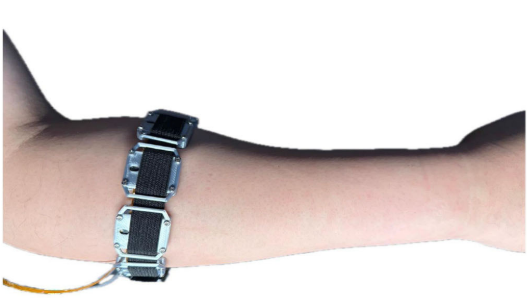
\includegraphics[width=0.5\linewidth]{EMG.png}
    \caption{An EMG armband capable of classifying 6 gestures with 97.8\% accuracy \cite{Aghchehli2025MediumRecognition}}
    \label{fig:emg}
\end{figure}

\subsection{Magnetomyography}
Magnetomyography measures the magnetic fields generated by muscle contractions. It has multiple advantages over EMG - it is less affected by changes in skin conductivity and doesn't rely on sensor coupling with the skin. Yun et al. showed magnetomyography can classify 9 gestures with 95\% accuracy, and can generalise well across participants \cite{IncRichyYun2024GeneralizableMagnetomyography}. However, magnetomyography requires extremely expensive sensing equipment, as well as a magnetically shielded room, making it unsuitable for low cost, portable gesture recognition.

\subsection{Mechanomyography (MMG)}
Mechanomyography is a technique that measures the mechanical oscillations caused by muscle contractions, typically using accelerometers or microphones. Compared to EMG, MMG is less affected by electrical interference and skin conductivity. MMG has been used to classify 6 hand gestures with 85\% accuracy, and 10 hand gestures with 82\% accuracy, shown in \autoref{fig:mmg}. However, MMG systems are extremely sensitive to environmental noise and body movement, limiting their ability to detect subtle gestures and making them impractical for practical everyday use. \cite{Elyasi2025GestureMechanomyography}

\begin{figure}[h]
    \centering
    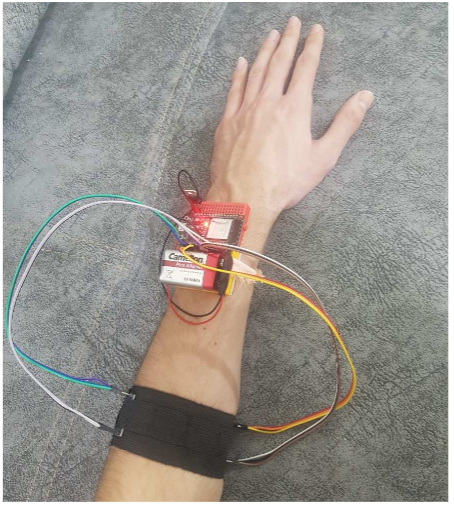
\includegraphics[width=0.5\linewidth]{MMG.png}
    \caption{An MMG wristband capable of classifying 6 hand gestures with 85\% accuracy \cite{Elyasi2025GestureMechanomyography}}
    \label{fig:mmg}
\end{figure}

\subsection{Ultrasound}
Ultrasound imaging can capture muscle and tendon movements in the wrist. EchoFlex \cite{McIntosh2017EchoFlex:Imaging} used ultrasound to classify 10 hand gestures with over 98\% accuracy. However, ultrasound machines are large and have high power consumption. Smaller portable ultrasound scanners are available, but they are expensive. Also, ultrasound devices rely on gel to increase coupling between the transducer and the skin, making them impractical for everyday wearable technology.
\subsection{Optical Tomography and Optomyography (OMG)}
NIR diffuse optical tomography is a 3D imaging technique that uses infrared emitters and receivers to construct 3D distributions of the optical properties of different tissue types. This demonstrates that NIR light can be used to extract useful structural information from tissue.

Optomyography (OMG) is a similar technique that uses infrared emitters and receivers to monitor muscle activity. OMG offers a better signal-to-noise ratio than EMG and MMG, and is less susceptible to factors such as sensor placement and sensor-skin coupling. Previous research has demonstrated that an OMG armband can measure distinct signals for different hand positions, providing further support for using IR light for wrist based gesture recognition. \cite{Muhammed2017AOMG}
\subsection{Infrared Sensing}
Infrared sensing systems measure the interaction of infrared light with biological tissue. Optomyography is a technique that uses infrared light to monitor muscle activity. Previous work has shown that infrared sensing and optomyography can be used in wrist worn devices to perform gesture recognition.
\subsubsection{SensIR}
SensIR \cite{McIntosh2017SensIR:Reflection} demonstrated that the interaction of IR light with the wrist can be used to accurately classify hand gestures. It consists of 14 segments, each containing an 860 nm LED and a photodiode, which were used to measure the transmission, reflection, and absorption of IR light as it passed through the wrist. Measurements were taken between all combinations of IR emitters and receivers, and the resulting data was fed into a small neural network which classified the gestures. SensIR classified 12 gestures with an average accuracy of 93\%.
\subsubsection{GestIR}
GestIR \cite{diamand2025} extended SensIR's work by building a modular wristband, enabling LEDs to be more easily interchanged. This allowed for a comparative study of 860 nm, 890 nm, and 950 nm LEDs, identifying 860nm as the most effective wavelength. GestIR also evaluated a range of machine learning models, identifying a large neural network as the most effective.

GestIR and SensIR both used bulky, hand soldered through hole components. Repeated flexing meant solder joints were prone to breaking, and physical space constraints meant a second PCB was required to house electrical components. Also, suitable through hole LEDs are difficult to source. This meant there were limited LEDs available to test, and complex manufacturing processes such as dedoming of LEDs were required.

FlexIR addresses these issues by using a flexible PCB wristband. This improves on the practicality and ergonomics by reducing the form factor of the device, and allows for the comparison of a wider range of surface mount components. It also simplifies the manufacturing process, since third party PCBA services can be used.

\subsubsection{Realtime gesture decoding}
Recent concurrent work by Khalikov et al. used a flexible PCB wristband design to decode hand gestures in real time \cite{Khalikov2026WearableControl}. In the study, users wore a wristband that measured the interaction of IR light with the wrist, similar to SensIR and GestIR. Users completed a calibration process, where they performed a variety of hand gestures. A small machine learning model was then trained on the data. After calibration, users used the device to play a cursor-pointing game where they used hand gestures to acquire targets with a screen cursor. While the study also used a flexible PCB wristband, the hardware design and study goals differ from this project:
\begin{itemize}
    \item A layer of transparent silicon was used to cover the LEDs and photodiodes. While potentially beneficial for ergonomics, the effect of introducing extra materials on the path of the light is unclear. This removes the possibility for accurate comparison of the optical properties of components, e.g. LED viewing angle. In this project, the sensing hardware makes direct contact with the skin.
    \item FlexIR achieves a much higher component density, containing 16 segments capable of emitting and receiving IR light, allowing for more data collection.
\end{itemize}

Nonetheless, the study demonstrated the viability of flexible PCBs for infrared based gesture recognition, further justifying the design choices for this project. Also, it shows that infrared sensing wristbands have the potential to allow real world, real time gesture based interaction and control over computers.
% Khalikov et al. used optomyography to decode hand gestures in real time \cite{Khalikov2026WearableControl}. In the study, users wore a wristband that measured the interaction of IR light with the wrist, similar to SensIR. Users completed a callibration process, where they performed a variety of hand gestures. A small machine learning model was then trained on the data. After callibration, users used the device to play a cursor-pointing game where they used hand gestures to acquire targets with a screen cursor. This shows that infrared sensing wristbands have the potential to allow real world, real time gesture based interaction and control over computers.



% The Khalikov et al. study used a flexible printed circuit board (FPCB) design. This makes the wristband more compact, improving the ergonomics and practicality.

% In this project, we also designed and manufactured a flexible PCB wristband. However, the FlexIR wristband has a higher component density than the wristband used in the Khalikov study, containing more infrared emitters and sensors, allowing for more data collection. The form factor of the FlexIR wristband is also smaller, further improving ergonomics and practicality. In this project, the sensing hardware (LEDs and photodiodes) makes physical contact with the skin, whereas the Khalikov study used silicon covers over the electronics. This enables FlexIR to more effectively isolate the optical properties of components, e.g. LED viewing angle, for investigation.

\section{Hardware}
\label{section:hardware}
This section is an overview of the electronic components required to manufacture an infrared sensing system.

\subsection{PCBs}
A Printed Circuit Board (PCB) is a thin board made of alternating layers of conductive material (e.g. copper) and insulating substrate (e.g. FR-4). The conductive copper layers are laid out in tracks and are used to connect electronic components together \cite{Grout2008DigitalCPLDs}.

A Flexible Printed Circuit Board (FPCB) is a PCB that uses a flexible material (e.g. polyimide) as a substrate. FPCBs are useful for wearable devices since the electronics can bend and conform easily to the body. Stiffeners are rigid materials attached to portions of an FPCB to provide reinforcement to specific parts of the circuit. Stiffeners are commonly used underneath components to prevent bending, avoiding broken solder joints \cite{2009FlexibleElectronics}.

\subsection{Through Hole Technology (THT) and Surface Mount Technology (SMT)}
Electrical components can be attached to PCBs using either Through Hole Technology (THT) or Surface Mount Technology. THT is when component leads are inserted through holes drilled in PCBs and soldered to pads on the opposite side (\autoref{fig:tht}). SMT is a method where components are mounted directly to the surface of a PCB (\autoref{fig:smt}). Components mounted using SMT are called Surface Mount Devices (SMDs) \cite{Horowitz2015TheEdition}.


\begin{figure}[h]
     \centering
     \begin{subfigure}[b]{0.35\textwidth}
         \centering
         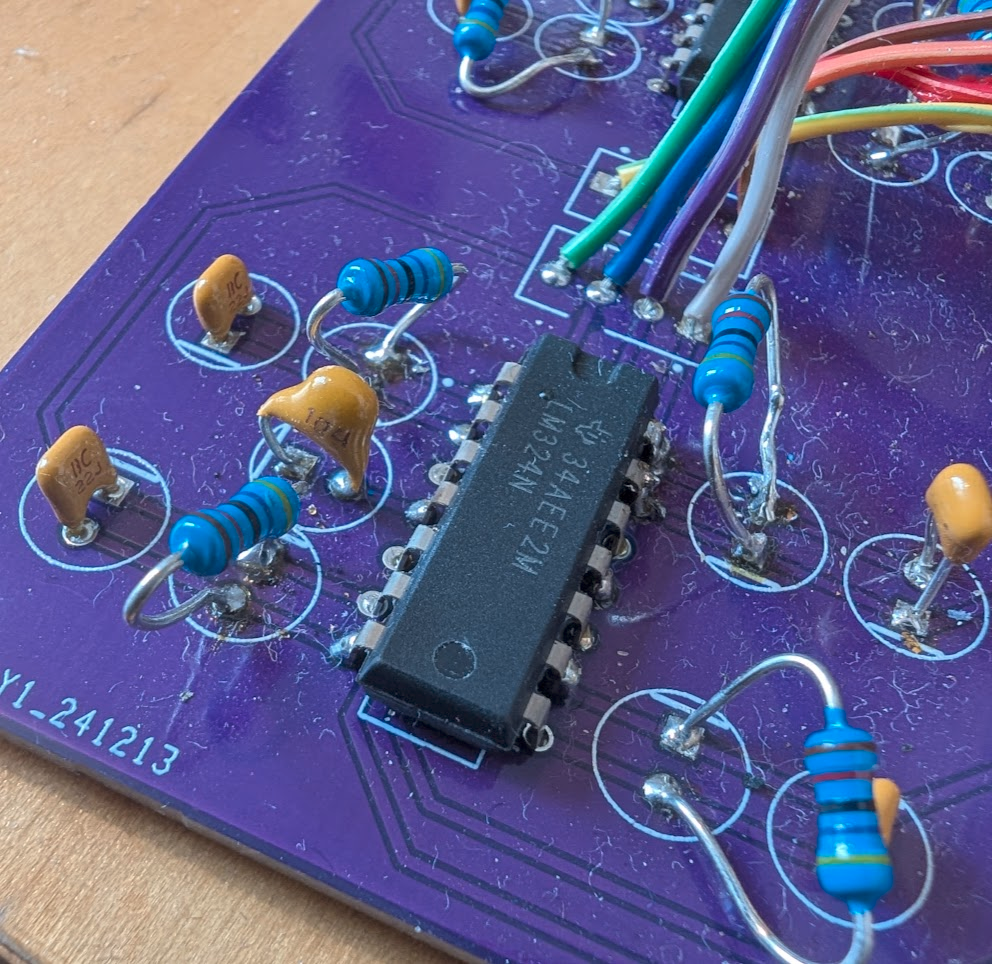
\includegraphics[width=\textwidth]{THT.png}
         \caption{Through Hole Technology (THT)}
        \label{fig:tht}
     \end{subfigure}
      \begin{subfigure}[b]{0.35\textwidth}
         \centering
         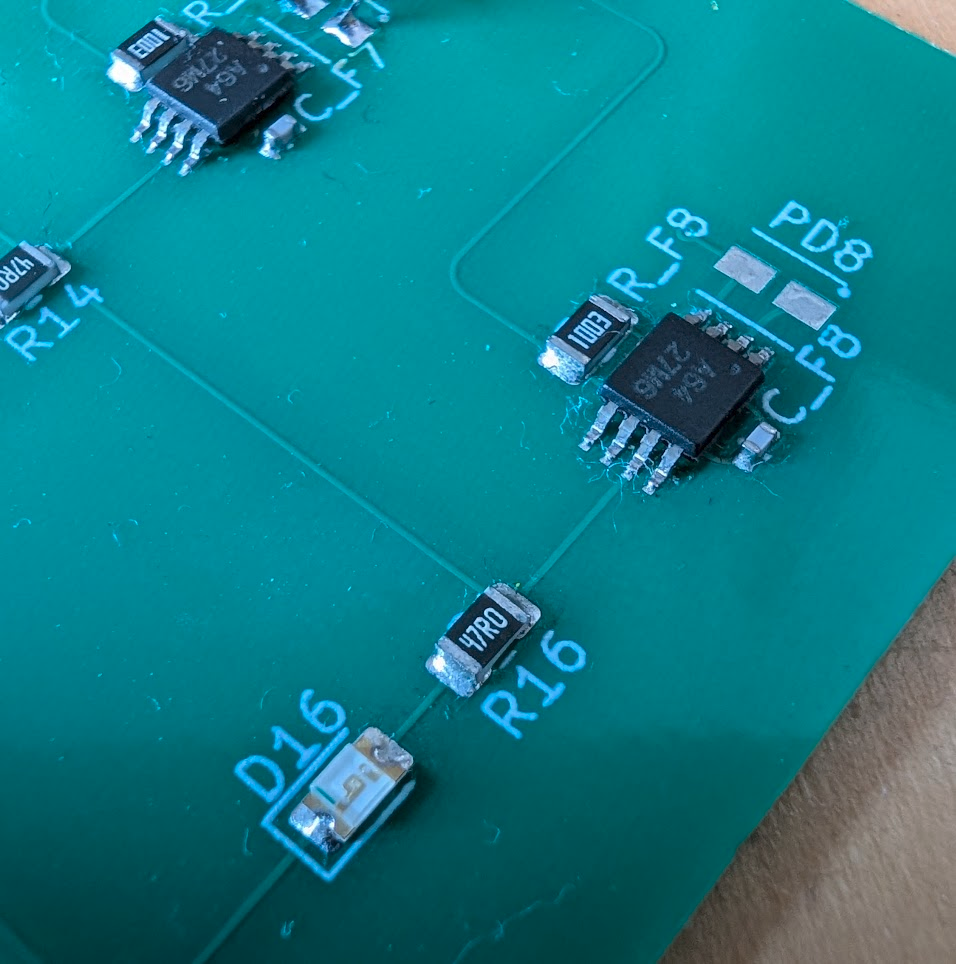
\includegraphics[width=\textwidth]{SMT.png}
        \caption{Surface Mount Technology (SMT)}
        \label{fig:smt}
     \end{subfigure}
    \caption{Methods of mounting components to PCBs}
    \label{fig:tht_smt}
\end{figure}

\subsection{LEDs}
A diode is an electrical component that only allows the flow of current in one direction \cite{Horowitz2015TheEdition}. An LED is a diode that converts electrical energy into light. The angle of half intensity, or viewing angle, of an LED is the angle at which the intensity of the light is half the maximum intensity of the LED. 

Radiant power is the total amount of optical power emitted from an LED. Radiant intensity is the radiant power per solid angle. LEDs with the same radiant power but smaller viewing angles have higher radiant intensities \cite{Schubert2006Light-EmittingDiodes}.

\subsection{Photodiodes}
Photodiodes are semiconductors that convert light into electrical energy. When light hits a photodiode, it generates a small current \cite{Horowitz2015TheEdition}.
\subsection{Transistors/Darlington Pairs}
Transistors are components used to control the flow of electricity. They have three terminals: the collector, base, and emitter. A small current applied to the base allows a large current to flow from the collector to the emitter. The current gain, \(h_{fe}\), of a transistor is the ratio of collector current to base current.

For applications that require high collector currents and low base currents, a Darlington pair can be used to increase the current gain. A Darlington pair is a configuration of two transistors that acts as one composite transistor with a larger current gain. The current gain of a Darlington pair is the product of the gain of the two transistors \cite{Horowitz2015TheEdition}.
\subsection{Shift Registers}
A Serial-In-Parallel-Out (SIPO) shift register is a component that can store and shift bits. It contains a cascade of flip-flops (small circuits that can store 1 bit of data). When the clock pin on the shift register is pulsed, the data in the shift register is shifted one position to the right and the new data is saved in the first flip-flop. The output of each flip-flop is connected to an output pin. SIPO shift registers can be used to reduce the number of output pins required on a microcontroller by using serial data to control circuits rather than directly connecting other components to the microcontroller pins \cite{Holdsworth2007DigitalDesign}.

\subsection{Transimpedance Amplifiers}
Transimpedance amplifiers are current to voltage converters that can be used to amplify photodiode signals. They convert the small current produced by the photodiodes into larger voltages that can be measured by a microcontroller. A transimpedance amplifier consists of an op-amp and a feedback resistor. The    output voltage, \(V_{out}\), is defined as:

\[V_{out} = -I_{in} * R_f\]

where \(I_{in}\) is the input current and \(R_f\) is the value of the feedback resistor \cite{TexasInstrumentsWhat1}.

\section{Microcontrollers}
Microcontrollers are small computers on a single integrated circuit. Code can be run on microcontrollers to control other electrical components through output pins, and to read signals through input pins. Most microcontrollers have analogue-to-digital converters (ADCs), which convert analogue signals at the input pins to binary numbers that the processor can manipulate. The conversion rate of an ADC is how fast it can convert an analogue value to a digital value. The resolution of an ADC is the smallest change in an analogue signal that would result in a change in the digital output.

\section{Machine Learning}
Machine learning models are programs trained on datasets to identify patterns and make predictions. In this project, we used machine learning models to classify hand gestures based on infrared sensor data. This section is an overview of the models used.

\subsection{Classification Task}
A classification task is a machine learning task that assigns predefined labels or categories to input data. Classification is a supervised learning approach, meaning models are trained on labelled training data. There are two main evaluation metrics:
\begin{itemize}
    \item \textbf{Accuracy} - the accuracy is the proportion of unseen test data the model can correctly label
    \item \textbf{Confusion Matrices} - a confusion matrix is a table showing which label the model assigned to each piece of data. Each row of the matrix represents the true label and each column represents the predicted label, or vice versa. Confusion matrices can be used to identify how effective the model is at classifying each class.
\end{itemize}

\subsection{Decision Trees}
Decision Trees are models that classify data points by following a tree structure from root to leaf. At each node, a feature is tested against a decision boundary to decide which edge to follow. A class label is assigned when a leaf is reached.
\subsection{Random Forests}
Random forests are ensemble methods that consist of multiple decision trees, each of which are trained on random subsets of the dataset. The final prediction is an aggregate of all the decision tree predictions. 
\subsection{Neural Networks}
Neural networks are models made up of layers of interconnected neurons. They learn complex relationships between features using backpropagation and gradient descent.
\subsubsection{Multi Layer Perceptrons (MLP)s}
An MLP is the most common type of neural network. It consists of:
\begin{itemize}
    \item An input layer, where each neuron corresponds to a feature of the input data
    \item One or more hidden layers, which contain interconnected neurons that learn relationships between features
    \item An output layer, which produces the models predictions. In a classification task, there is one neuron per class label.
\end{itemize}
\subsubsection{Convolutional Neural Networks (CNN)s}
A CNN is a type of neural network that is more effective at processing grid-like data, e.g. image data. In a CNN, a filter (or kernel) slides across the input data, performing an operation with the part of the data it's over at each step. The resulting number is stored as a feature.

CNNs have convolutional layers, which use filters to extract useful structural features from the input data, for example to perform edge detection in images.

They also have pooling layers, which replace outputs from the previous layer with a summary statistic. For example, the max pooling function outputs the maximum value in a rectangular neighbourhood. Pooling is used to reduce the size of the feature maps and improve invariance to small translations of input data.

\subsubsection{Training Neural Networks}
Training a Neural Network involves three steps:
\begin{itemize}
    \item Forward propagation - this is when the input is passed through the network to produce an output
    \item A loss function evaluates how good the models prediction was
    \item Backpropagation is used to move back through the network and calculate the error of each neuron
    \item An optimisation algorithm is used to update the network weights
\end{itemize}

\subsubsection{Overfitting and Regularization}
Regularization helps prevent neural networks overfitting to training data. Some common techniques include:
\begin{itemize}
    \item \textbf{L1 and L2 regularization} both alter the loss function to penalize large weights. L1 regularization adds the sum of the neuron weights multiplied by a constant, and L2 regularization adds the sum of the squared weights multiplied by a constant.
    \item \textbf{Early stopping} - if the validation performance doesn't increase after a certain amount of time, training is halted.
    \item \textbf{Dropout} is a technique that randomly sets a small amount of neurons to zero each training step, to prevent over reliance on specific neurons.

\end{itemize}

\subsubsection{Monte Carlo Dropout}
Monte Carlo dropout is an ensemble approach that can be used to improve performance of neural networks. Random dropout is enabled during model inference, meaning the model output is non deterministic for the same input. By aggregating multiple predictions, the model accuracy can be improved.

\section{Biology}
Three main phenomena occur when IR light interacts with biological tissue: \textbf{reflection, absorption }and\textbf{ scattering} \cite{diamand2025}.

\begin{itemize}
    \item \textbf{Reflection} - light reflects when it hits the boundary between two materials. 
    \item \textbf{Absorption} - materials have an absorption coefficient, which measures how strongly it absorbs light per unit distance.
    \item \textbf{Scattering} - light bounces as it travels through tissue, changing direction.
\end{itemize}

The \textbf{first optical window}, also known as the NIR 1 window, is a range of wavelengths commonly used in medical imaging (650 - 950 nm). The absorption coefficients of tissue materials are low for these wavelengths, making them effective at penetrating flesh.

% -----------------------------------------------------------------------------

\chapter{Designing and Manufacturing the Wristband}
\label{chap:execution}
The FlexIR wristband, shown in \autoref{fig:FlexIR_wrist}, performs gesture recognition by measuring the transmission and reflection of near IR light through the wrist.

\begin{figure}[htp]
    \centering
    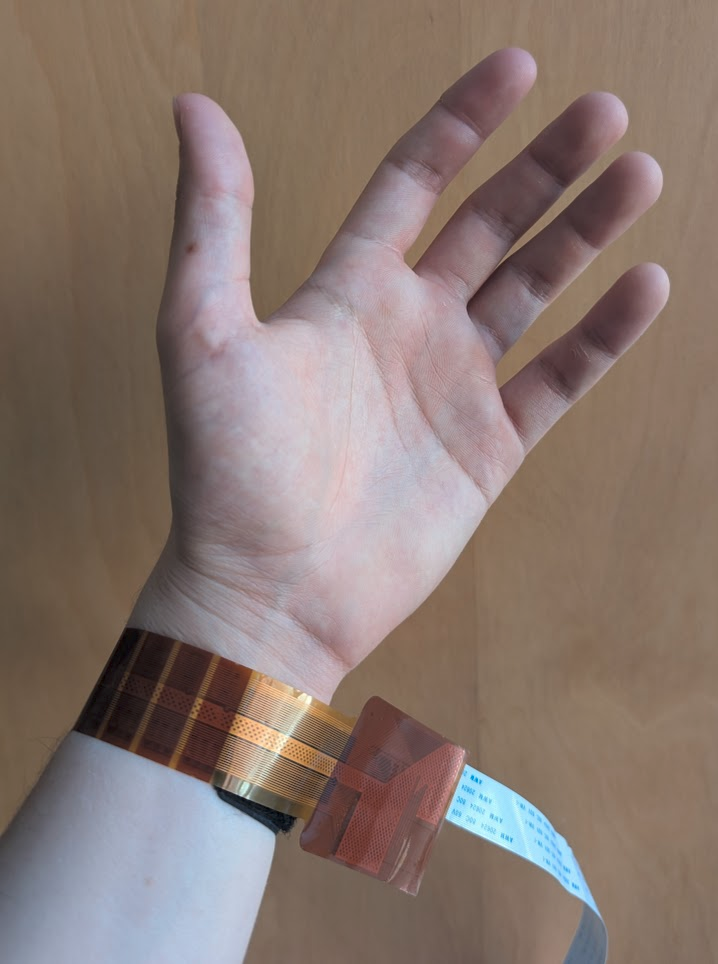
\includegraphics[width=0.5\linewidth]{FlexIR_wrist.png}
    \caption{FlexIR wristband}
    \label{fig:FlexIR_wrist}
\end{figure}

FlexIR improves on the designs of SensIR \cite{McIntosh2017SensIR:Reflection} and GestIR \cite{diamand2025} by using a flexible PCB as the main body of the wristband, with small surface mount components. This has multiple benefits over previous designs:

\begin{itemize}
    \item SMD components are smaller than through hole components, meaning  
    \begin{itemize}
        \item More of the circuit fits onto the main wristband. This removes the need for a second PCB.
        \item Placing transimpedance amplifiers physically closer to the photodiodes reduces the input capacitance of the amplifiers, resulting in higher quality measurements with less noise.\cite{Horowitz2015TheEdition}
        \item More LEDs fit on the wristband, increasing the amount of IR light produced.
    \end{itemize}
    \item The addition of shift registers on the wristband for LED activation reduces the number of cables needed between the wristband and microcontroller

    \item Third party PCB manufacturers can be used for fabrication and assembly, meaning
    \begin{itemize}
        \item Multiple wristbands can be manufactured quickly, to repeatable high standards
        \item PCBs are more robust and reliable than previous handmade designs.
    \end{itemize}
    \item There is a wider range of SMD components available, enabling easier comparison between LEDs
\end{itemize}

Compared to the FPCB wristband used in the Khalikov et al. study, the FlexIR wristband also has design differences that better qualify it for this study:
\begin{itemize}
    \item FlexIR has a higher density of components, containing 16 segments of LEDs and photodiodes. FlexIR produces 256 measurements for each reading.
    \item The sensing hardware in FlexIR makes direct contact with the skin, allowing for direct comparison of optical properties of components, e.g. LED viewing angle.
\end{itemize}

\section{Operating Principle}
\label{sec:operating_principle}
\begin{figure}[h]
     \centering
     \begin{subfigure}[b]{0.4\textwidth}
         \centering
         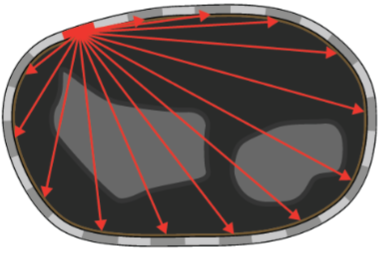
\includegraphics[width=\textwidth]{SensIR.png}
         \caption{One LED is activated and all photodiode values are measured \cite{McIntosh2017SensIR:Reflection}}
        \label{fig:SensIR}
     \end{subfigure}
      \begin{subfigure}[b]{0.4\textwidth}
         \centering
         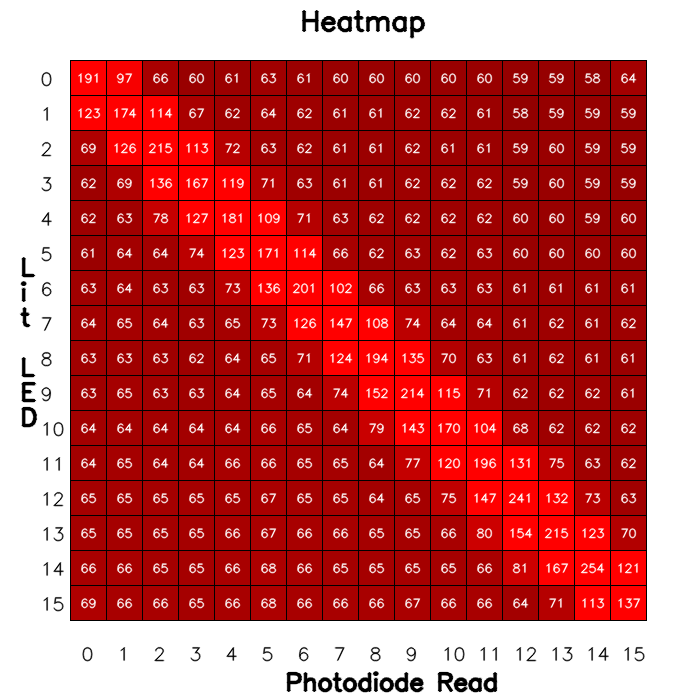
\includegraphics[width=\textwidth]{figures/heatmap_all.png}
        \caption{A 16x16 reading from the wristband}
        \label{fig:heatmap_all}
     \end{subfigure}
    \caption{FlexIR operating principle}
    \label{fig:operation}
\end{figure}
The FlexIR wristband is made up of 16 segments, each containing 3 LEDs and a photodiode. The wristband is connected to a Teensy 4.1 microcontroller via a flat flexible cable (FFC). The microcontroller sequentially activates each group of 3 LEDs and records the values measured by all the photodiodes (\autoref{fig:SensIR}). This produces a 16x16 reading (\autoref{fig:heatmap_all}) containing data from every combination of LEDs and photodiodes, which can be used to classify hand gestures.

\section{Wristband Design}

\subsection{Overview}
\begin{figure}[htp]
    \centering
    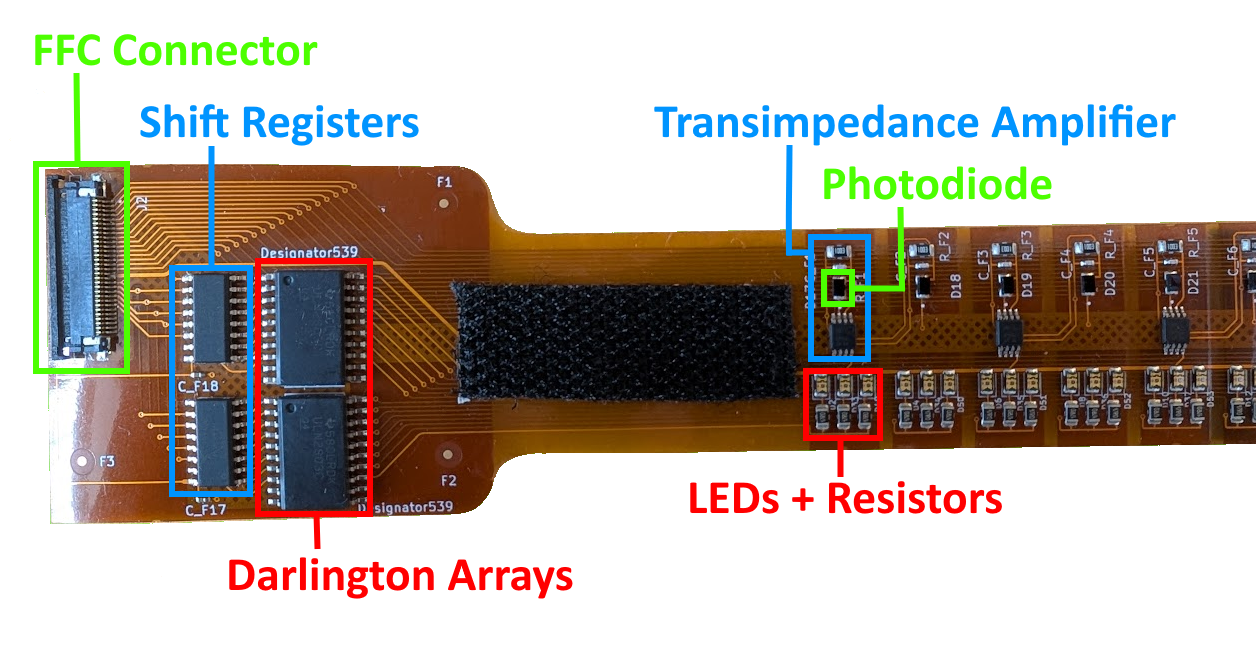
\includegraphics[width=\linewidth]{FlexIR_new.png}
    \caption{Design of the FlexIR wristband}
    \label{fig:FlexIR}
\end{figure}

The wristband is based on a flexible PCB, shown in \autoref{fig:FlexIR}. There are two main sections: the head and the body. The head of the wristband contains two 74HC595D shift registers and two ULN2803C Darlington arrays which are used to drive the LEDs. It also contains an FFC connector, which is used to connect the device to a microcontroller. The main body of the wristband contains 16 stiffened segments. Each segment contains three LEDs, a photodiode and a transimpedance amplifier. Between the head and the body, there is a large empty section of the PCB which is used for fastening.

\subsection{Stiffeners}
PCB stiffeners are extra layers of material applied to flexible PCBs to provide rigidity in specific locations. 

Stiffeners are used in FlexIR on the wristband head, as well as each of the 16 segments. This stops the wristband flexing underneath the large SMD components, which helps prevent broken solder joints, shown in \autoref{fig:stiffener}.

\begin{figure}[htp]
    \centering
    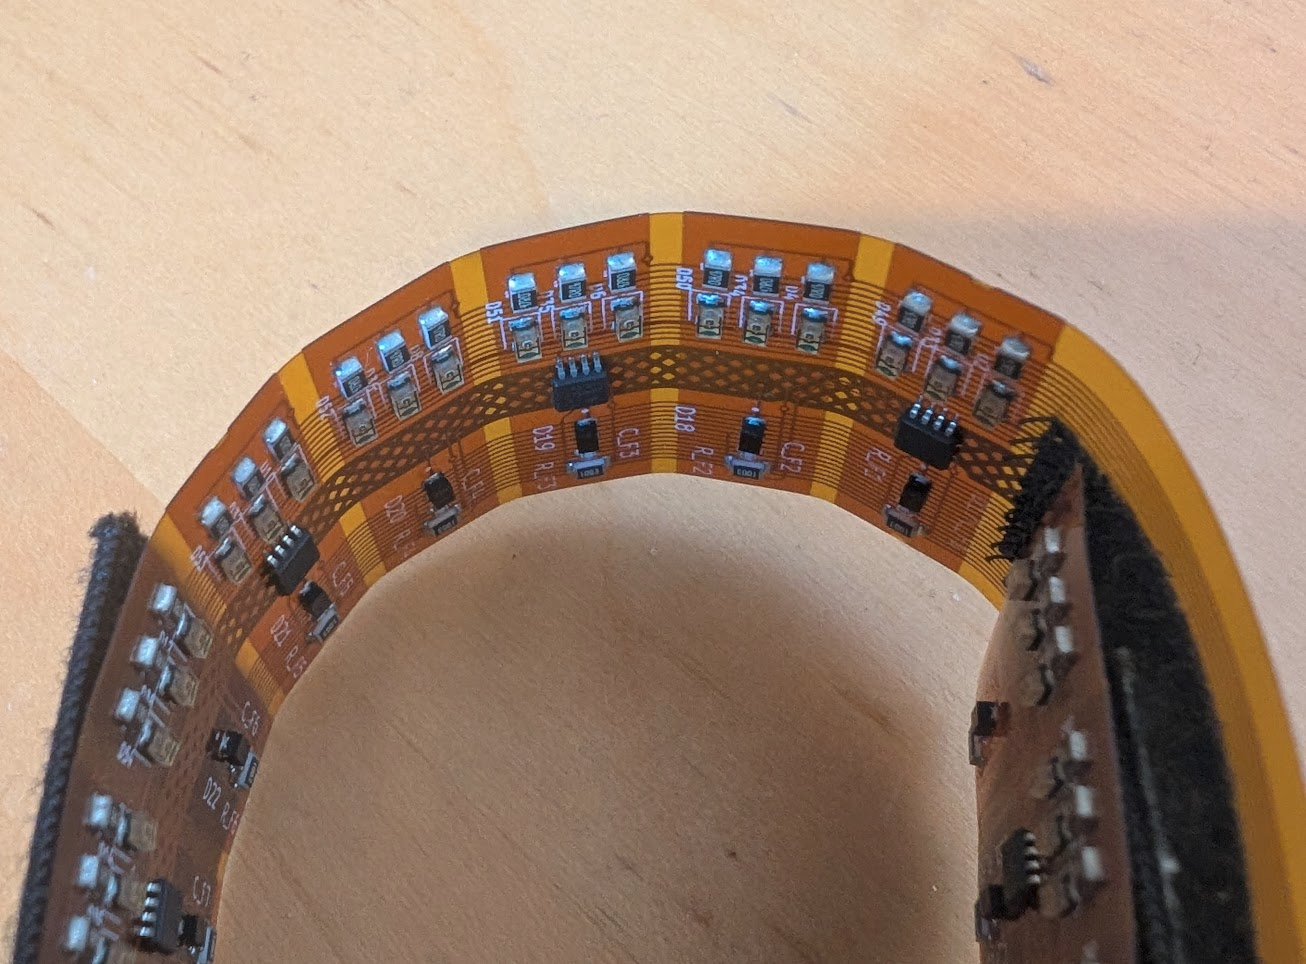
\includegraphics[width=0.5\linewidth]{stiffener.png}
    \caption{The stiffener on the back of the FlexIR wristband prevents the PCB bending underneath the components.}
    \label{fig:stiffener}
\end{figure}

\subsection{Fastening}
Flexible PCBs cannot be stretched, so a mechanism is needed to fix the wristband in place once it is placed around a users wrist. The wrist circumference also varies significantly as users perform different hand gestures.

An early prototype used a pin buckle, similar to a watch strap, to fasten the wristband. However, we found that due to the taper of the wrist, it was useful to fasten the ends of the wristband at a range of angles. Another prototype, shown in \autoref{fig:prototype}, consisted of a Velcro pad glued to a large empty section of the PCB and another pad glued to the stiffeners on the back. This allowed the wristband to fasten around any wrist thickness at any angle, but didn't accommodate for changes in wrist circumference throughout usage.

\begin{figure}[htp]
    \centering
    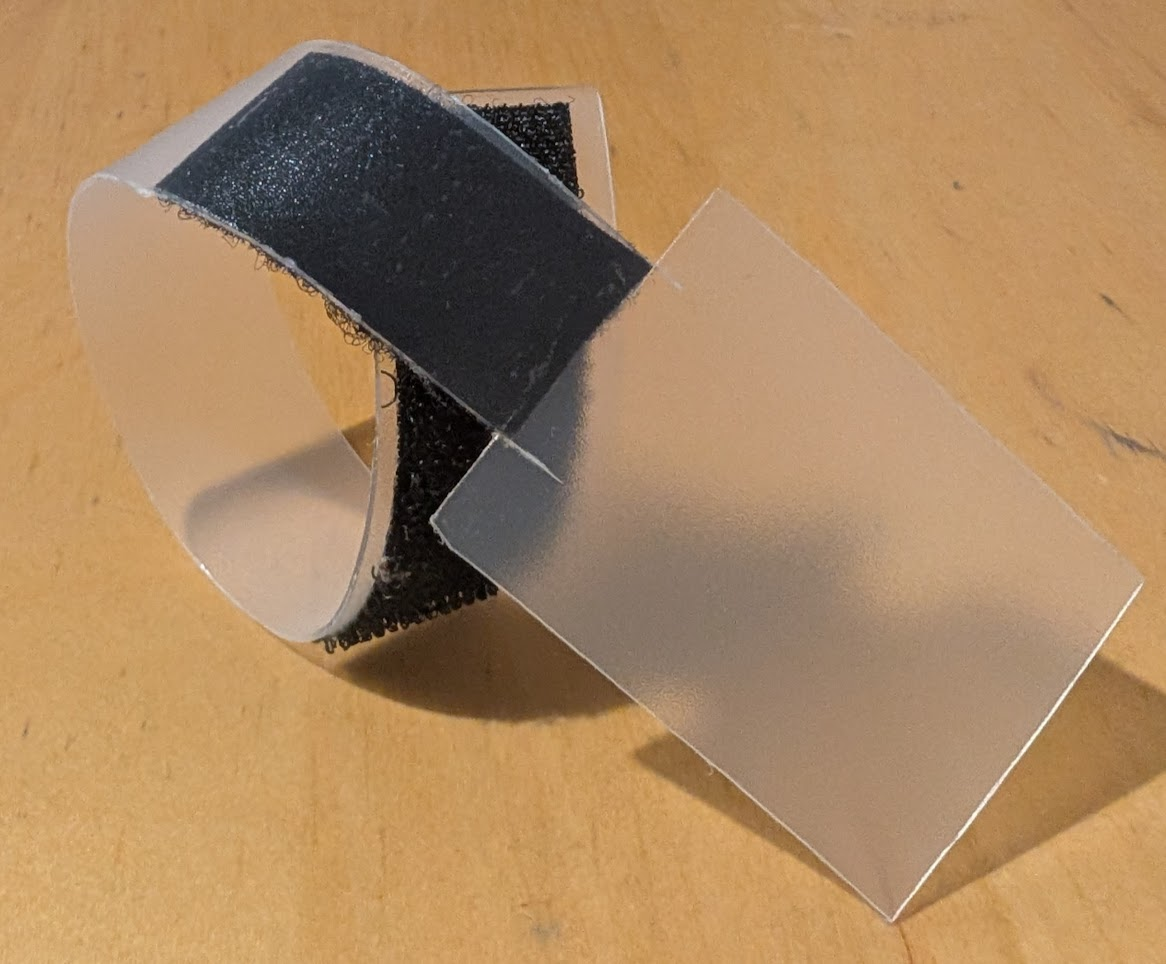
\includegraphics[width=0.33\linewidth]{FlexIR-prototype.jpg}
    \caption{Initial prototype - the wristband can be fastened at an angle, accommodating for the natural taper of the wrist}
    \label{fig:prototype}
\end{figure}

The final design uses one Velcro pad glued to a large empty section of the PCB, and another Velcro pad attached to an elastic strap, which is glued to the stiffeners on the back of the PCB (\autoref{fig:final_strap}). The wristband can be fastened tightly around the wrist, and has the ability to expand and constrict as the user performs gestures.

\begin{figure}[htp]
    \centering
    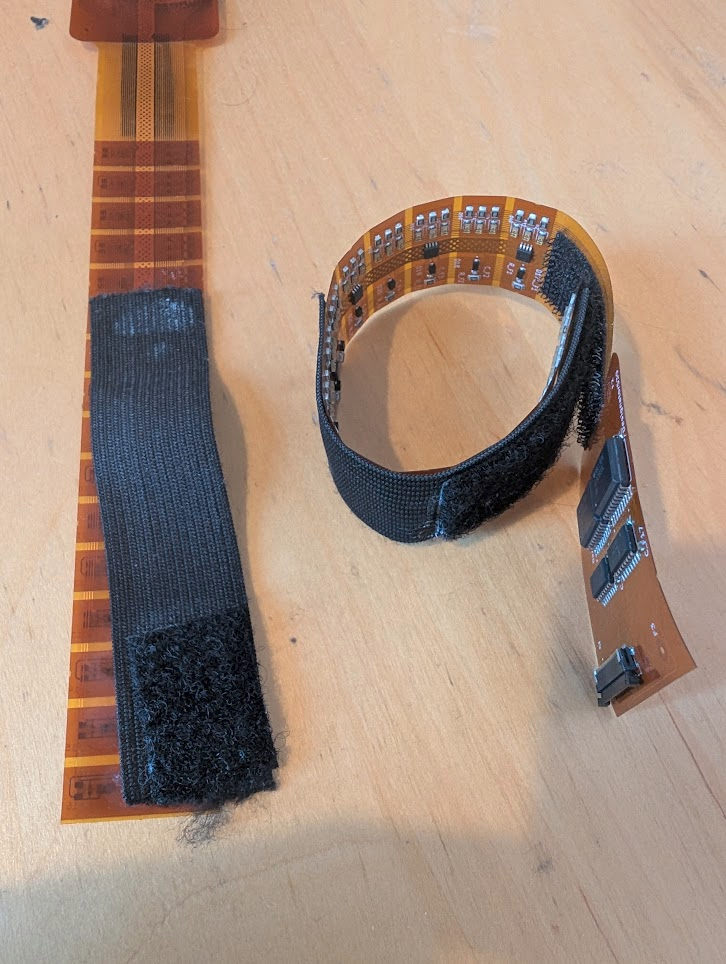
\includegraphics[width=0.33\linewidth]{final_strap.png}
    \caption{Final fastening mechanism - a Velcro pad is glued to an elastic strip which is glued to the back stiffeners}
    \label{fig:final_strap}
\end{figure}

\section{Circuit}
The electronic components on the FlexIR wristband make up two circuits: the LED circuit, used to activate the IR LEDs, and the sensing circuit, used to measure photodiode readings. This section explains the design of the circuits and the components used. See \autoref{section:hardware} for the necessary background.

\subsection{LED Circuit}
Each of the 16 wristband segments contain 3 IR emitting LEDs, which are controlled by shift registers and Darlington arrays located on the head of the wristband.

\subsubsection{Shift Registers}
Each LED and photodiode must be individually controllable. To reduce the number of wires required between the wristband and microcontroller, we used 74HC595D shift registers for LED activation. Daisy chaining two 74HC595D chips allows for the control of 16 LEDs using 5 output pins of the microcontroller.

\subsubsection{Darlington Arrays}
The microcontroller pins can't provide enough power to activate the LEDs, so we used ULN2803C Darlington arrays. Power is supplied to the anode of each LED through a thick shared power trace running through the center of the PCB, and the cathode of each LED is connected to an output of a ULN2803C. When an input on one of the ULN2803C chips is activated, the corresponding output is connected to ground, and current flows through the LED. The inputs of the ULN2803Cs are activated by the outputs of two 74HC595D shift registers.

\subsubsection{LEDs}
When the microcontroller stores a bit in a shift register, the corresponding output is activated. This activates an input on one of the Darlington arrays, which connects the corresponding output to ground, allowing current to flow through one of the LEDs. Each LED is wired in series with a 47R resistor, which limits the current.

\subsection{Sensing Circuit}
Each of the 16 wristband segments contains a photodiode, which senses the level of IR light, and a transimpedance amplifier, which converts the small output current of the photodiode into a measurable voltage.
\subsubsection{Photodiodes}
The photodiode is connected to power through the large central power trace, and to ground through the hatched ground plane. When IR light hits the photodiodes, a small current is generated.
\subsubsection{Transimpedance Amplifiers}
The transimpedance amplifiers converts the small currents produced by the photodiodes into larger voltages that can be measured by the microcontroller. The transimpedance amplifiers use TLV9062 op-amps configured with a $100 k\Omega$ feedback resistor and a 1 pF capacitor. The output of the transimpedance amplifiers are connected to the analogue input pins of the microcontroller.

\subsection{Microcontroller}
The wristband connects to a Teensy 4.1 microcontroller via an FFC cable, which is plugged into a connector on the head of the wristband. The microcontroller activates the LEDs and reads from the photodiodes as described in \autoref{sec:operating_principle}.

\begin{listing}[ht]
\begin{minted}{c}
void capture() {
    const int NUM_SAMPLES = 5;
    for (int activeLed = 0; activeLed < PIN_COUNT; activeLed++) {
        enableLed(activeLed);
        delayMicroseconds(10);
        for (int readLed = 0; readLed < PIN_COUNT; readLed++) {
            int sum = 0;
            for (int i = 0; i < NUM_SAMPLES; i++) {
                sum += analogRead(PHOTODIODE_PINS[readLed]);
                delayMicroseconds(50);
            }
            captureMatrix[activeLed][readLed] = sum / NUM_SAMPLES;
        }
        disableLed(activeLed);
    }
    printMatrixSerial();
}
\end{minted}
\caption{Microcontroller code to flash LEDs and read photodiode values \cite{diamand2025}}
\label{listing:capture_loop}
\end{listing}

\autoref{listing:capture_loop} shows code which runs on the Teensy, adapted from code provided by GestIR \cite{diamand2025}. The code sequentially activates the LEDs. For each active LED, it records an average of five readings for each photodiode. The Teensy's internal ADCs, with 12 bit resolutions, were used to read the analogue photodiode values.

To control the LEDs, there is a global \mintinline{c}{uint16_t LEDSequence} variable which keeps track of the bits stored in the shift registers. To enable or disable an LED, the corresponding bit of the \mintinline{c}{LEDSequence} variable is set to 1 or 0 and the data is written to the shift register using the built-in Arduino function \mintinline{c}{shiftOut} (\autoref{listing:led_control}).

\begin{listing}[ht]
\begin{minted}{c}
void enableLed(int index) {
    LEDSequence = LEDSequence | ((uint16_t)1 << index);
    byte lowByte = LEDSequence & 0xFF;
    byte highByte = (LEDSequence >> 8) & 0xFF;

    digitalWrite(latchPin, LOW);
    shiftOut(dataPin, clockPin, LSBFIRST, highByte);
    shiftOut(dataPin, clockPin, LSBFIRST, lowByte);
    digitalWrite(latchPin, HIGH);
}

void disableLed(int index) {
    LEDSequence = LEDSequence & ~((uint16_t)1 << index);
    byte lowByte = LEDSequence & 0xFF;
    byte highByte = (LEDSequence >> 8) & 0xFF;

    digitalWrite(latchPin, LOW);
    shiftOut(dataPin, clockPin, LSBFIRST, highByte);
    shiftOut(dataPin, clockPin, LSBFIRST, lowByte);
    digitalWrite(latchPin, HIGH);
}
\end{minted}
\caption{LEDs are activated or deactivated by setting the corresponding bit in the shift register to 1 or 0.}
\label{listing:led_control}
\end{listing}

The microcontroller is connected to a computer, which performs machine learning model training and inference, using a USB cable.

\subsection{Hatched Ground Plane}
Ground planes are large sheets of conductive material used to connect components to ground. Using ground planes reduces the electrical impedance of the ground paths and shields against electromagnetic interference, producing higher quality signals from sensitive circuits like transimpedance amplifiers.

\begin{figure}[htp]
    \centering
    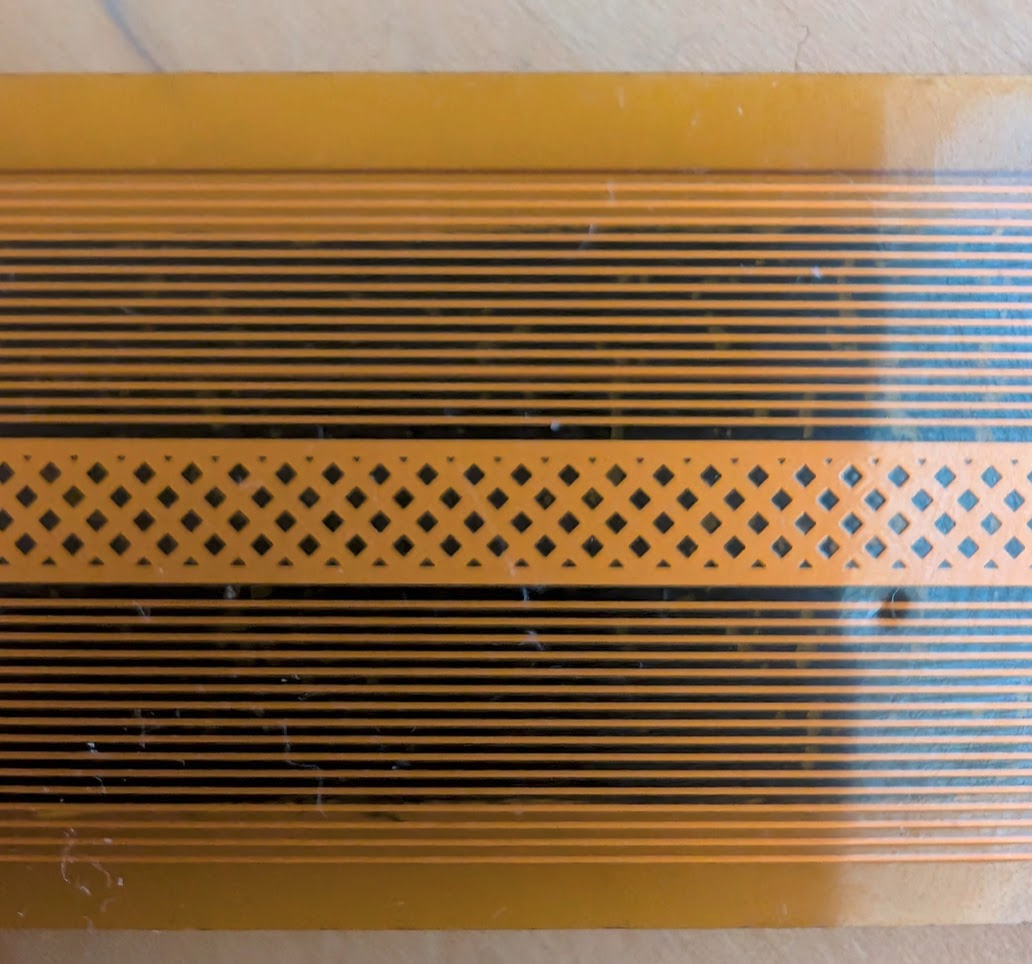
\includegraphics[width=0.3\linewidth]{ground_plane.png}
    \caption{Hatched ground plane on the back of FlexIR}
    \label{fig:ground_plane}
\end{figure}

FlexIR uses a hatched ground plane, shown in \autoref{fig:ground_plane}. This is a ground plane with copper laid out in a mesh pattern rather than a continuous sheet. Hatched ground planes offer the same benefits as regular ground planes while maintaining the flexibility of the PCB.



\section{Wristband Iteration}
\label{section:wristband_iteration}
A major achievement of this project was the design and manufacture of a complex flexible PCB wristband. This was the result of repeated iteration to refine circuit design.

\subsection{Rigid PCB}
\autoref{fig:rigid_pcb} shows an early prototype based on a rigid PCB, consisting of one shift register, one Darlington array, 8 visible light LEDs and 8 IR photodiodes with transimpedance amplifiers. The visible light LEDs allowed easy testing of the LED control and a IR emitting torch was used to test the sensing circuit, before committing to the higher cost and lead time of a flexible PCB.

\begin{figure}[htp]
    \centering
    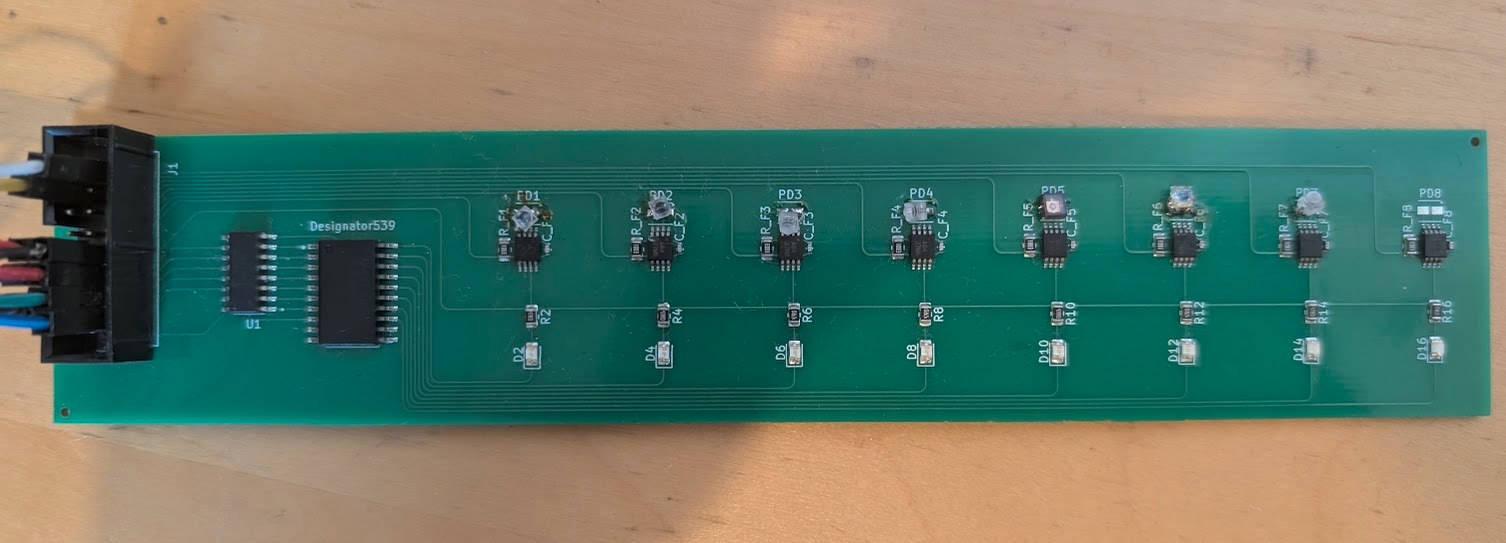
\includegraphics[width=0.6\linewidth]{rigid_pcb.png}
    \caption{Initial rigid PCB prototype}
    \label{fig:rigid_pcb}
\end{figure}

\subsection{Op-amps}
Initial designs of the wristband used one OPA381 \cite{TexasInstruments2004OPA381Amplifier} op-amp for each segment. OPA381s are high precision, low noise op-amps that work well in transimpedance amplifiers with photodiodes. However, the OPA381s were significant contributors to the overall price of the wristband. To reduce the cost, the final design uses the TLV9062 \cite{TexasInstruments2024TLV906xSSystems}, a cheaper, general purpose amplifier with a higher offset voltage and input capacitance. The TLV9062 is also a dual amplifier, with each chip containing two op-amps. In the final wristband design, two adjacent segments share a single TLV9062 chip, shown in \autoref{fig:segments_new}. This halves the number of components needed, further reducing the cost.

\subsection{LEDs}
Initial wristbands were manufactured using one IR17-21C/TR8 LED per segment (\autoref{fig:segments_old}). This allowed us to manufacture multiple iterations of the device, testing other sections of the circuit, without unnecessary spending on higher quality LEDs. Once the circuit design was tested and finalised, final wristbands were manufactured using three brighter, more expensive LEDs per segment (\autoref{fig:segments_new}).

\begin{figure}[h]
     \centering
     \begin{subfigure}[b]{0.35\textwidth}
         \centering
         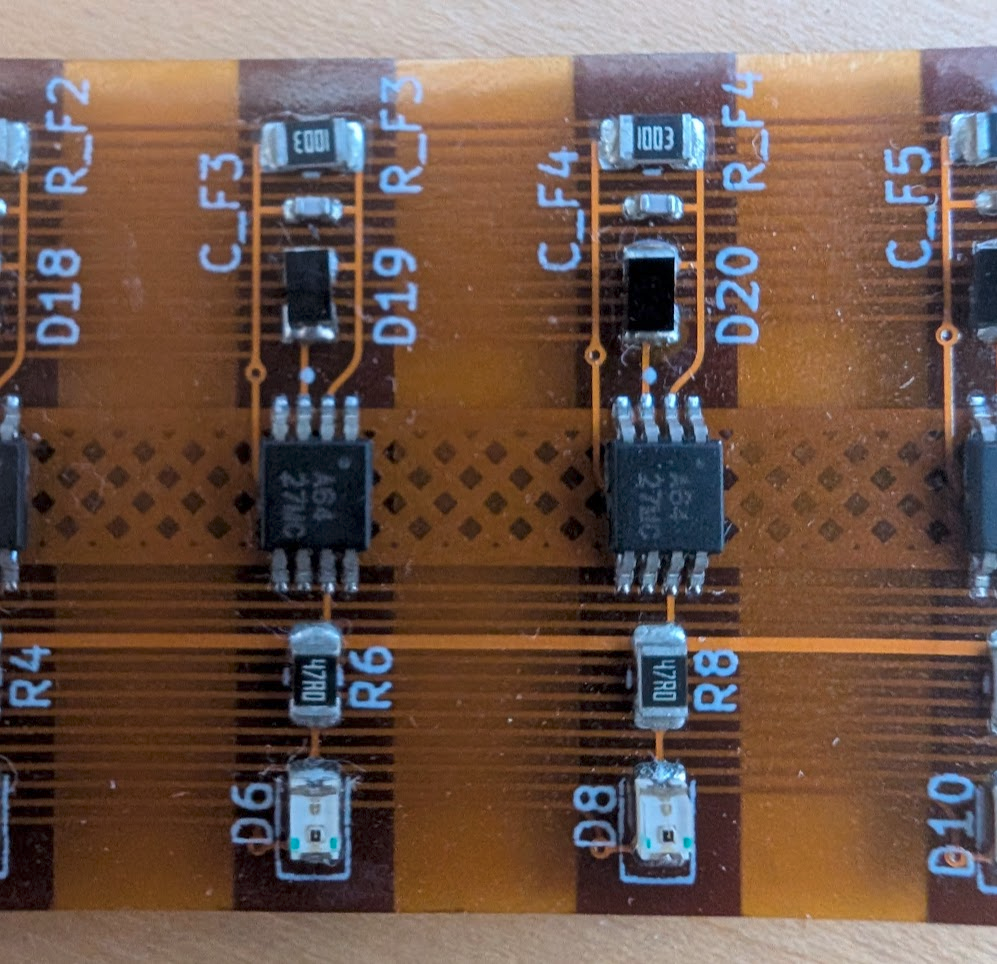
\includegraphics[width=\textwidth]{segments_old.png}
         \caption{Initial design where each segment contains an OPA381 op-amp and one LED}
        \label{fig:segments_old}
     \end{subfigure}
      \begin{subfigure}[b]{0.35\textwidth}
         \centering
         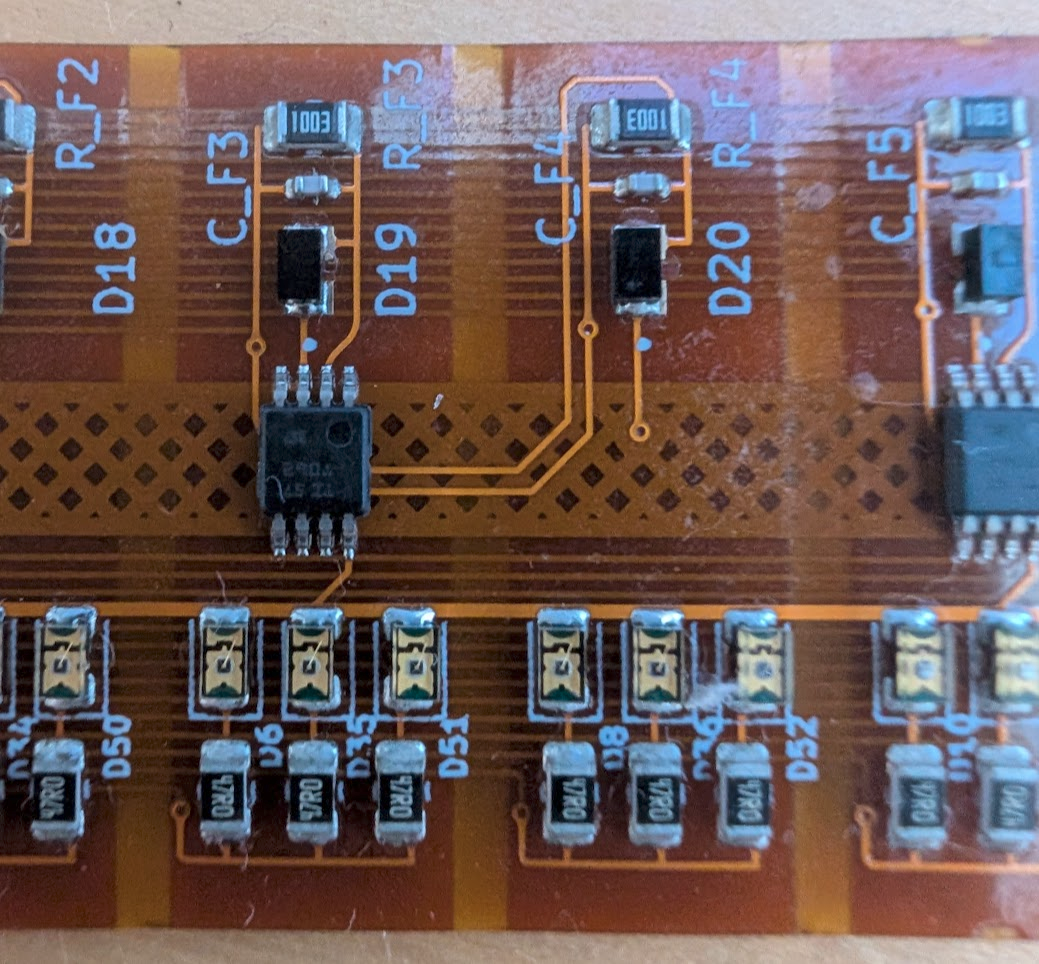
\includegraphics[width=\textwidth]{segments_new.png}
        \caption{Final design where each segment has three LEDs and adjacent segments share a TLV9062 op-amp}
        \label{fig:segments_new}
     \end{subfigure}
    \caption{Adjacent segments in an early design and the final design}
    \label{fig:segments}
\end{figure}


\subsection{Final LED and Photodiode Selection}
We chose to investigate the effect of LED viewing angle on classification accuracy. We selected two LEDs with similar forward voltages and the same total radiant power, but different viewing angles (and radiant intensities).


We hypothesize that:
\begin{itemize}
    \item LEDs with smaller viewing angles will be more effective at penetrating the wrist due to their higher radiant intensity, producing higher quality measurements at photodiodes opposite the active LED.
    \item While LEDs with smaller viewing angles will be less effective at penetrating the wrist, the scattering and reflection of light against tendons close to the surface of the wrist will be more apparent, leading to better results from photodiodes adjacent to the active LED.
\end{itemize}

The selected LEDs had to satisfy the following constraints:

\begin{itemize}
    \item Contrasting viewing angle
    \item Similar radiant power
    \item Small SMD package
\end{itemize}

The LEDs selected were:
\begin{itemize}
    \item The \textbf{VSMB1940X01} \cite{VishaySemiconductors2023VSMB1940X01Nm}, with a $\pm 60^\circ$ viewing angle.
    \item The \textbf{TSML1020} \cite{VishaySemiconductors2017TSML1020Nm}, with a $\pm 12^\circ$ viewing angle.
\end{itemize}

Both LEDs have the same current-voltage graphs and the same radiant power (40 mW at 100 mA). Since they are both powered from the same 3.3 V pin on the Teensy, this means they draw the same amount of current and produce the same amount of light energy. The TSML1020 has a much smaller viewing angle of $\pm 12^\circ$, so the radiant intensity is higher, as shown in \autoref{fig:viewing_angle}.

\begin{figure}[htp]
    \centering
    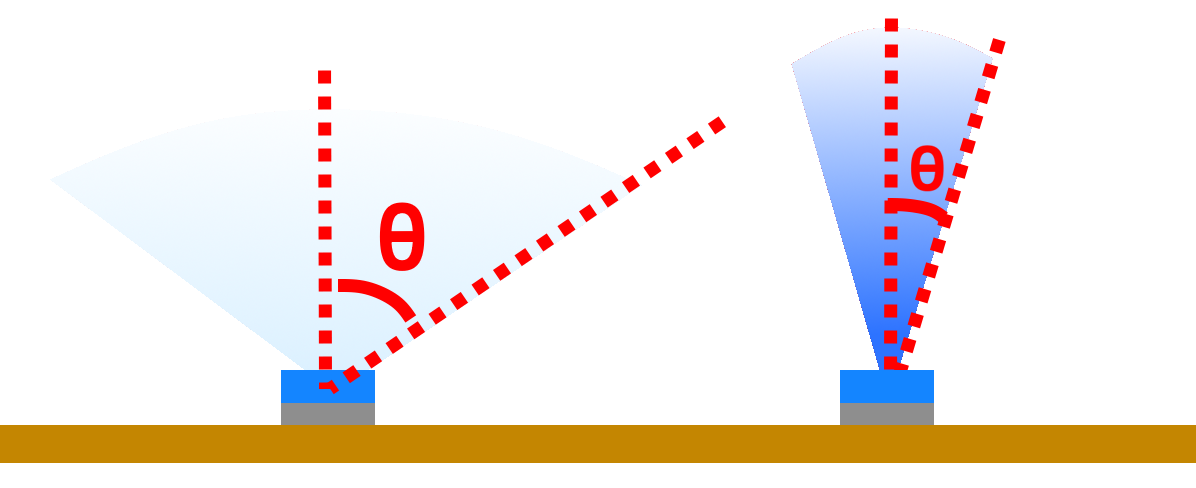
\includegraphics[width=0.6\linewidth]{ViewingAngle.png}
    \caption{LEDs with the same radiant power and different viewing angles have different radiant intensities}
    \label{fig:viewing_angle}
\end{figure}

Both LEDs emit 940 nm wavelength light. Although GestIR identified 860 nm LEDs as particularly effective and 950 nm less effective due to absorption peaks in lipids around 930 nm, the chosen LEDs were the only available options with consistent wavelengths that satisfied the constraints. 950 nm was still shown to be effective, achieving 85.8\% accuracy \cite{diamand2025}.

The photodiode chosen was the TEMD7100X01, with a sensitivity that peaks at 950 nm.


% \section{Wristband Design}

% \begin{figure}[htp]
%     \centering
%     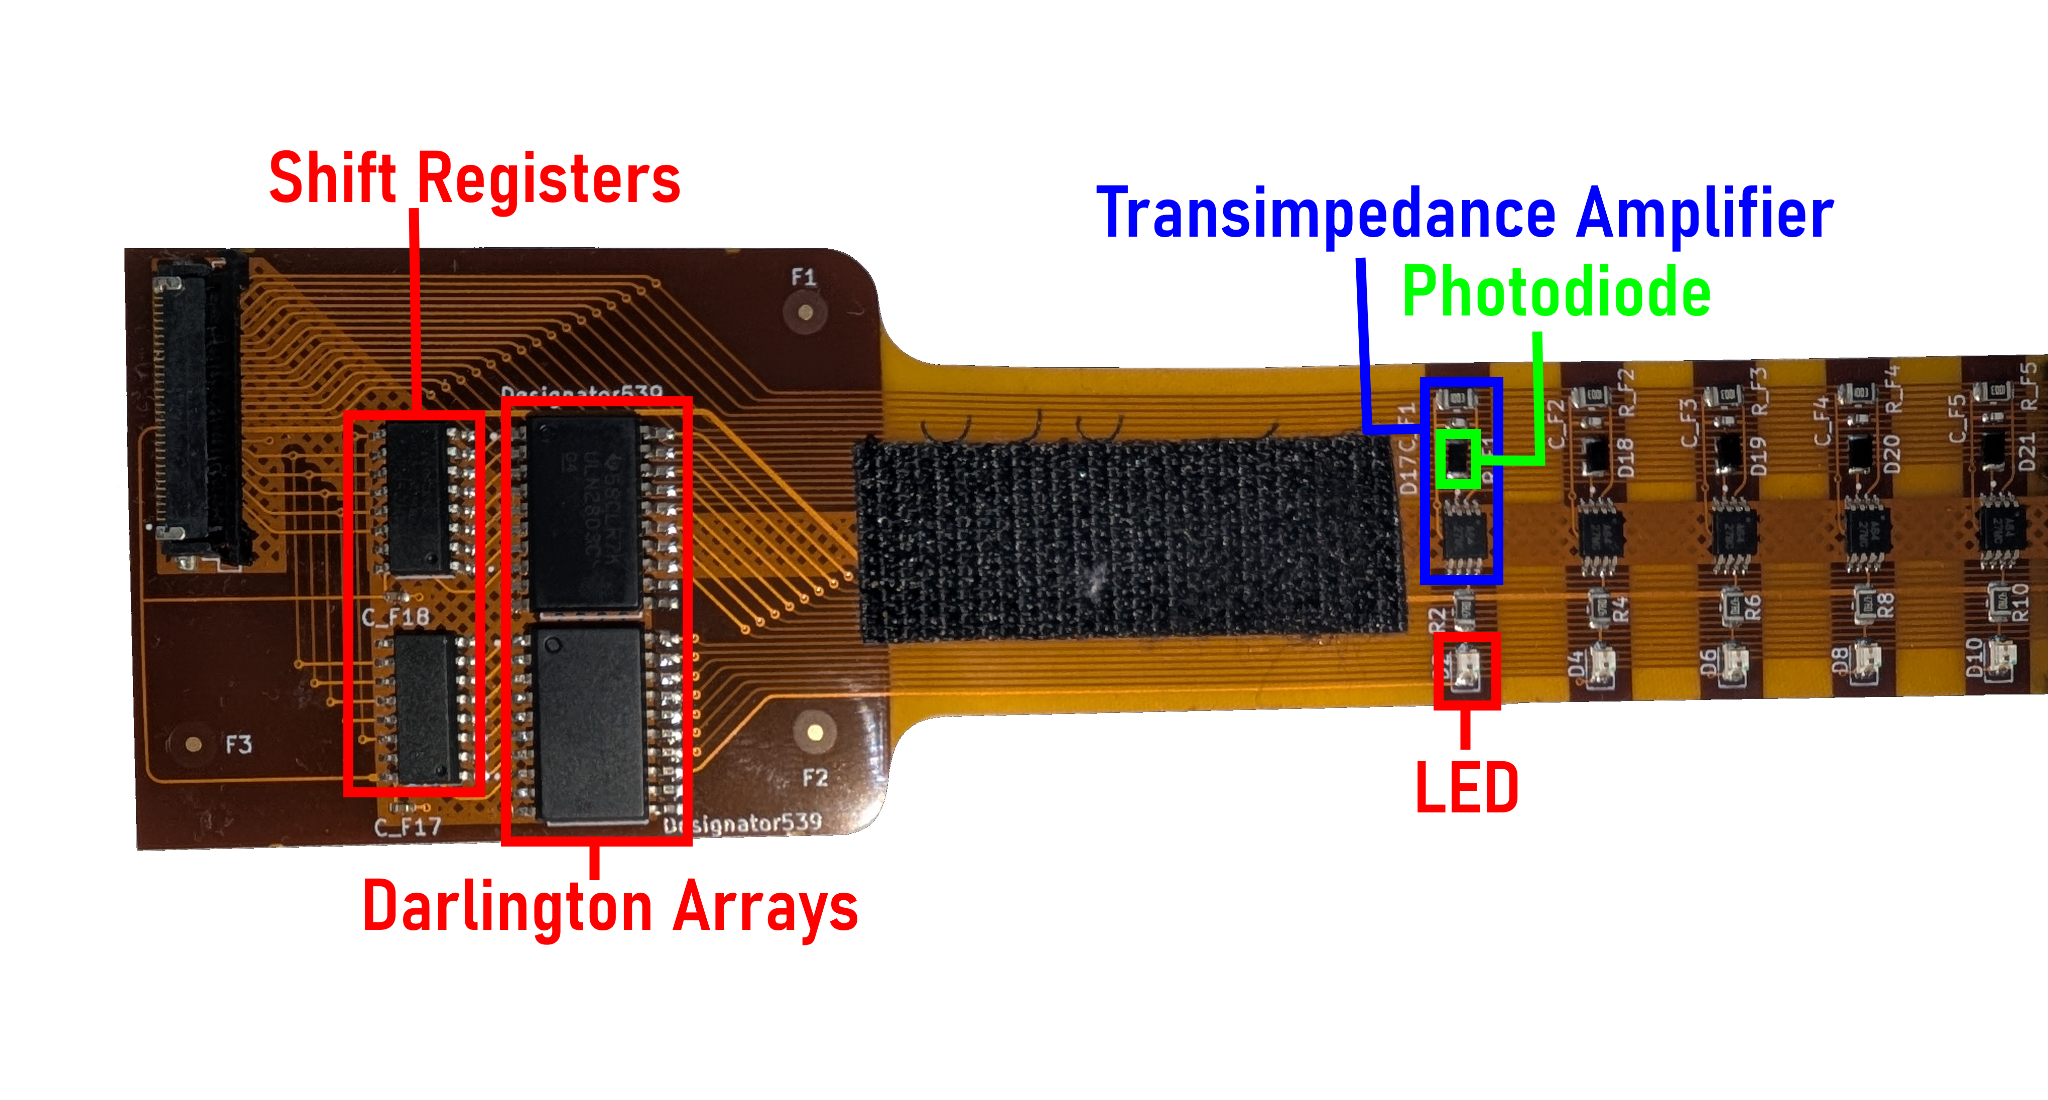
\includegraphics[width=0.8\linewidth]{FlexIR_design.png}
%     \caption{Design of the FlexIR wristband}
%     \label{fig:FlexIR}
% \end{figure}

% The wristband is based on a flexible PCB, shown in \autoref{fig:FlexIR}. There are two main sections: the head and the body.

% The head of the wristband contains two 74HC595D shift registers and two ULN2803C Darlington arrays which are used to drive the LEDs. It also contains an FFC connector, which is used to connect the device to a microcontroller.

% The main body of the wristband contains 16 stiffened segments. Each segment contains an LED, a photodiode and a transimpedance amplifier.

% Between the head and the body, there is a large empty section of the PCB which is used for fastening.

% \subsection{Fastening}
% Flexible PCBs cannot be stretched, so a mechanism is needed to fix the wristband in place once it is placed around a users wrist. The wrist circumference also varies significantly as users perform different hand gestures.

% An early prototype used a pin buckle, similar to a watch strap, to fasten the wristband. However, we found that due to the taper of the wrist, it was useful to fasten the ends of the wristband at a range of angles.

% Another prototype, shown in \autoref{fig:prototype}, consisted of a Velcro pad glued to a large empty section of the PCB and another pad glued to the stiffeners on the back. This allowed the wristband to fasten around any wrist thickness at any angle, but didn't accommodate for changes in wrist circumference throughout usage. 

% The final design uses one velco pad glued to a large empty section of the PCB, and another Velcro pad attached to an elastic strap, which is glued to the stiffeners on the back of the PCB. The wristband can be fastened tightly around the wrist, and has the ability to expand and constrict as the user performs gestures.

% \begin{figure}[htp]
%     \centering
%     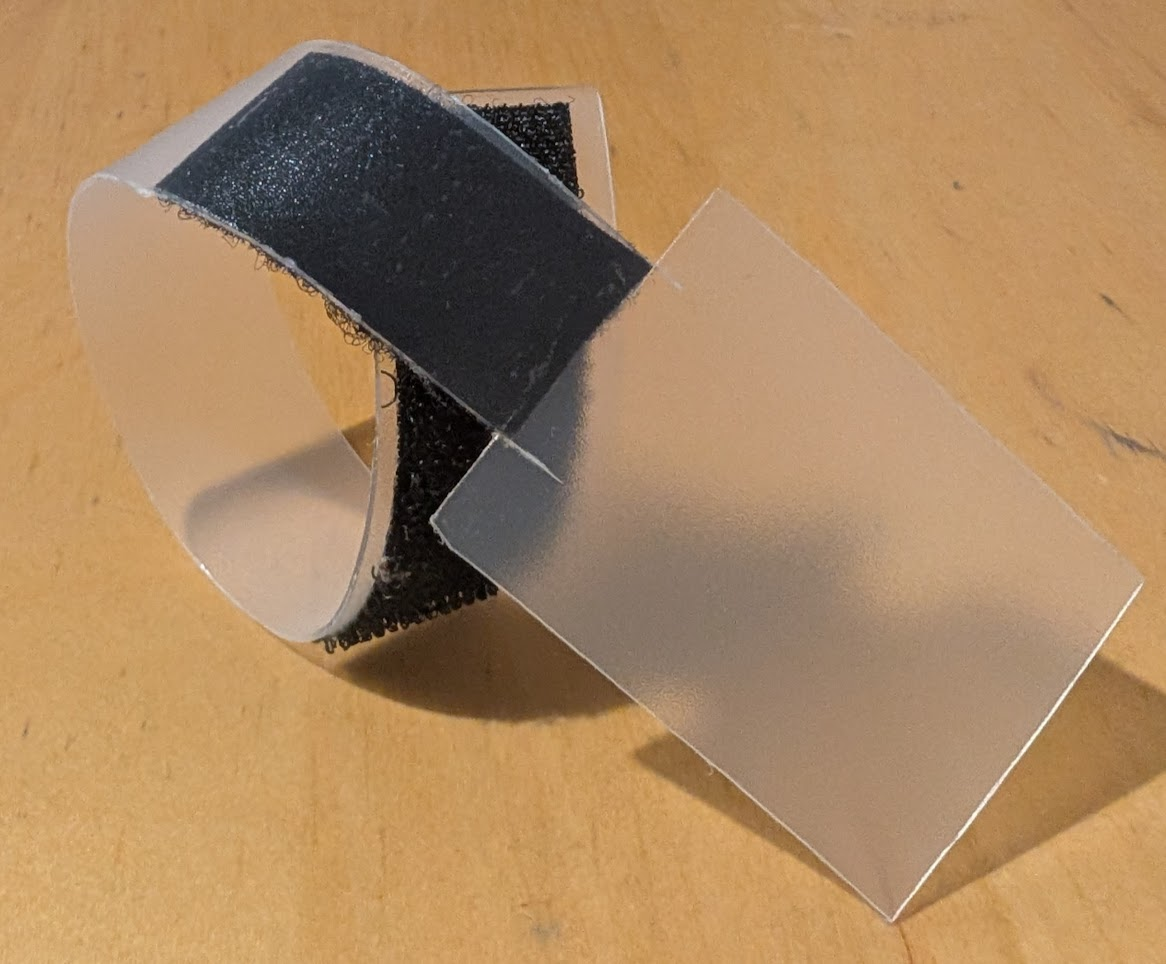
\includegraphics[width=0.33\linewidth]{FlexIR-prototype.jpg}
%     \caption{Initial prototype - the wristband can be fastened at an angle, accommodating for the natural taper of the wrist}
%     \label{fig:prototype}
% \end{figure}

% \section{PCB design}
% \subsection{Shift Registers}
% Each LED and photodiode must be individually controllable. To reduce the number of wires required between the wristband and microcontroller, we used 74HC595D shift registers for LED activation. Daisy chaining two 74HC595D chips allows for the control of 16 LEDs using 5 output pins of the microcontroller.
% \subsection{LED Circuit}
% The LED circuit consists of 16 pairs of LEDs and resistors. The microcontroller pins can't provide enough power to activate the LEDs, so we used ULN2803C Darlington arrays.P ower is supplied to the anode of each LED through a thick shared power trace running through the center of the PCB, and the cathode of each LED is connected to an output of a ULN2803C. When an input on one of the ULN2803C chips is activated, the corresponding output is connected to ground, and current flows through the LED. The inputs of the ULN2803Cs are activated by the outputs of two 74HC595D shift registers.
% \subsection{Photodiode Circuit}
% The photodiode circuit is made up of 16 photodiodes, each connected to a transimpedance amplifier. The photodiode circuit is connected to power through the shared central power trace, and is grounded through a large ground plane on the back of the PCB. The transimpedance amplifiers convert the small current produced by the photodiodes into larger voltages that can be read by the microcontroller. They each contain an opamp, a 100k resistor and a 1pF capacitor.

% \section{LED/Photodiode Selection}
% We chose to investigate the effect of LED viewing angle on classification accuracy. We selected two LEDs with similar forward voltages and the same total radiant power, but different viewing angles (and radiant intensities).


% We hypothesize that:
% \begin{itemize}
%     \item LEDs with smaller viewing angles will be more effective at penetrating the wrist due to their higher radiant intensity, producing higher quality measurements at photodiodes opposite the active LED.
%     \item While LEDs with smaller viewing angles will be less effective at penetrating the wrist, the scattering and reflection of light against tendons close to the surface of the wrist will be more apparent, leading to better results from photodiodes adjacent to the active LED.
% \end{itemize}

% The selected LEDs had to satsify the following constraints:

% \begin{itemize}
%     \item Constrasting viewing angle
%     \item Similar radiant power
%     \item Small SMD package
% \end{itemize}

% The LEDs selected were:
% \begin{itemize}
%     \item The \textbf{VSMB1940X01}, with a $\pm 60^\circ$ viewing angle.
%     \item The \textbf{TSML1020}, with a $\pm 12^\circ$ viewing angle.
% \end{itemize}

% Both LEDs have the same current-voltage graphs and the same radiant power (40 mW at 100 mA). Since they are both powered from the same 3.3 V pin on the Teensy, this means they draw the same amount of current and produce the same amount of light energy. The TSML1020 has a much smaller viewing angle of $\pm 12^\circ$, so the radiant intensity is higher, as shown in \autoref{fig:viewing_angle}.

% \begin{figure}[htp]
%     \centering
%     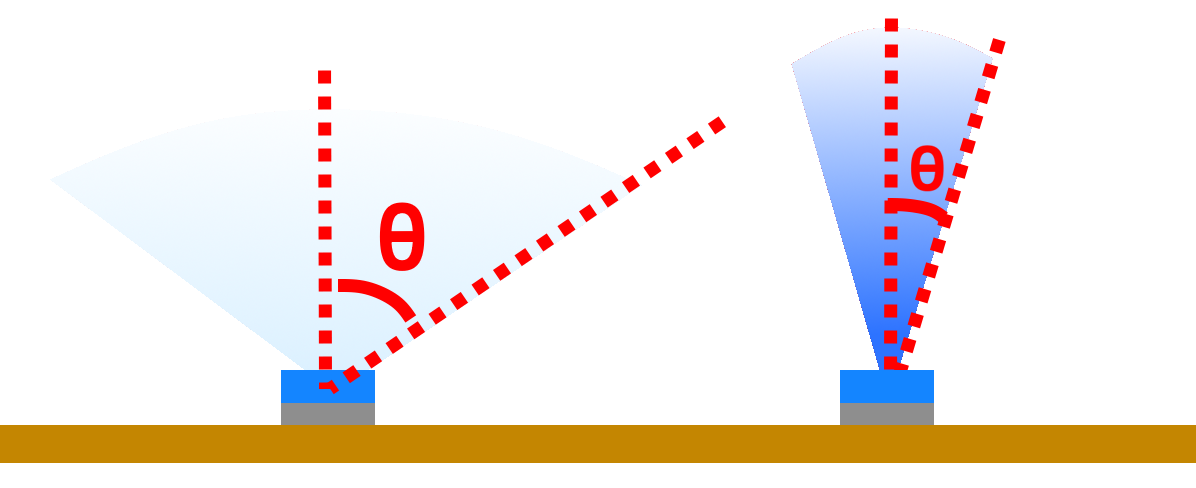
\includegraphics[width=0.6\linewidth]{ViewingAngle.png}
%     \caption{LEDs with the same radiant power and different viewing angles have different radiant intensities}
%     \label{fig:viewing_angle}
% \end{figure}

% Both LEDs emit 940 nm wavelength light. Although GestIR identified 860 nm LEDs as particularly effective and 950 nm less effective due to absorption peaks in lipids around 930 nm, the chosen LEDs were the only available options with consistent wavelengths that satisfied the constraints. 950 nm was still shown to be effective, achieving 85.8\% accuracy.

% -----------------------------------------------------------------------------

\chapter{Viewing Angle Experiment}
\label{chapter:experiment}
In this chapter, we compare the impact of the LED viewing angle on the effectiveness of gesture 
classification. We capture gesture data using LEDs with a narrow viewing angle ($\pm 12^\circ$ and 
$\pm 60^\circ$).

Like GestIR \cite{diamand2025}, the 20 gestures used were drawn from the HaGRID (HAnd Gesture
Recognition Image Dataset) \cite{Alexander2024HaGRIDDataset} and SensIR \cite{McIntosh2017SensIR:Reflection}. The gesture set has a range of very distinct gestures with large wrist movements, and more subtle gestures, e.g pinch variations.

\begin{table}[ht]
    \centering
    \small
    \setlength{\tabcolsep}{4pt}
    \renewcommand{\arraystretch}{1.2} 
    
    \resizebox{0.75\textwidth}{!}{%
    \begin{minipage}{0.48\textwidth}
        % Column definitions with integrated centering and backslash fix
        \begin{tabular}{|>{\centering\arraybackslash}m{2.2cm}|>{\centering\arraybackslash}m{1.8cm}|>{\centering\arraybackslash}m{1.8cm}|}
            \hline
            \textbf{Name} & \textbf{Above View} & \textbf{Side View} \\ \hline
            Pinch Index & 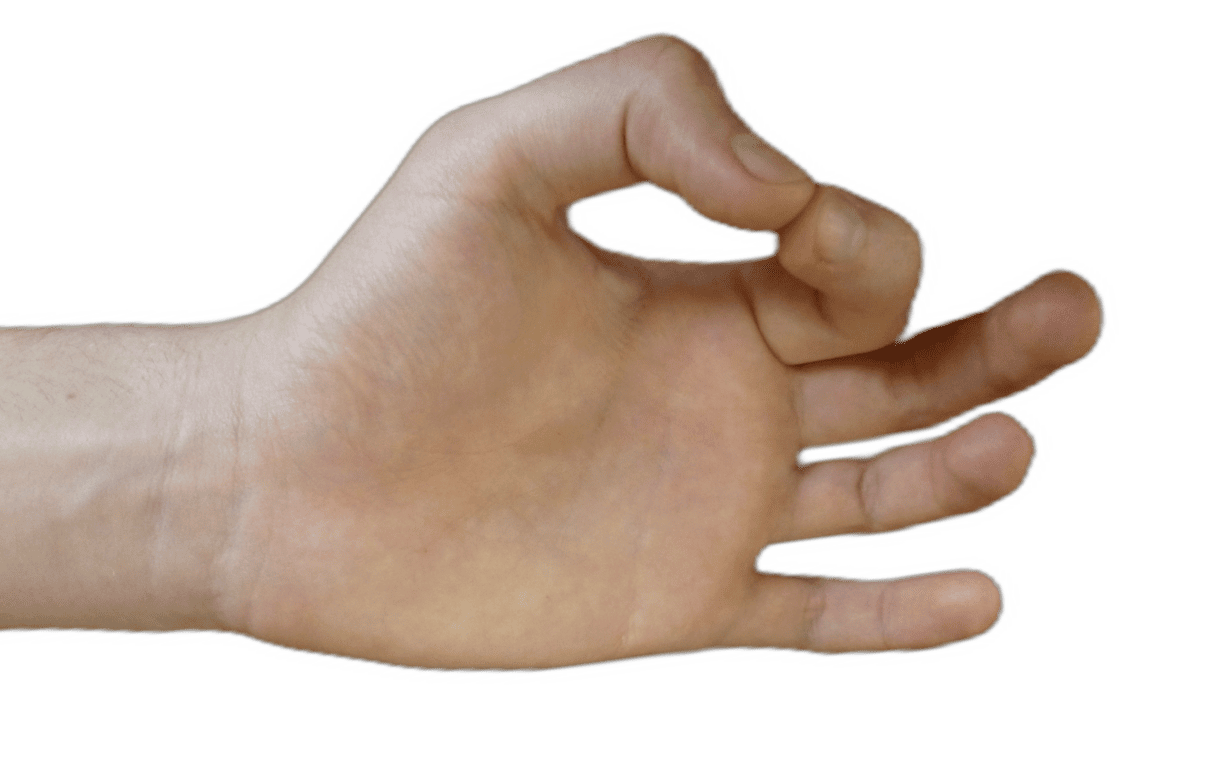
\includegraphics[width=\linewidth]{gesture_images/pinch_index_above.png} & 
\includegraphics[width=\linewidth]{gesture_images/pinch_index_side.png} \\ \hline
            Pinch Middle & 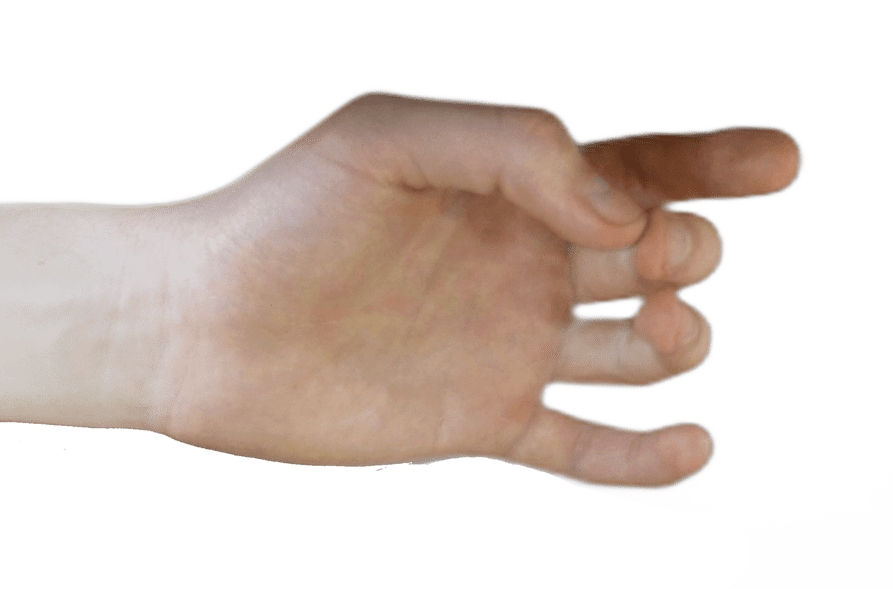
\includegraphics[width=\linewidth]{gesture_images/pinch_middle_above.png} & 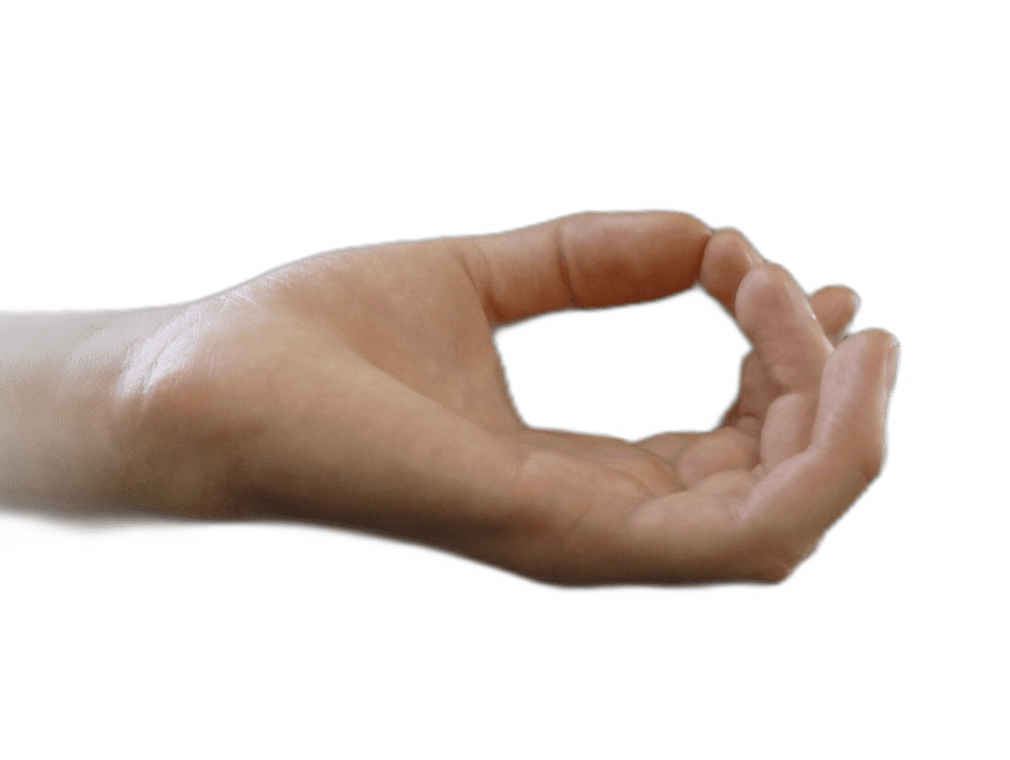
\includegraphics[width=\linewidth]{gesture_images/pinch_middle_side.png} \\ \hline
            Pinch Ring & 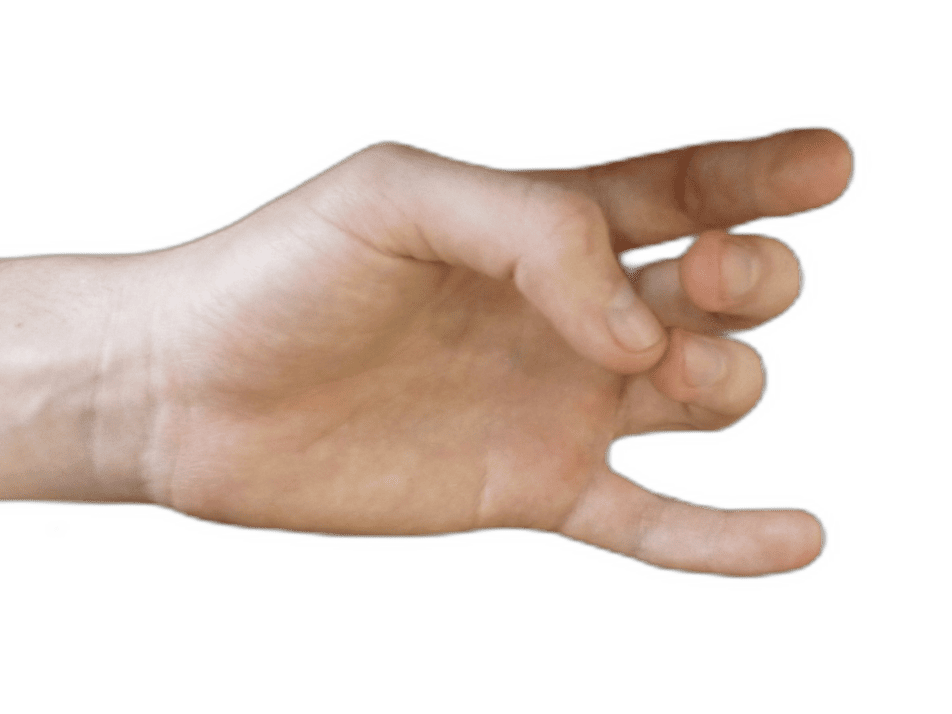
\includegraphics[width=\linewidth]{gesture_images/pinch_ring_above.png} & 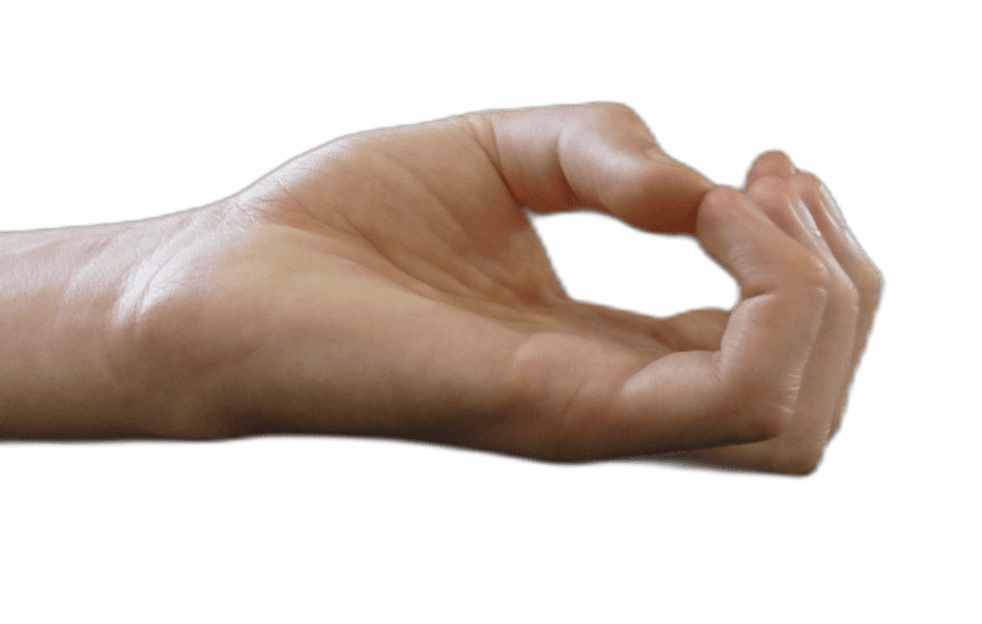
\includegraphics[width=\linewidth]{gesture_images/pinch_ring_side.png} \\ \hline
            Pinch Pinkie & 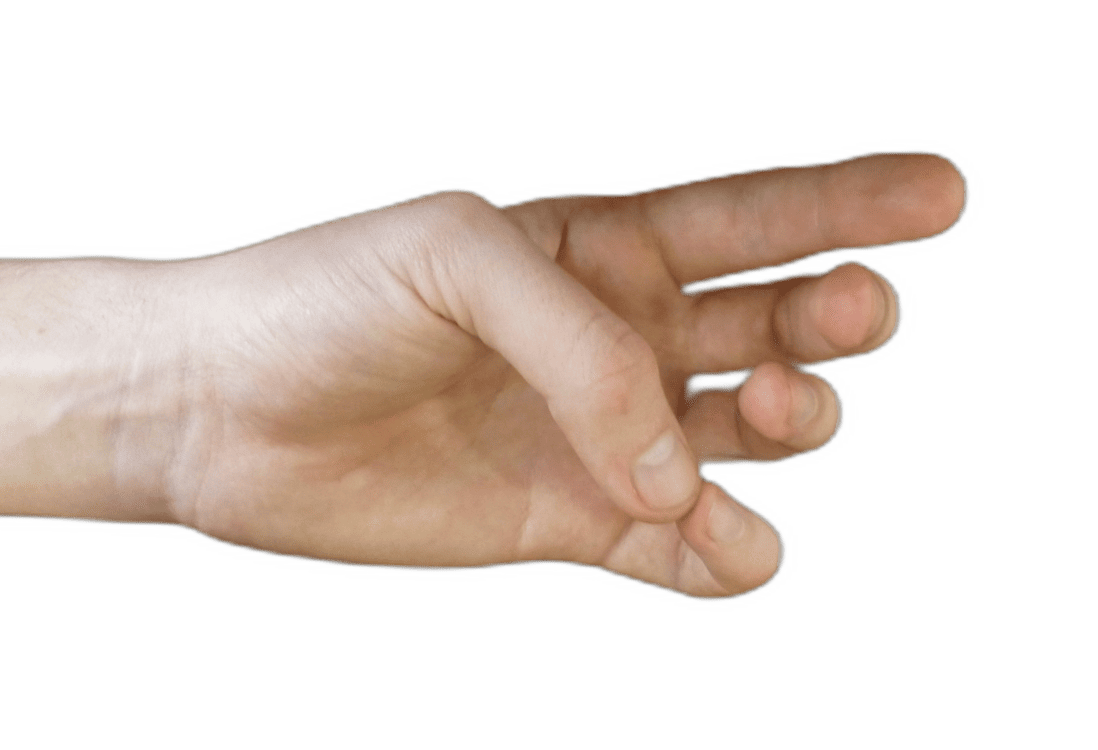
\includegraphics[width=\linewidth]{gesture_images/pinch_pinkie_above.png} & 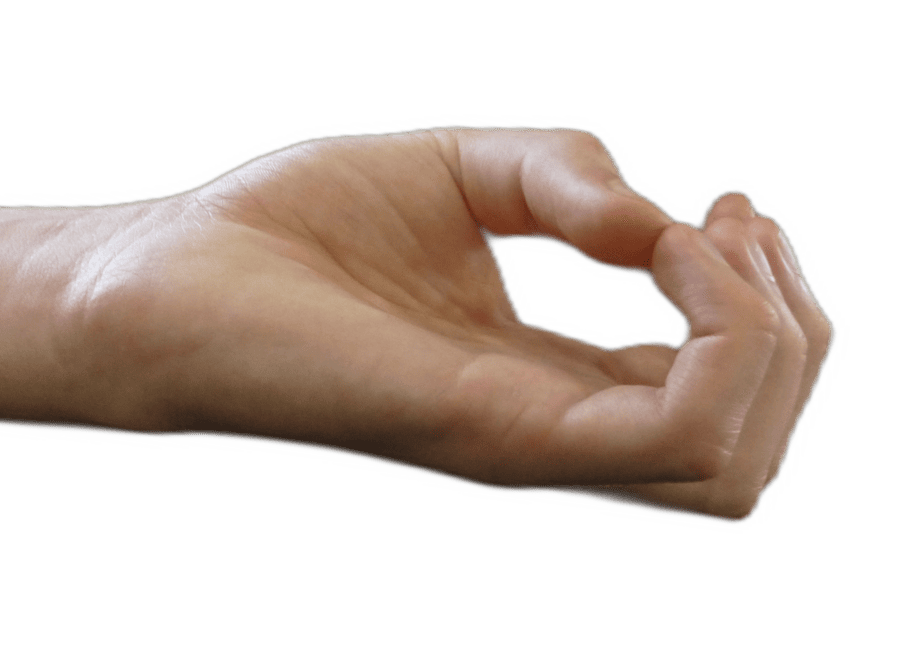
\includegraphics[width=\linewidth]{gesture_images/pinch_pinkie_side.png} \\ \hline
            Like & 
\includegraphics[width=\linewidth]{gesture_images/like_above.png} & 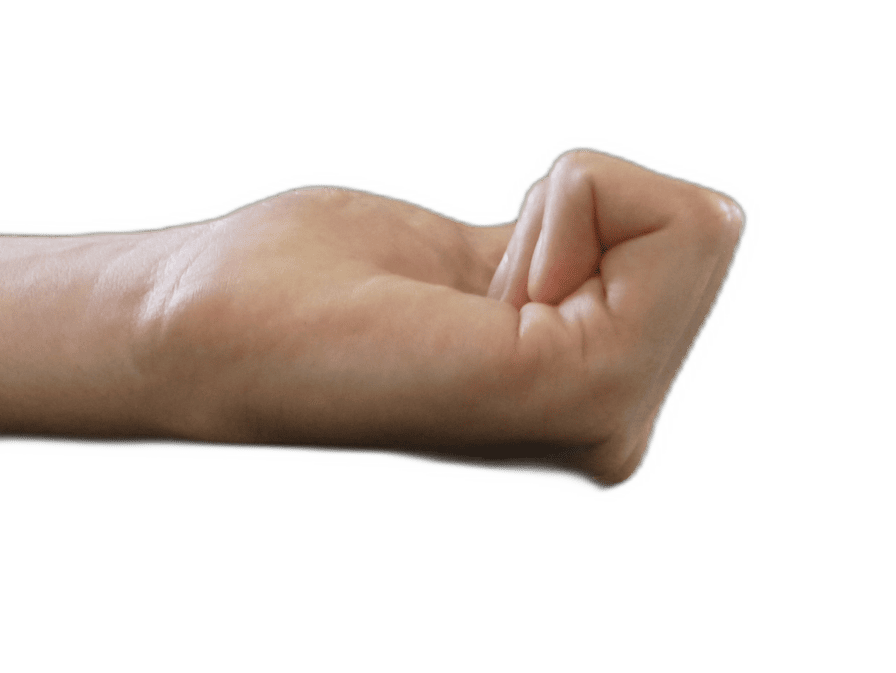
\includegraphics[width=\linewidth]{gesture_images/like_side.png} \\ \hline
            One & 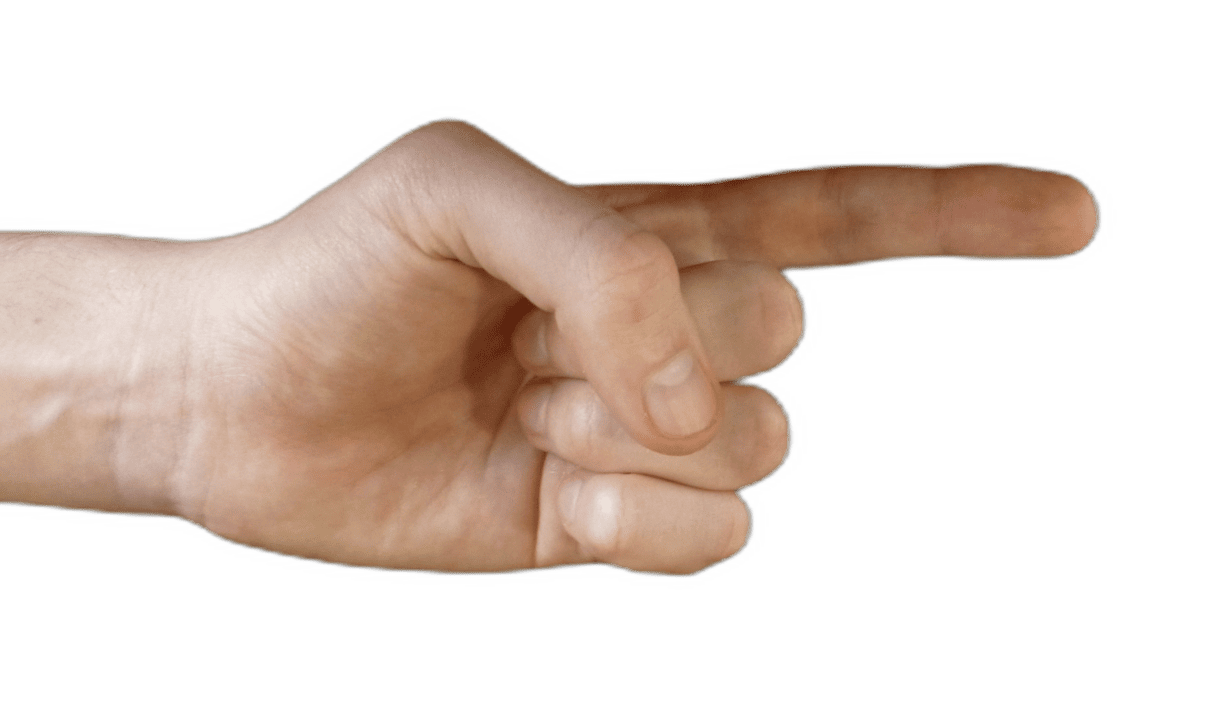
\includegraphics[width=\linewidth]{gesture_images/one_above.png} & 
\includegraphics[width=\linewidth]{gesture_images/one_side.png} \\ \hline
            Middle & 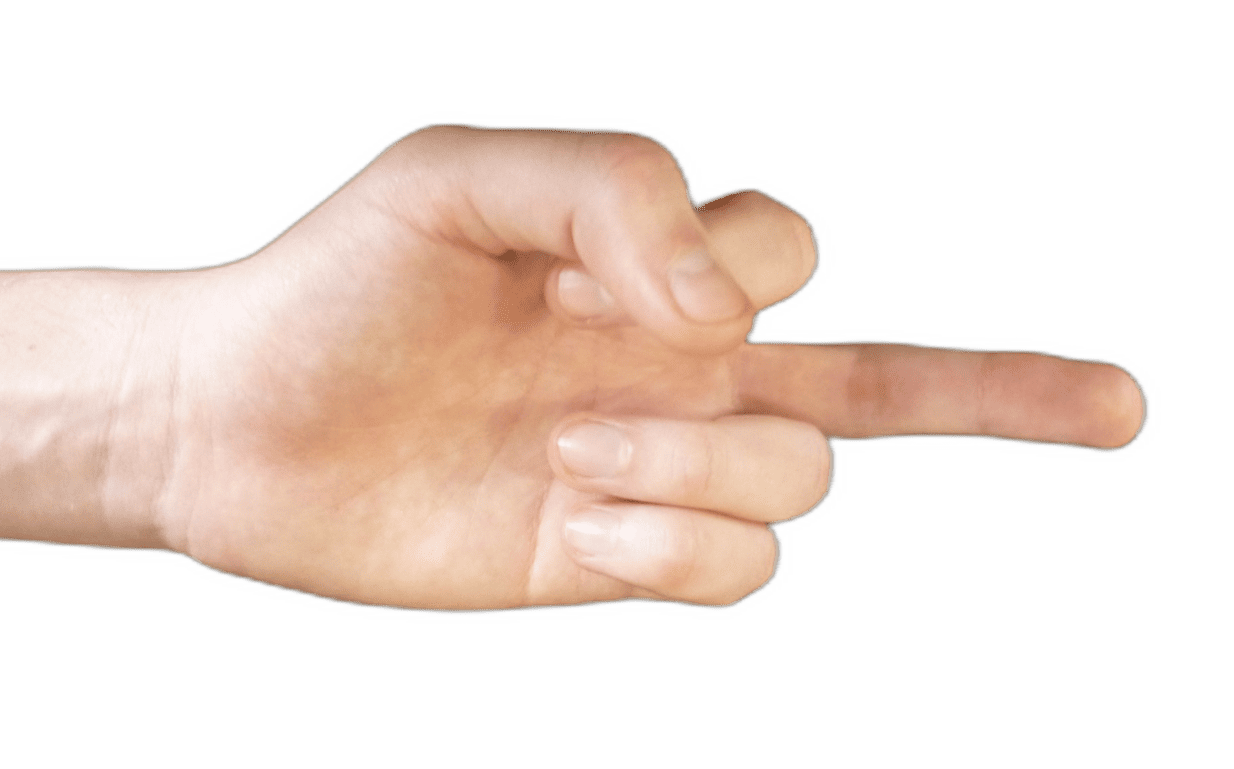
\includegraphics[width=\linewidth]{gesture_images/middle_above.png} & 
\includegraphics[width=\linewidth]{gesture_images/middle_side.png} \\ \hline
            Two & 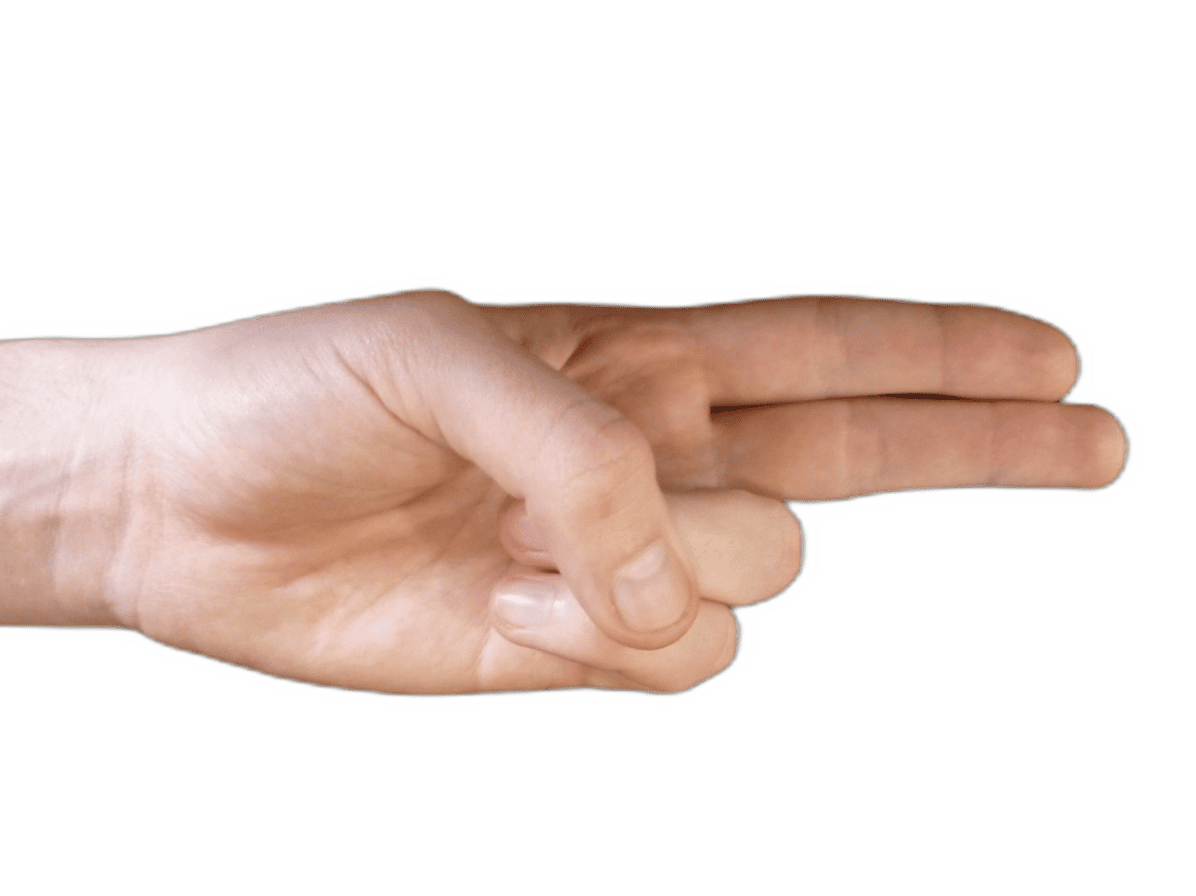
\includegraphics[width=\linewidth]{gesture_images/two_above.png} & 
\includegraphics[width=\linewidth]{gesture_images/two_side.png} \\ \hline
            Gun & 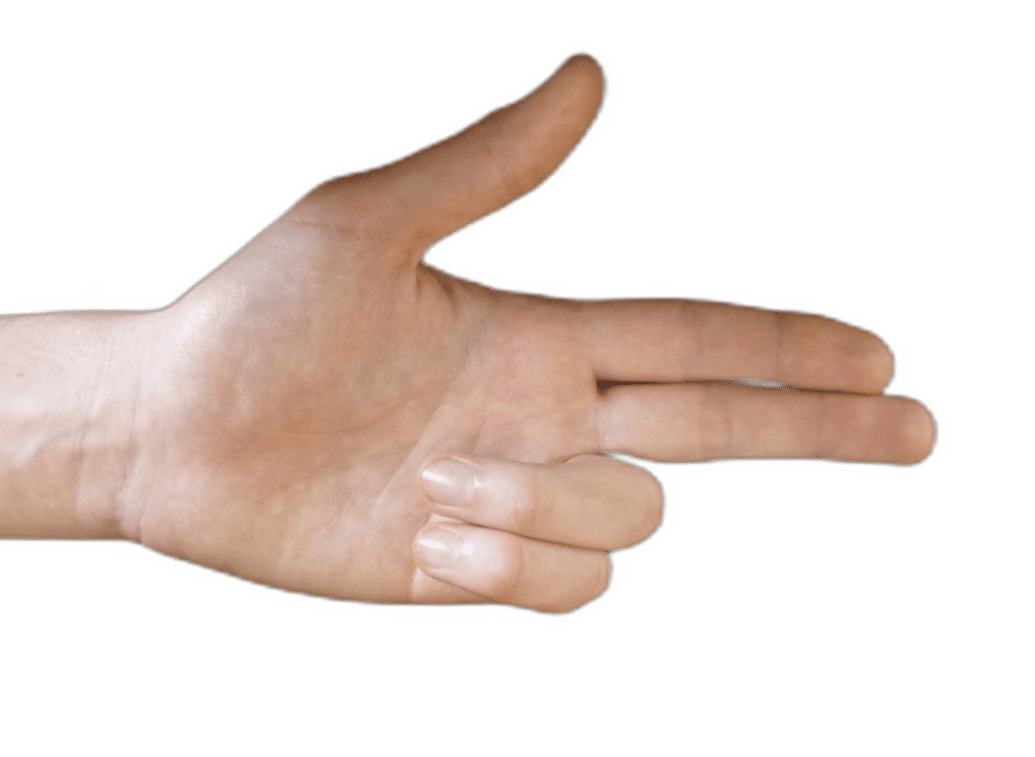
\includegraphics[width=\linewidth]{gesture_images/gun_above.png} & 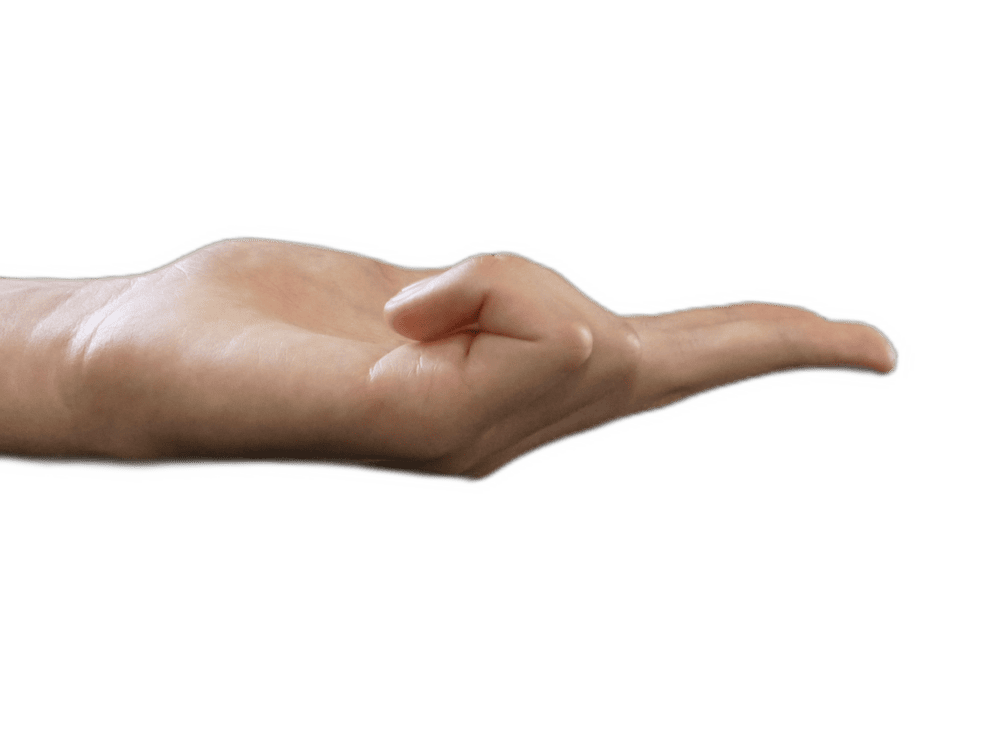
\includegraphics[width=\linewidth]{gesture_images/gun_side.png} \\ \hline
            Rock & 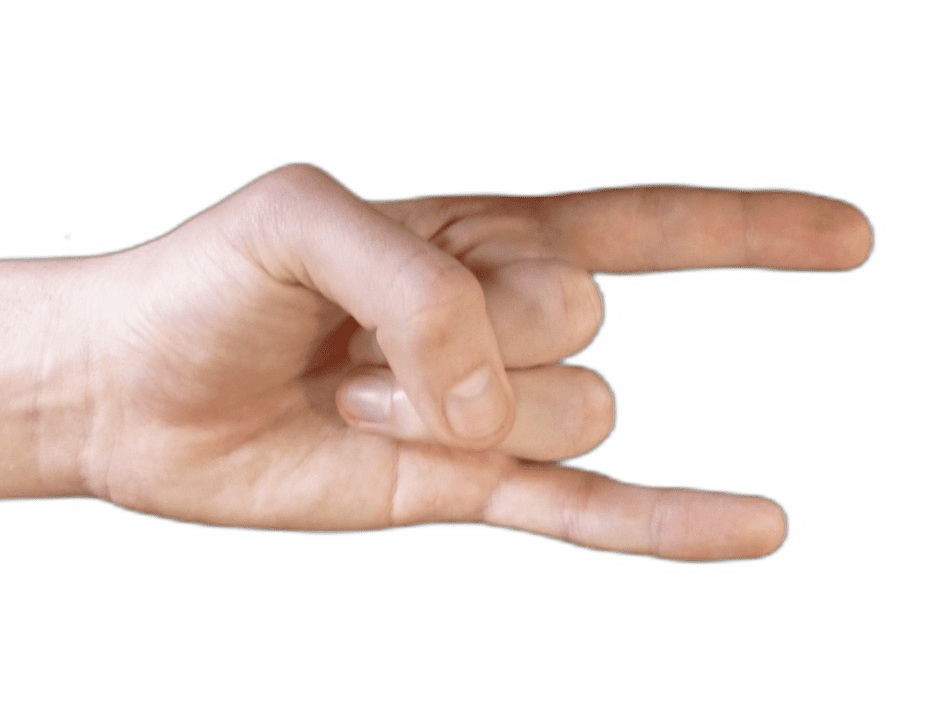
\includegraphics[width=\linewidth]{gesture_images/rock_above.png} & 
\includegraphics[width=\linewidth]{gesture_images/rock_side.png} \\ \hline
        \end{tabular}
    \end{minipage}
    \hfill 
    \begin{minipage}{0.48\textwidth}
        \begin{tabular}{|>{\centering\arraybackslash}m{2.2cm}|>{\centering\arraybackslash}m{1.8cm}|>{\centering\arraybackslash}m{1.8cm}|}
            \hline
            \textbf{Name} & \textbf{Above View} & \textbf{Side View} \\ \hline
            Stop Right & 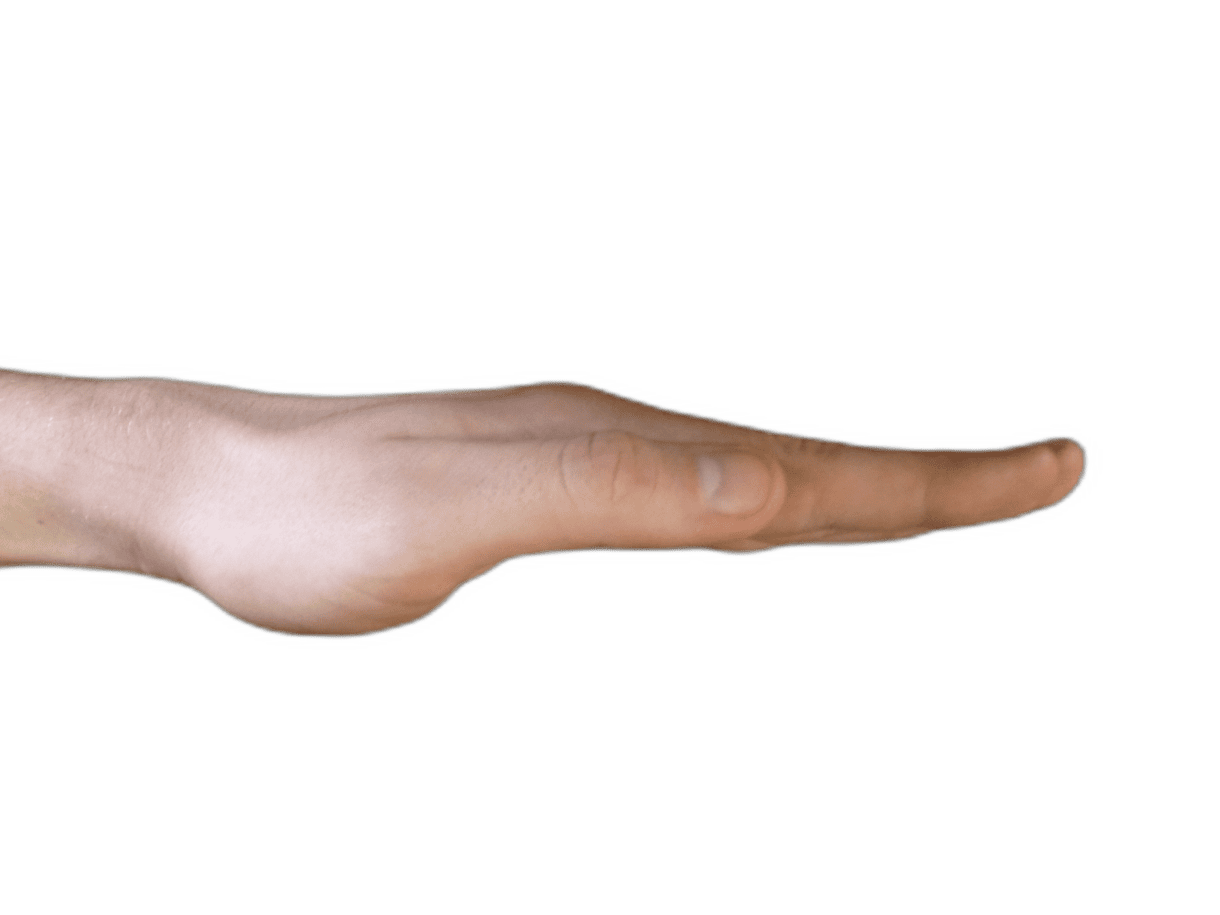
\includegraphics[width=\linewidth]{gesture_images/stop_right_above.png} & 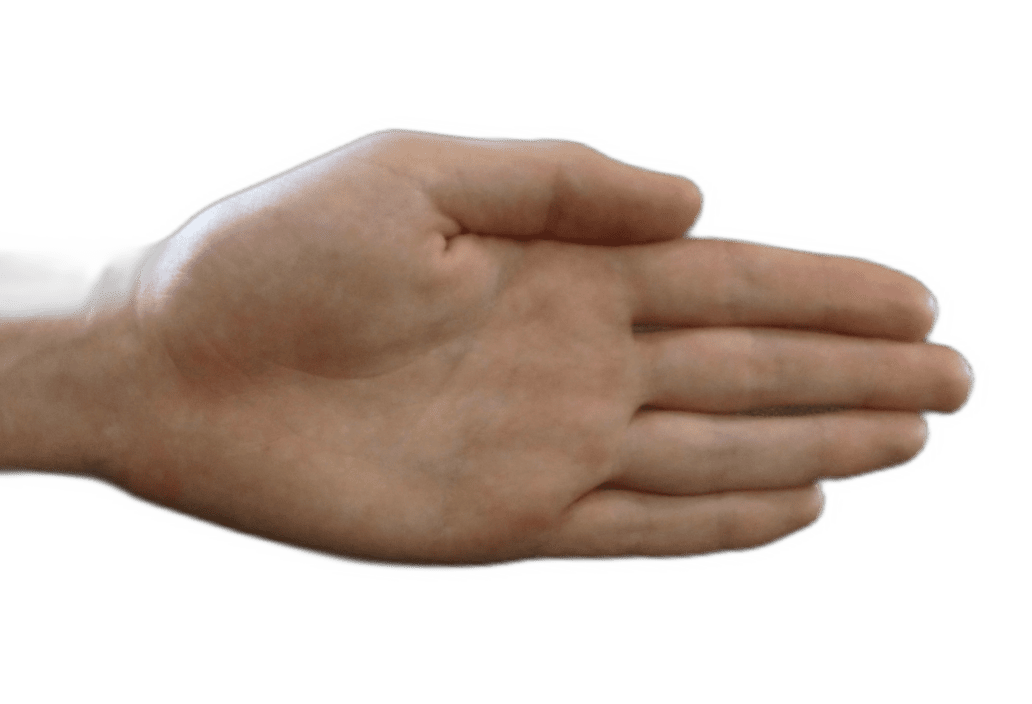
\includegraphics[width=\linewidth]{gesture_images/stop_right_side.png} \\ \hline
            Stop Down & 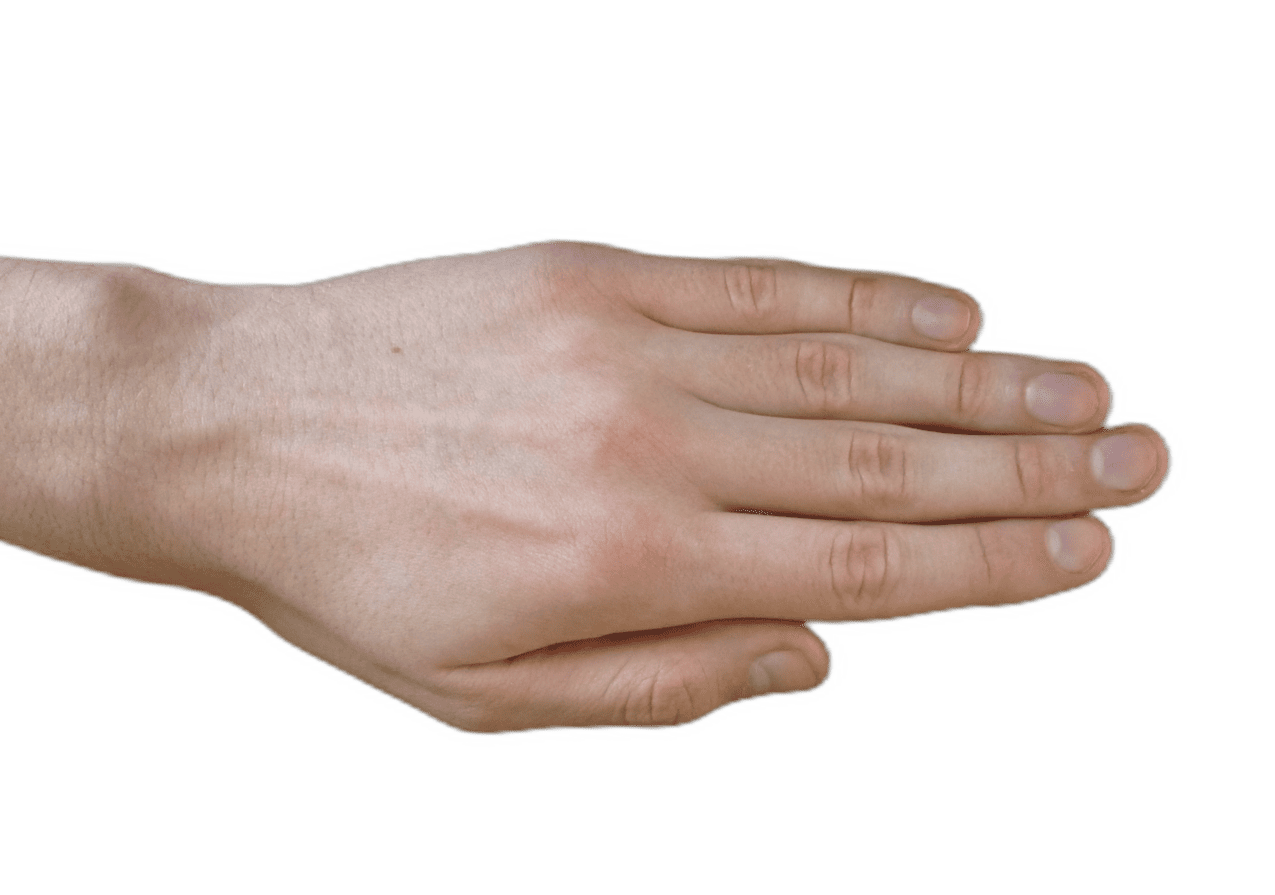
\includegraphics[width=\linewidth]{gesture_images/stop_down_above.png} & 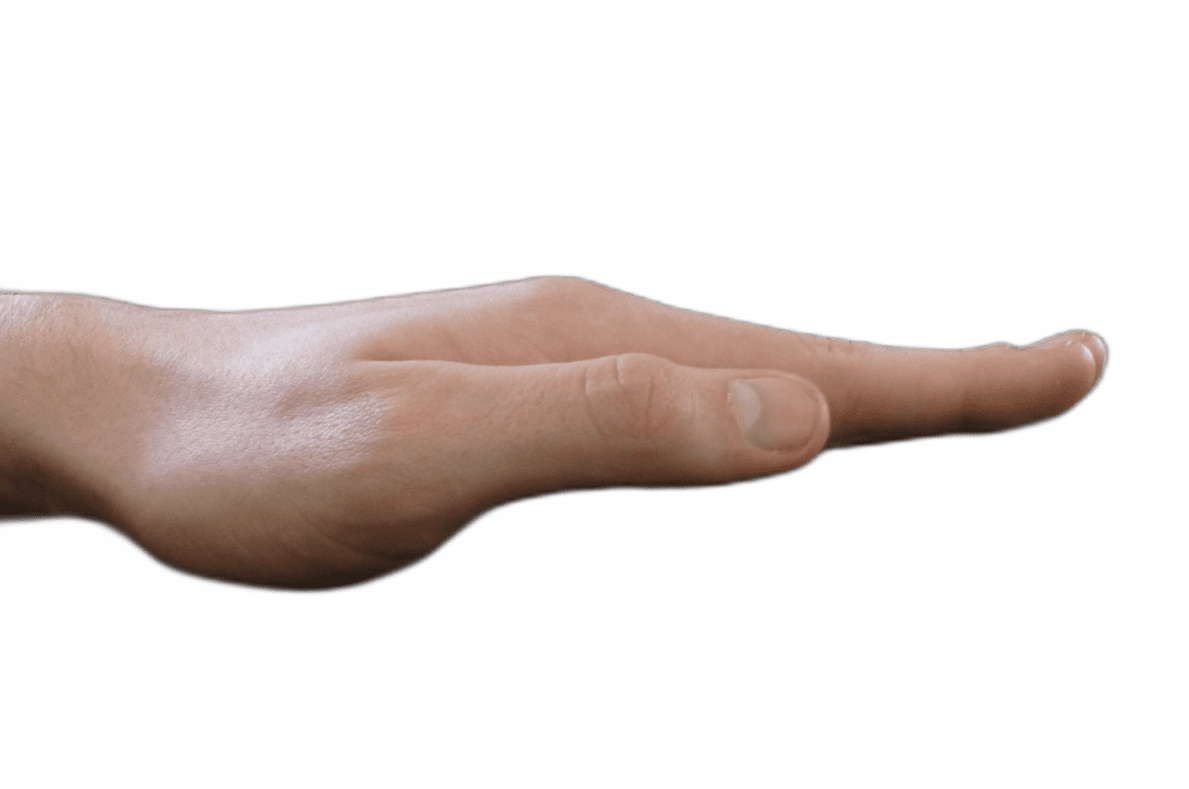
\includegraphics[width=\linewidth]{gesture_images/stop_down_side.png} \\ \hline
            Stop Up & 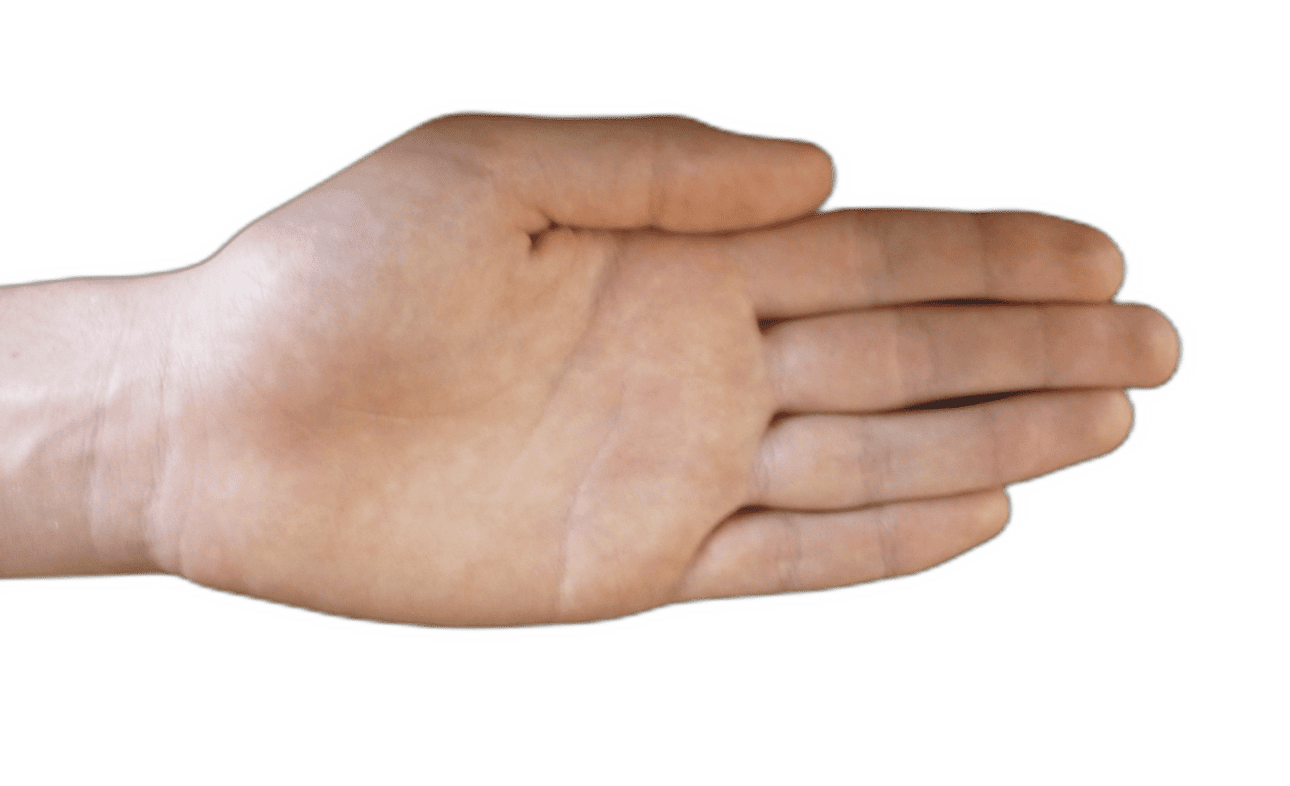
\includegraphics[width=\linewidth]{gesture_images/stop_up_above.png} & 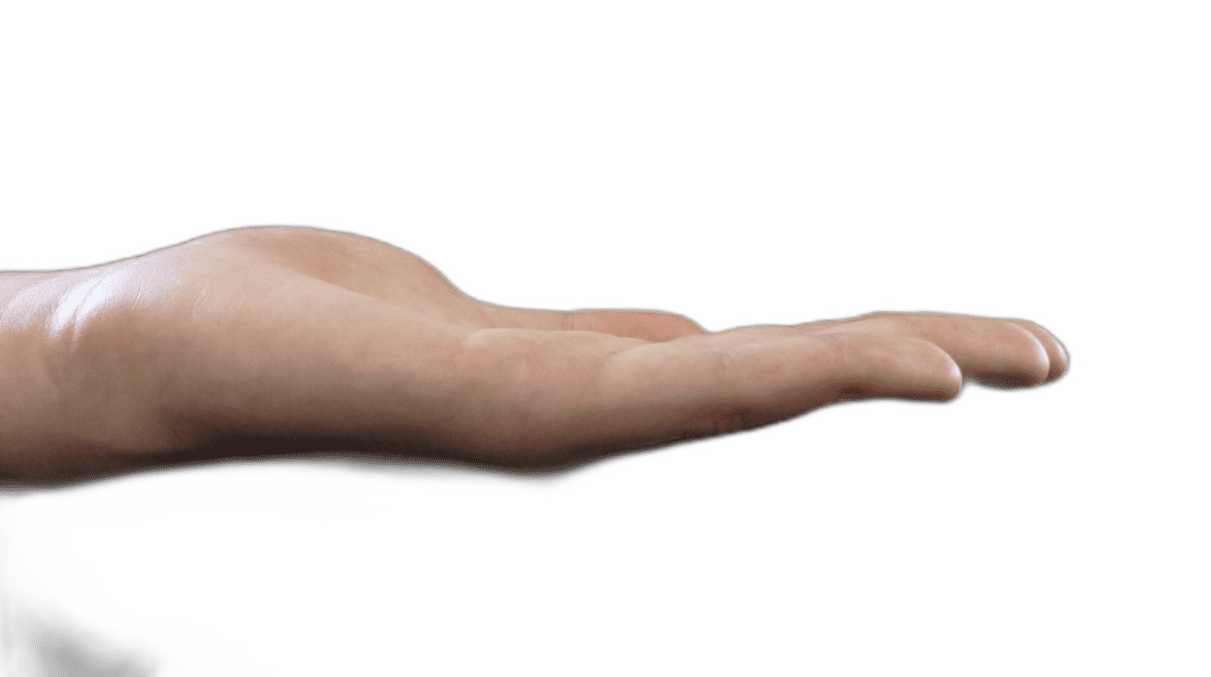
\includegraphics[width=\linewidth]{gesture_images/stop_up_side.png} \\ \hline
            Spread Right & 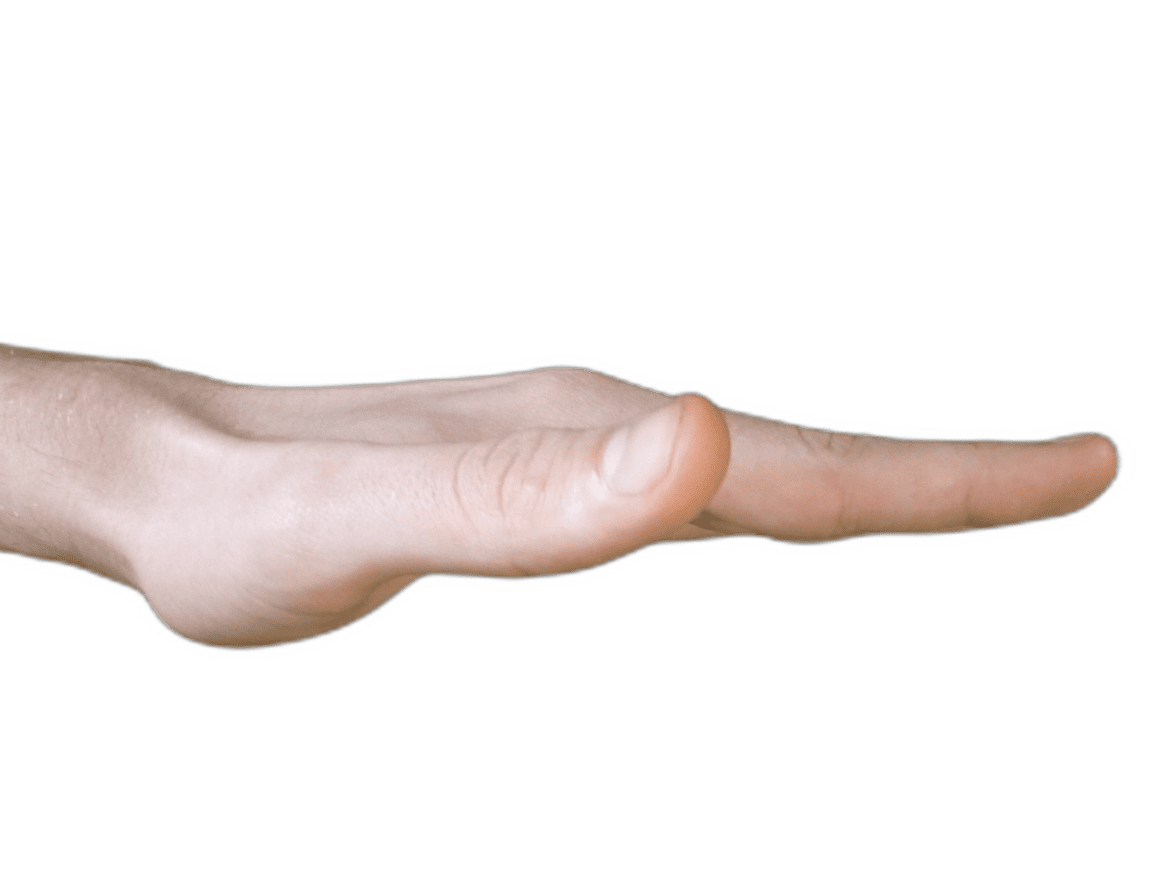
\includegraphics[width=\linewidth]{gesture_images/spread_right_above.png} & 
\includegraphics[width=\linewidth]{gesture_images/spread_right_side.png} \\ \hline
            Spread Down & 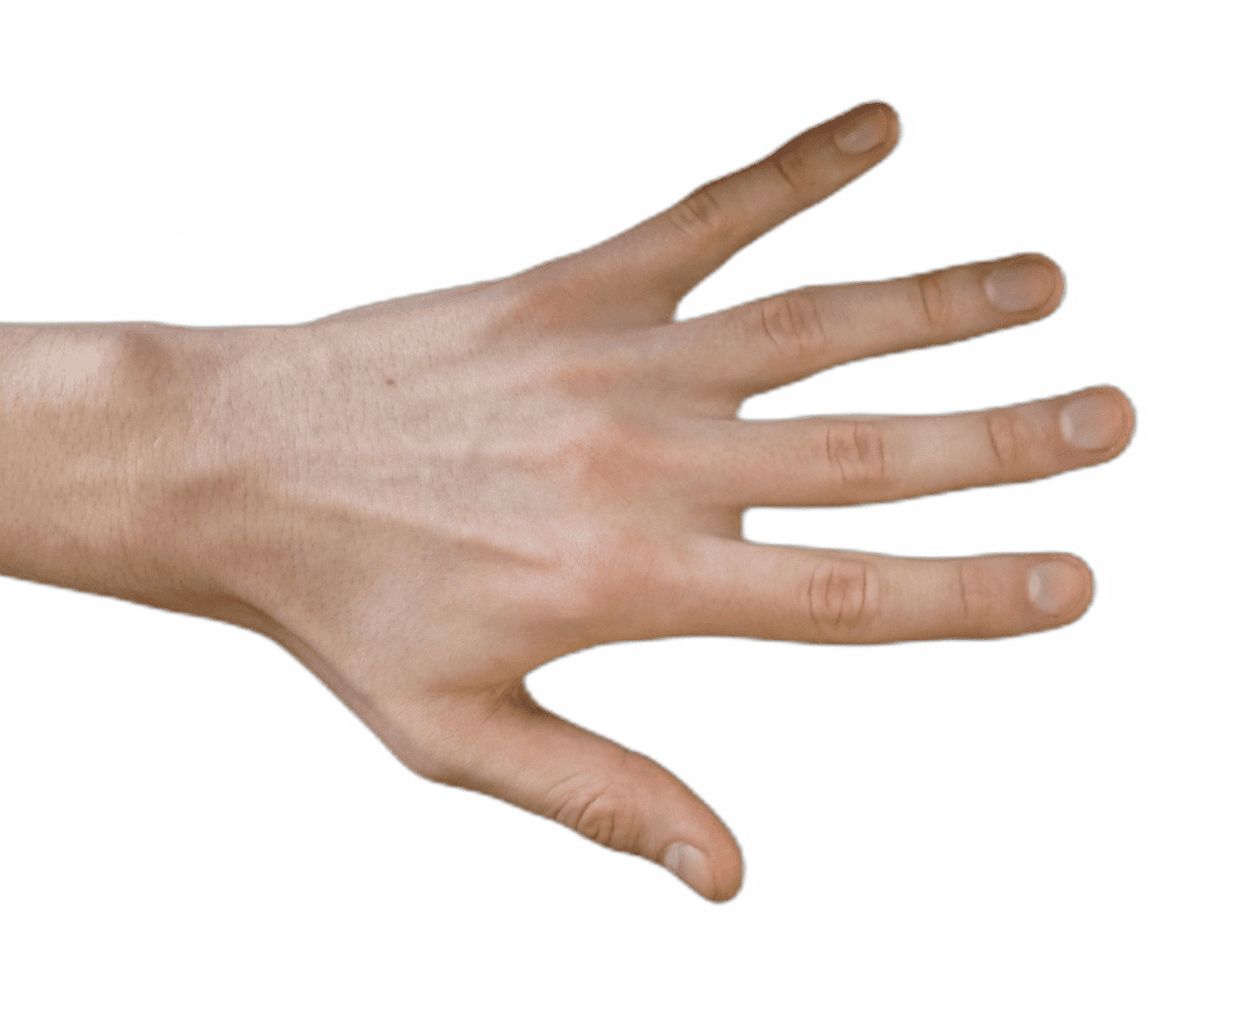
\includegraphics[width=\linewidth]{gesture_images/spread_down_above.png} & 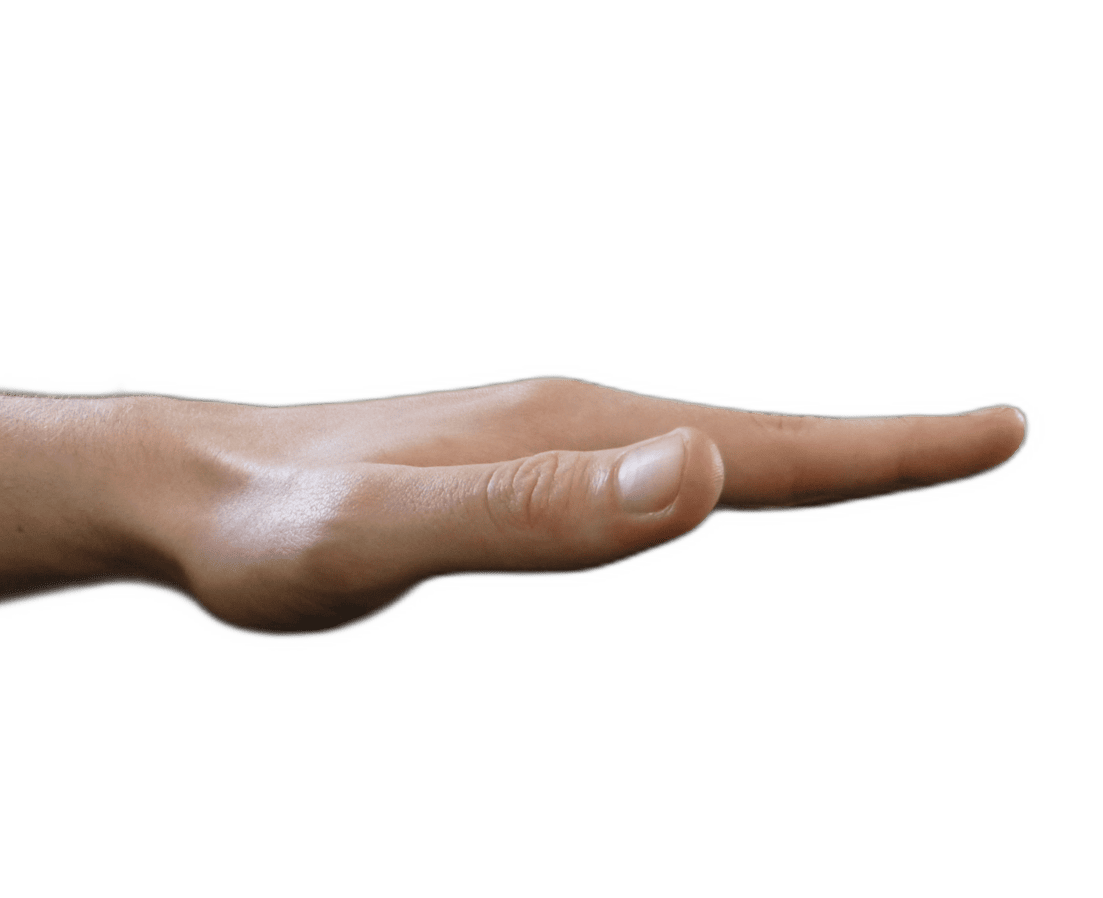
\includegraphics[width=\linewidth]{gesture_images/spread_down_side.png} \\ \hline
            Spread Up & 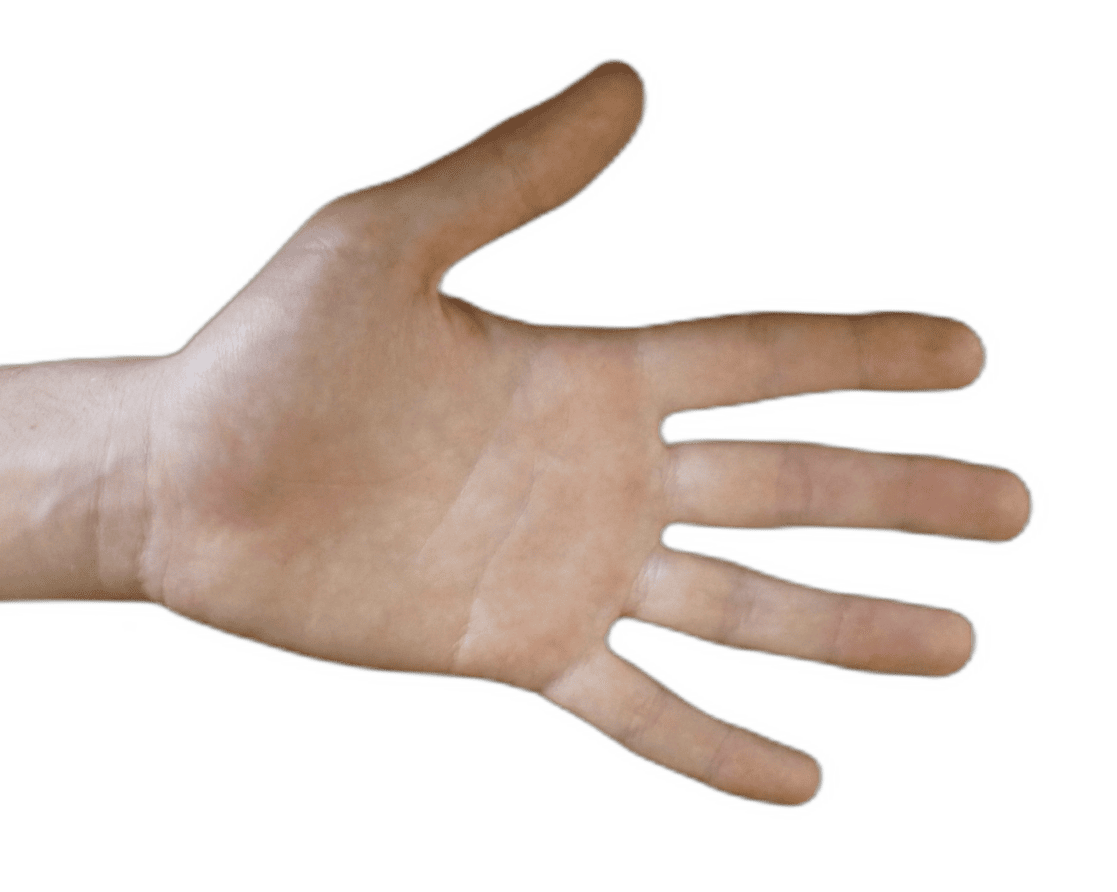
\includegraphics[width=\linewidth]{gesture_images/spread_up_above.png} & 
\includegraphics[width=\linewidth]{gesture_images/spread_up_side.png} \\ \hline
            Grabbing & 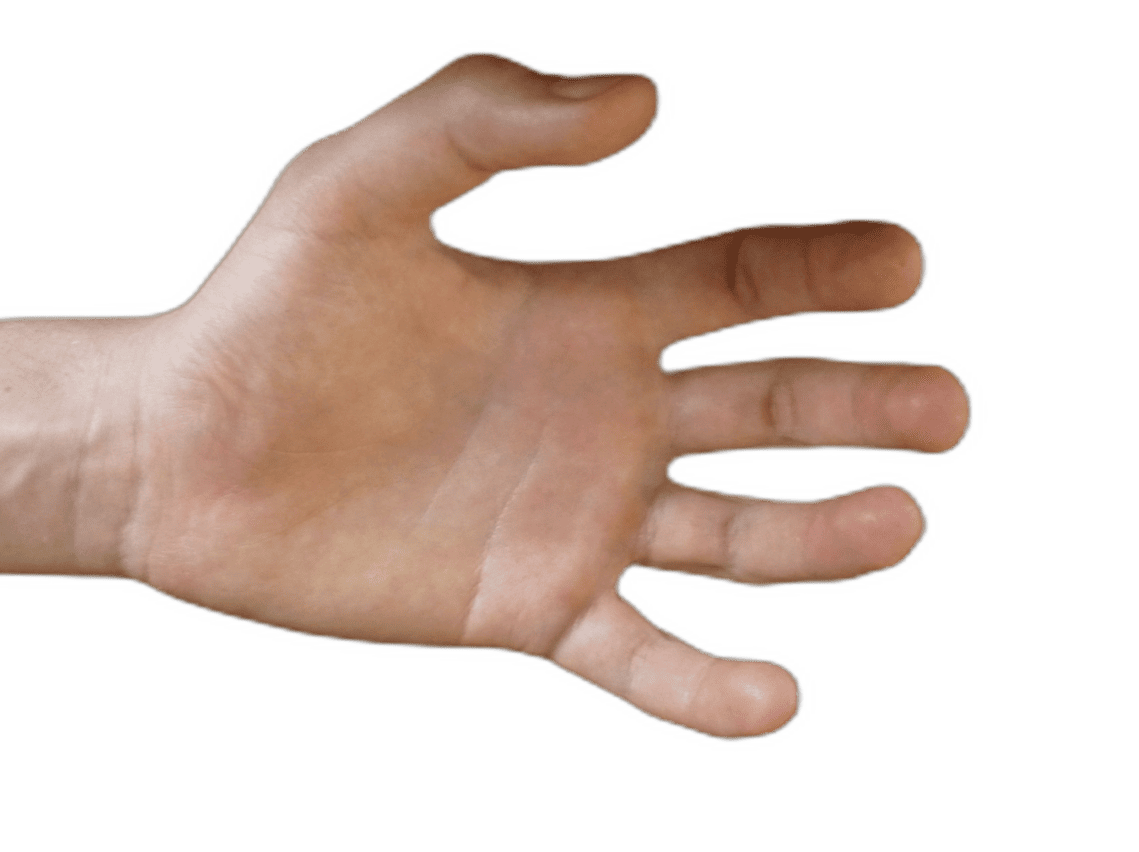
\includegraphics[width=\linewidth]{gesture_images/grabbing_above.png} & 
\includegraphics[width=\linewidth]{gesture_images/grabbing_side.png} \\ \hline
            Extension & 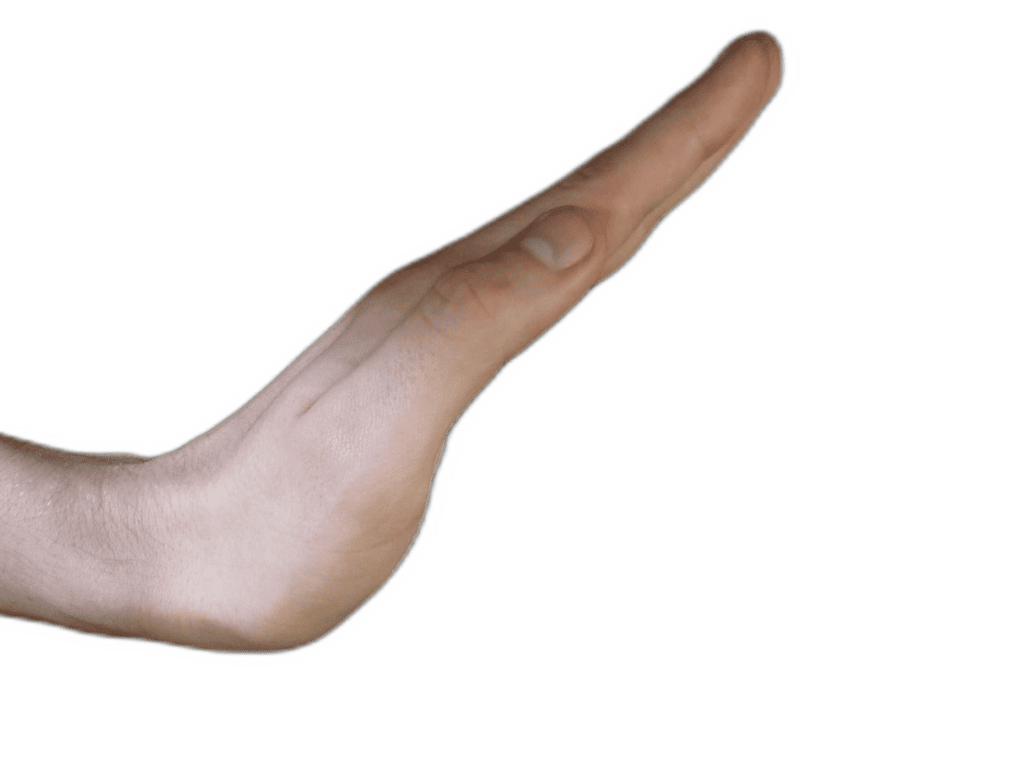
\includegraphics[width=\linewidth]{gesture_images/extension_above.png} & 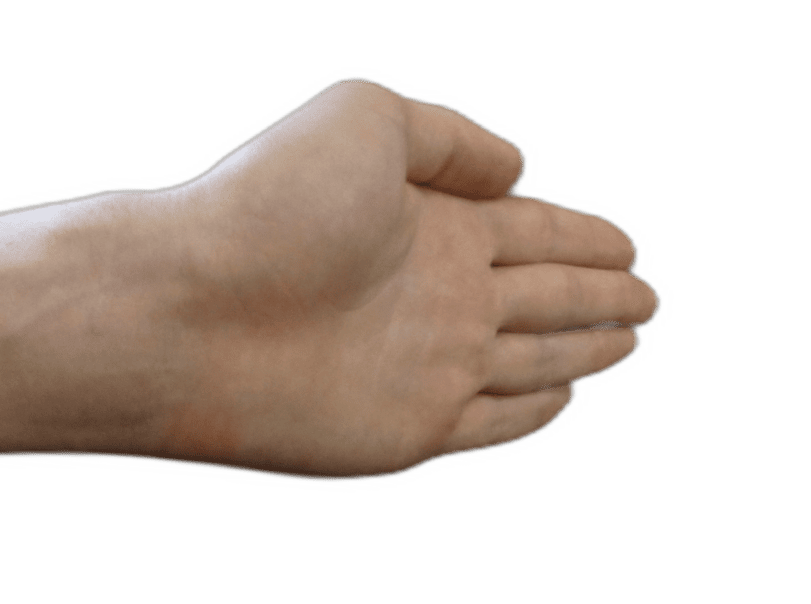
\includegraphics[width=\linewidth]{gesture_images/extension_side.png} \\ \hline
            Flexion & 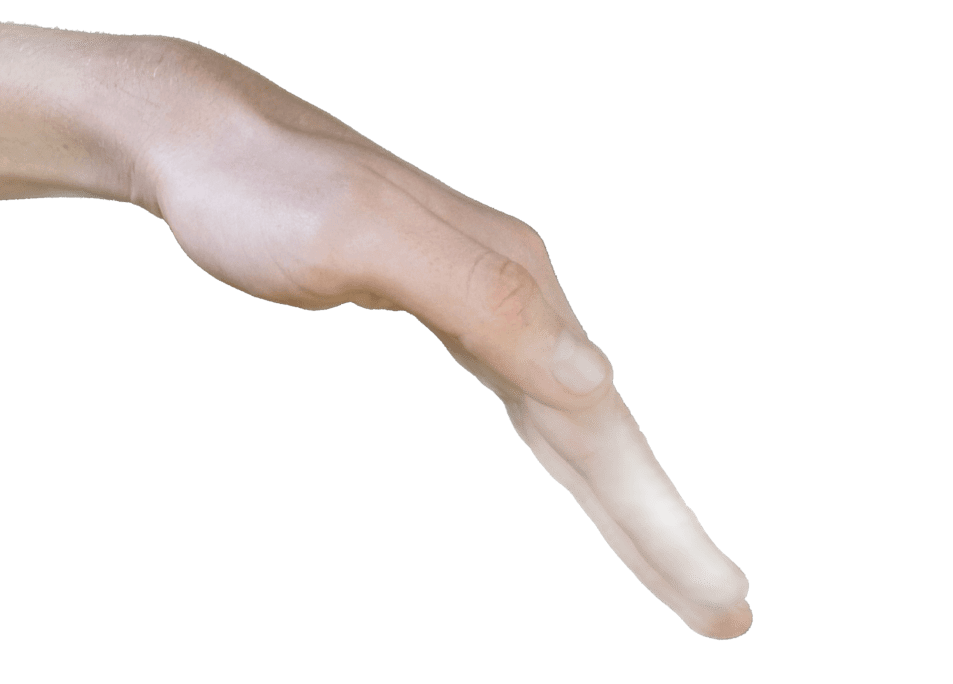
\includegraphics[width=\linewidth]{gesture_images/flexion_above.png} & 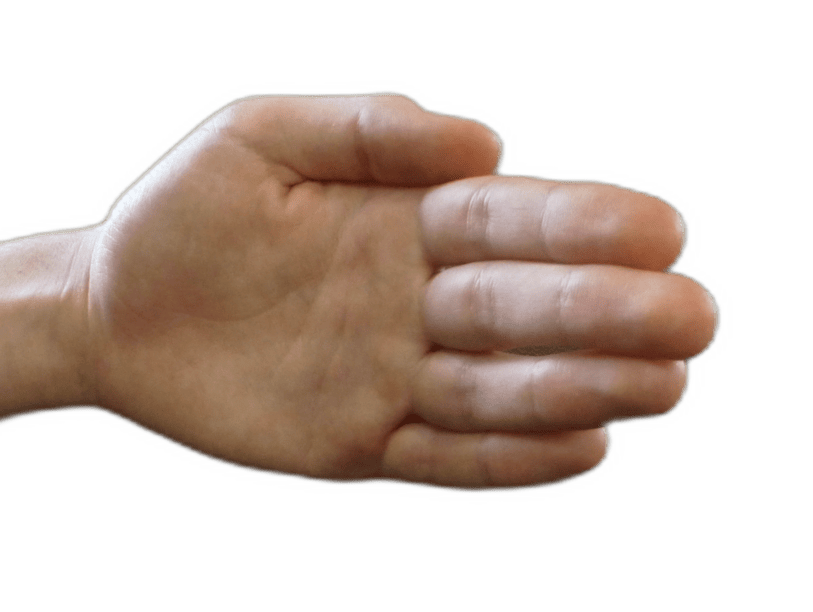
\includegraphics[width=\linewidth]{gesture_images/flexion_side.png} \\ \hline
            Adduction & 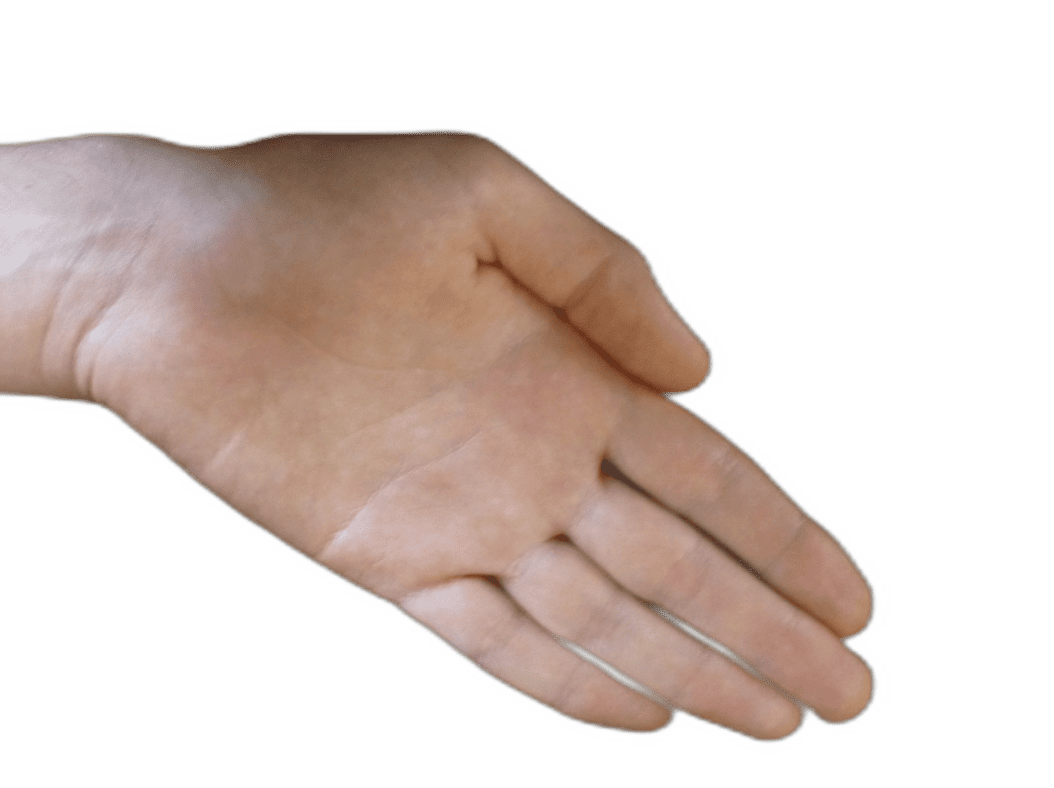
\includegraphics[width=\linewidth]{gesture_images/adduction_above.png} & 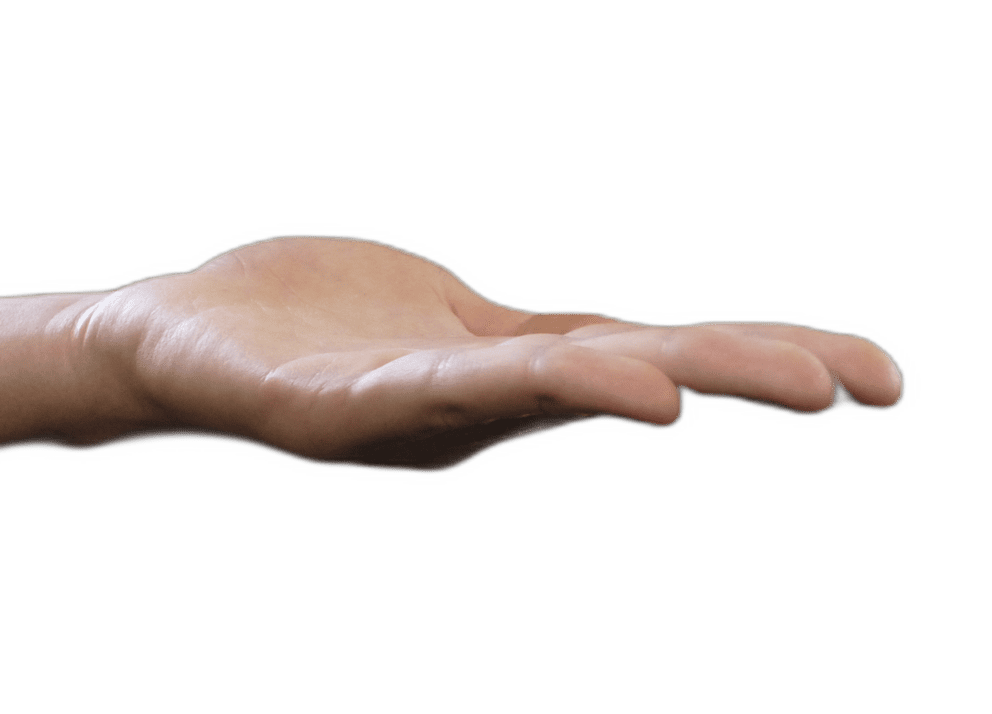
\includegraphics[width=\linewidth]{gesture_images/adduction_side.png} \\ \hline
        \end{tabular}
    \end{minipage}
    }
    \caption{Table 4.1: Gesture Table \cite{diamand2025}\cite{McIntosh2017SensIR:Reflection}\cite{Alexander2024HaGRIDDataset}}
    \label{tab:gesture_set_final}
\end{table}

\label{chap:evaluation}

\section{Experiment Design}
We collected data from 11 participants. Each participant completed two sessions, one for each type of LED. A session involved performing 20 trials of 20 gestures, with the order of gestures in each batch randomised, while wearing the FlexIR wristband. The order in which users completed the sessions was counterbalanced to avoid order effects such as fatigue.

In each session:

\begin{itemize}
    \item The wristband is placed on the user
    \item A gesture is shown on screen
    \item The user replicates the gesture and the study conductor verifies the gesture is correct
    \item A capture of the gesture is recorded
\end{itemize}

Each capture consists of 10 readings taken at 0.1 second intervals. The 10 sequential readings, referred to as captures, are kept together during outlier removal, data shuffling and splitting to prevent artificially increasing model performance.

\subsection{Software}

\autoref{fig:software} shows data collection software, adapted from Python code provided by GestIR \cite{diamand2025}. The data collection software used the USB port to send commands to the FlexIR wristband and receive sensor readings. Users were prompted with images of hand gestures, which they were asked to replicate before pressing a key to save the capture. The live sensor readings were also displayed, which allowed for easy debugging of wristband segments. When participants completed a session, the gesture data was saved to a JSON file.

The machine learning models were also adapted from code provided by GestIR \cite{diamand2025}. These consisted of MLPs and CNNs written using TensorFlow, and random forests written using scikit-learn.

\begin{figure}
    \centering
    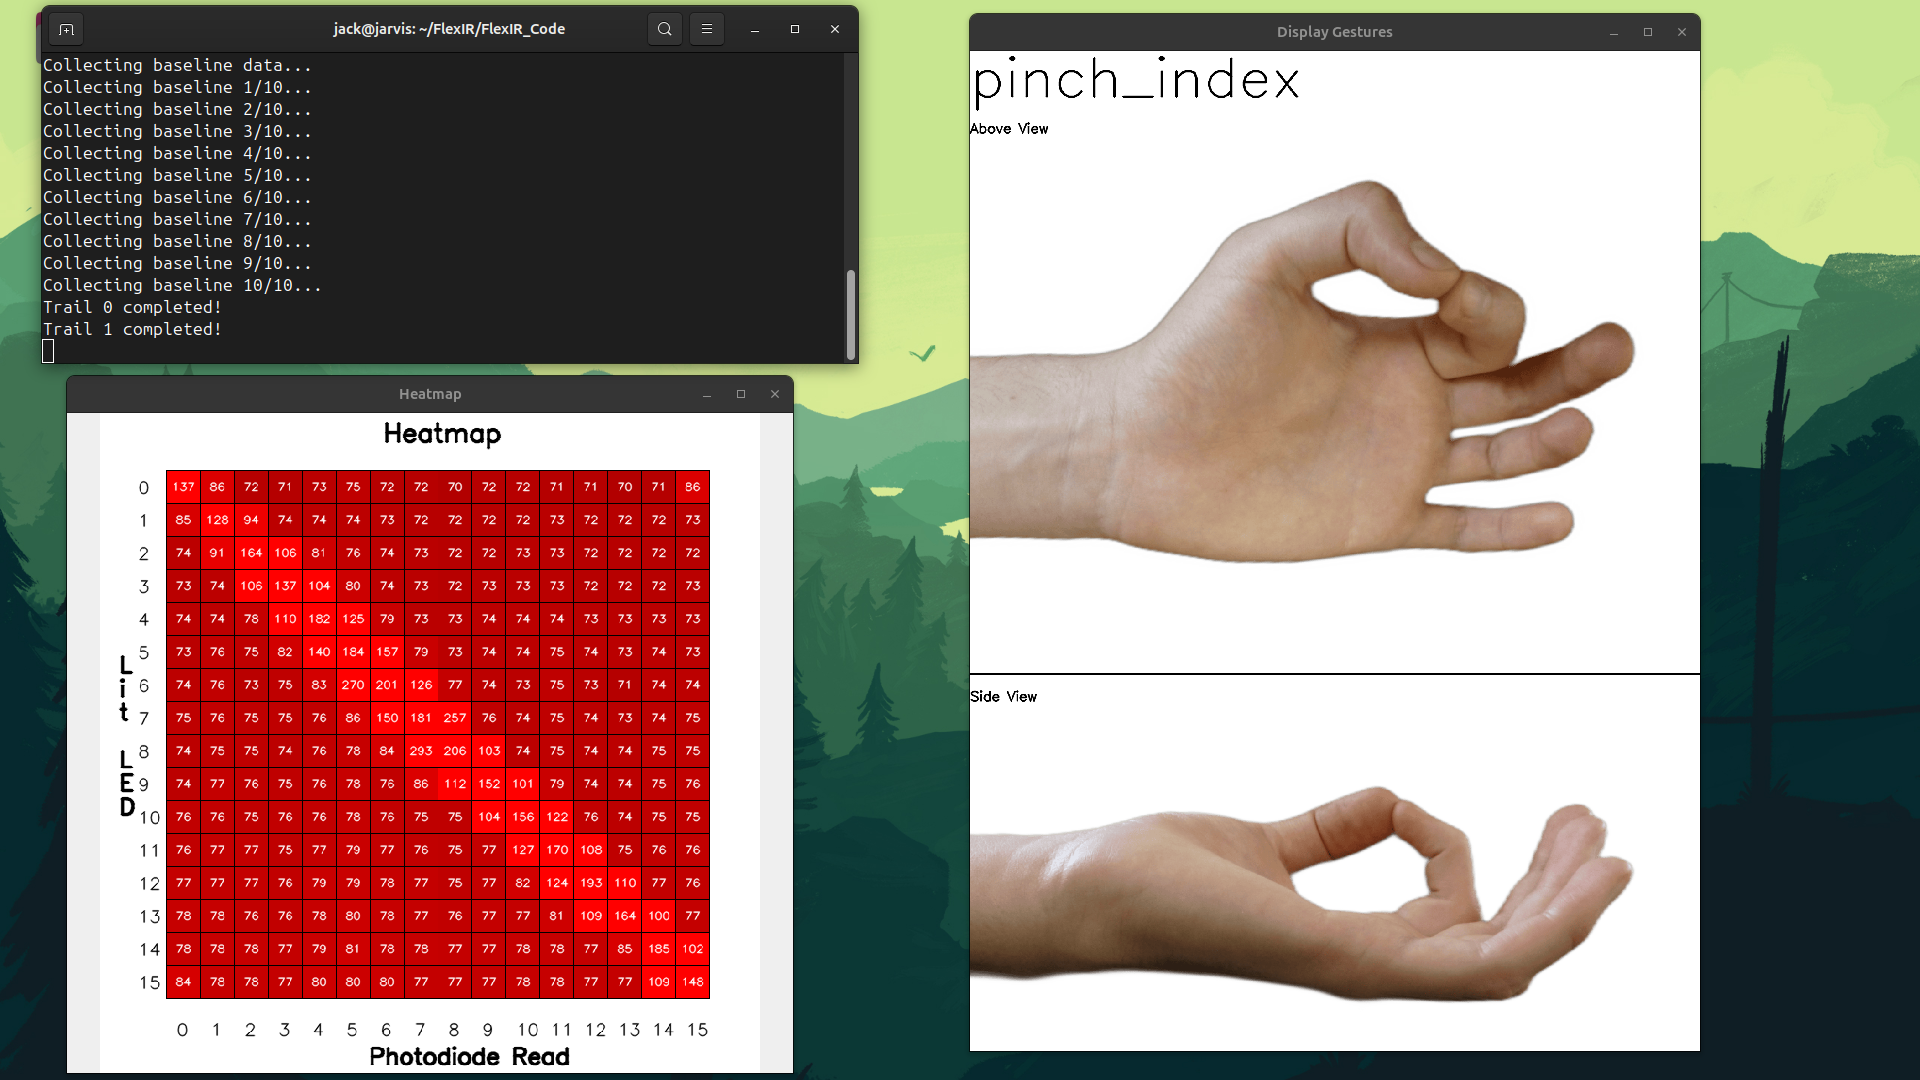
\includegraphics[width=1\linewidth]{software.png}
    \caption{Data collection software}
    \label{fig:software}
\end{figure}

\section{Machine Learning Models}
Like GestIR and SensIR, cross-user generalisation was not attempted due to anatomical differences between participants - separate models were trained for each participant. Also, since the data captured from FlexIR is very similar to GestIR, the GestIR machine learning models were used as starting points for this project.

\subsection{Model Selection}
The data captured from GestIR and FlexIR is structured, grid-like data. The captures are also toroidal in structure - the wristband is circular (the first and last segments are physical neighbours), so the top and bottom, and the left and right, of the matrix can be considered adjacent. 

Convolutional neural networks (CNNs) perform well on structured, grid like data such as images. Because of this, they were expected to be most effective for this application. GestIR evaluated standard CNNs, toroidal CNNs that match the toroidal structure of the captures, as well as standard MLPs.

Despite the toroidal CNNs more closely resembling the shape of the input data, the MLPs performed the best, achieving an average of 85.8\% test accuracy with 950nm LEDs\cite{diamand2025}. We briefly evaluated the standard and toroidal CNNs on FlexIR using the same parameters, and found similar results (\autoref{fig:all_model_accuracies}). This supports GestIRs findings that high model complexity isn't necessary for accurate gesture recognition.

\begin{figure}[htp]
    \centering
    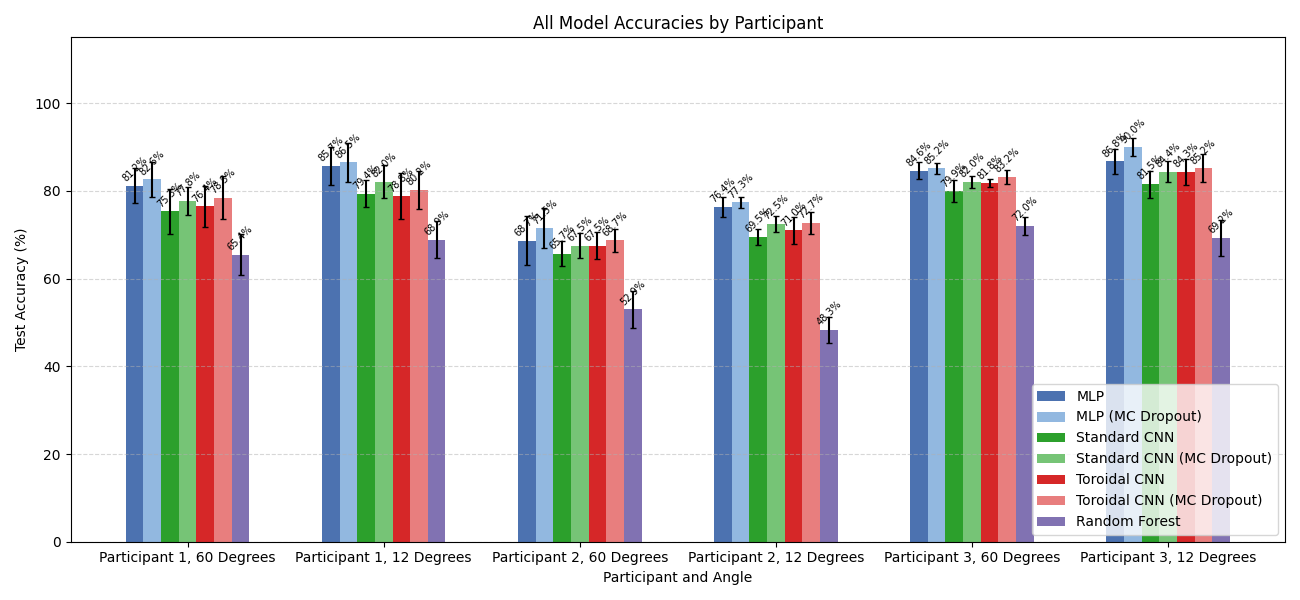
\includegraphics[width=\textwidth]{figures/accuracy_comparison_all.png}
    \caption{Accuracies of all models trained on initial wristband data for the first three participants}
    \label{fig:all_model_accuracies}
\end{figure}

In this project, a small but consistent performance boost was achieved by running the models described in GestIR in addition to Monte Carlo dropout.

To save time, only the best performing models were trained on final experiment data. The final model architecture was an MLP with the same pyramidal architecture as GestIR ($512 \rightarrow 256 \rightarrow 128 \rightarrow 128 \rightarrow 64$), in addition to 50 iterations of Monte Carlo dropout. This architecture is likely oversized for the application, and training and inference were run on a laptop rather than the microcontroller. Model optimisation wasn't the aim of this project, and future research into the effectiveness of models with fewer parameters is necessary to determine the feasibility of classification on-board the microcontroller.

\subsection{Hardware Faults}
Part way through data collection, the photodiodes on two segments of the $\pm 12^\circ$ wristband developed a fault. Due to time constraints, it wasn't feasible to manufacture a new wristband. \autoref{fig:heatmap_faulty} shows an example of a 16x16 reading recorded with the faulty wristband. Data recorded on those two photodiodes were removed from all participants datasets, resulting in 16x14 capture matrices.

\begin{figure}[htp]
    \centering
    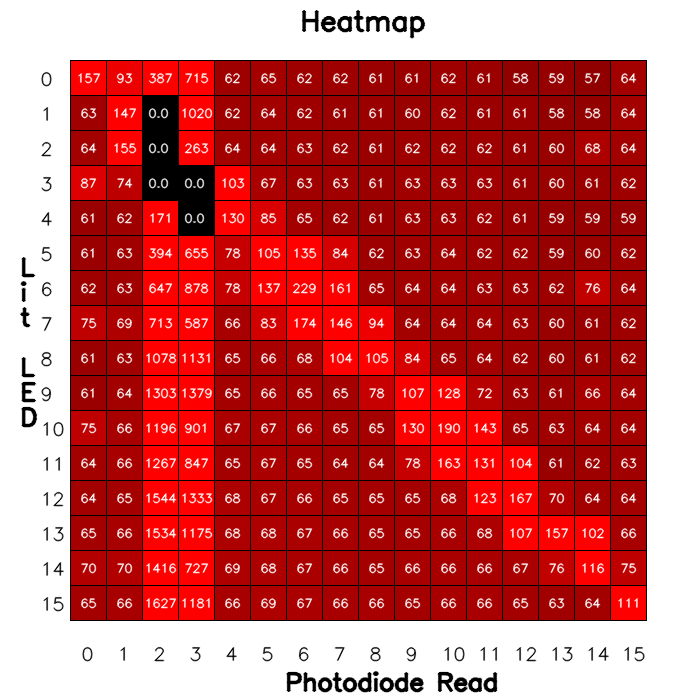
\includegraphics[width=0.35\textwidth]{figures/heatmap_faulty.png}
    \caption{A heatmap showing the faulty photodiodes in segments 2 and 3}
    \label{fig:heatmap_faulty}
\end{figure}

\section{Findings}
This section details the performance of the the models trained to classify the hand gestures. To investigate how informative data for gesture recognition is generated, we created a range of datasets consisting of specific features. \autoref{sec:all_features} analyses the overall model accuracies, comparing the performance of both wristbands, identifying the most commonly misclassified gestures, and investigating how much training data the models need to learn gestures. \autoref{sec:reflection_transmission} restricts the dataset to features designed to isolate data generated by deep tissue interactions from data generated by superficial reflections. \autoref{sec:smartwatch} explores the possibility of future integration into smartwatch devices by analysing accuracies of models trained on sensor data from the dorsal side of the wrist only.
% \autoref{sec:all_features} analyses the overall model accuracies, comparing the accuracies of the wristbands and identifying the most commonly misclassified gestures. \autoref{sec:reflection_transmission} contains accuracies for models trained only on specific features of the data. \autoref{sec:smartwatch} contains accuracies for models trained on sensor data from the dorsal side of the wrist only, exploring the possibility of future integration into smartwatch devices. For all these experiments, paired $t$-tests were conducted to compare the accuracies of the $\pm 12^\circ$ and $\pm 60^\circ$ wristbands. \autoref{sec:confounding_variables} conducts statistical tests to check for order effects and environmental effects. \autoref{sec:wrist_circumference} shows correlation between the gesture recognition accuracy across all experiments and the participants' wrist circumferences.

For all the statistical tests, a significance level of $\alpha=0.05$ was used. The tests are split into seven families:
\begin{itemize}
    \item Paired $t$-tests comparing the accuracies of the $\pm 12^\circ$ and $\pm 60^\circ$ wristbands when trained using different sets of features
    \item Paired $t$-tests comparing the accuracies of the $\pm 12^\circ$ and $\pm 60^\circ$ when trained on varying training set sizes
    \item Paired $t$-tests comparing the performance of models trained on different features to the performance of models trained on all features (including an investigation into the performance drop when removing photodiodes 2 and 3 from the dataset)
    \item Unpaired $t$-tests investigating order effects
    \item Permutation tests investigating environmental effects
    \item Pearson correlation tests between model performance and participant wrist circumference
    \item Paired $t$-tests comparing the accuracies of models trained on the full gesture set vs the gesture set excluding pinch gestures
    
\end{itemize}
Although the data for these tests all were produced from the same user trials, the seven families represent distinct hypotheses. For each of these families, the $p$-values were corrected for multiple comparisons using the Benjamini-Hochberg procedure. $p_{adj}$ refers to the FDR adjusted $p$-values. 

\subsection{All Features}
\label{sec:all_features}
\label{sub}
\begin{figure}[htp]     
    \centering
     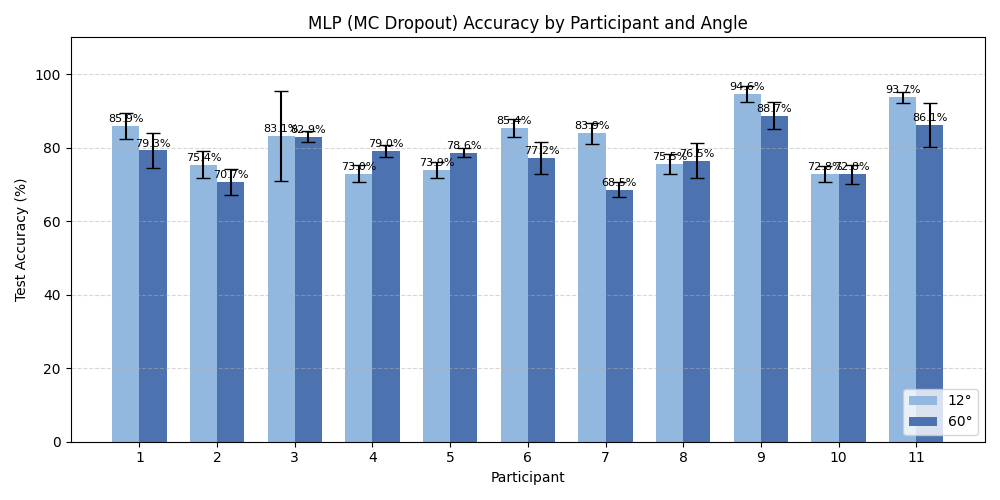
\includegraphics[width=0.9\textwidth]{figures/accuracy_mlp_mc_dropout_by_angle.png}
     \caption{Classification accuracy for all participants and both wristbands (MLPs with Monte Carlo dropout trained on all features)}
     \label{fig:accuracy_all}
\end{figure}

\subsubsection{Overall Model Accuracy}
\autoref{fig:accuracy_all} shows the average accuracy of MLPs with Monte Carlo dropout trained on data from the $\pm 12^\circ$ and $\pm 60^\circ$ wristbands across all participants. To account for variation introduced by data partitioning, we trained five models on different stratified splits of the data. The bars show the mean model performance, with error bars representing the standard deviation. 

Overall, the $\pm 12^\circ$ wristband performed marginally better, averaging 81.6\% accuracy compared to 78.2\% accuracy with the $\pm 60^\circ$ wristband. However, the results were noisy, varying between participants. 

A paired $t$-test was conducted to compare the average model performance between the two wristbands. Overall, there was no statistical significance between the two wristbands ($t$ = 1.758, $p$ = 0.109, $p_{adj}$ = 0.124, Cohen's $d$ = -0.530).

\subsubsection{Performance Reduction Due To Missing Segments}

\begin{figure}[htp]
     \centering
     \begin{subfigure}[b]{0.48\textwidth}
         \centering
         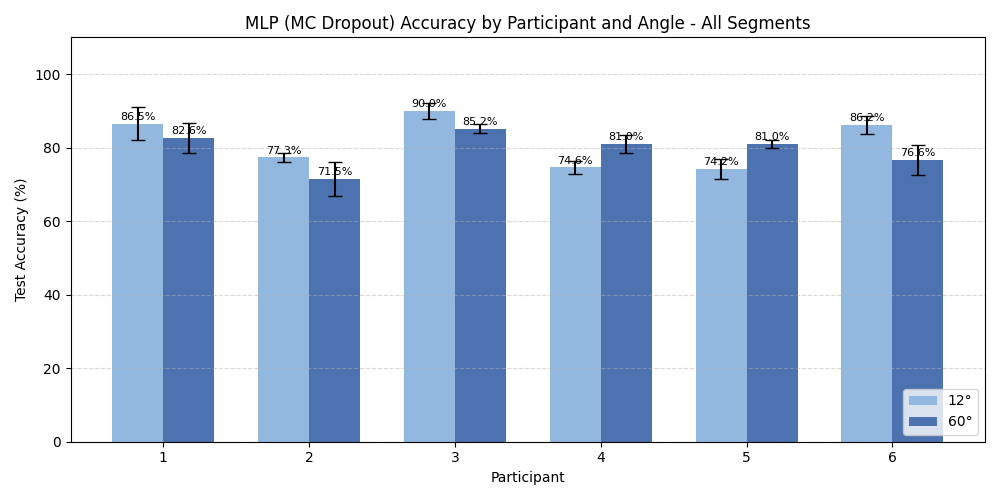
\includegraphics[width=\textwidth]{figures/accuracy_mlp_mc_dropout_by_angle_p1-6_all_features.png}
         \caption{All segments}
         \label{fig:accuracy_all_segments}
     \end{subfigure}
      \begin{subfigure}[b]{0.48\textwidth}
         \centering
         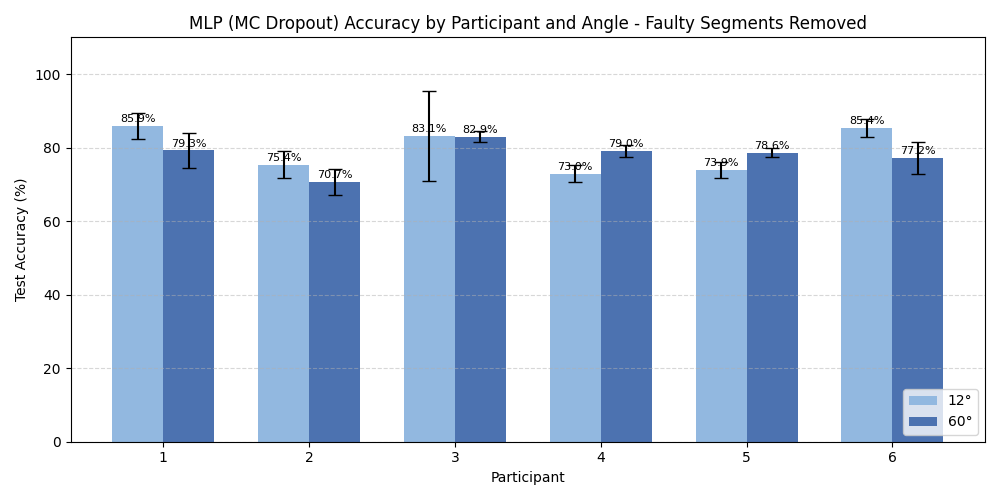
\includegraphics[width=\textwidth]{figures/accuracy_mlp_mc_dropout_by_angle_p1-6.png}
         \caption{Broken segments removed}
         \label{fig:accuracy_broken_segments}
     \end{subfigure}
    \caption{Accuracy of models trained on all segment data (\autoref{fig:accuracy_all_segments}) and data with faulty segments removed (\autoref{fig:accuracy_broken_segments})}
    \label{fig:broken_segments_graph}
\end{figure}

A fault developed with two segments of the wristband halfway through data collection. Because of this, data collected from photodiodes 2 and 3 is removed from all participants, resulting in 16x14 readings.

\autoref{fig:broken_segments_graph} shows the accuracies of initial models trained on the full 16x16 readings compared to the accuracies of models trained on the same participants but with photodiodes 2 and 3 removed.

For the $\pm 60^\circ$ wristband, a paired $t$-test between the accuracies of the models before and after removing the segments revealed that the performance drop was significant ($t$ = 2.966, $p$ = 0.031, $p_{adj}$ = 0.045, Cohen's $d$ = -1.211). The average performance decrease was 1.69\%.

For the $\pm 12^\circ$ wristband, the accuracy drop was not statistically significant. However, the huge increase in standard deviation for the models trained on participant 3 (shown by the error bars in \autoref{fig:broken_segments_graph}) shows that removing the segments produced less robust models.

Therefore, on a fully functioning wristband, we would expect a small performance boost of 1.69\% on the $\pm 60^\circ$ wristband, which would result in an overall accuracy of 79.9\%. We would also expect more robust and reliable models with lower variance in accuracies.

\subsubsection{Confusion Matrices}

The confusion matrices in \autoref{fig:cf_all} show the predicted and true labels for gestures in the test set. Like SensIR \cite{McIntosh2017SensIR:Reflection} and GestIR \cite{diamand2025}, the most confusion came from the four pinch gestures (pinch\_index, pinch\_middle, pinch\_ring, pinch\_pinkie). These accounted for 43.1\% of misclassifications on the $\pm 12^\circ$ wristband and 41.9\% of the misclassifications on the $\pm 60^\circ$ wristband. This suggests that gestures involving precise finger movement with similar overall hand positions are difficult for IR systems to detect.

Models trained on data excluding the pinch gestures achieved average accuracies of 89.0\% and 86.7\% on the $\pm 12^\circ$ and $\pm 60^\circ$ respectively. Paired $t$-tests found the performance increase compared to models trained to classify the full gesture set to be statistically significant ($t$ = -5.992, $p <$ 0.001, $p_{adj} <$ 0.001, Cohen's $d$ = 1.807 for the $\pm 12^\circ$ wristband and $t$ = -8.938, $p <$ 0.001, $p_{adj} <$ 0.001, Cohen's $d$ = 2.695 for the $\pm 60^\circ$ wristband).

\begin{figure}[h]     
    \centering
     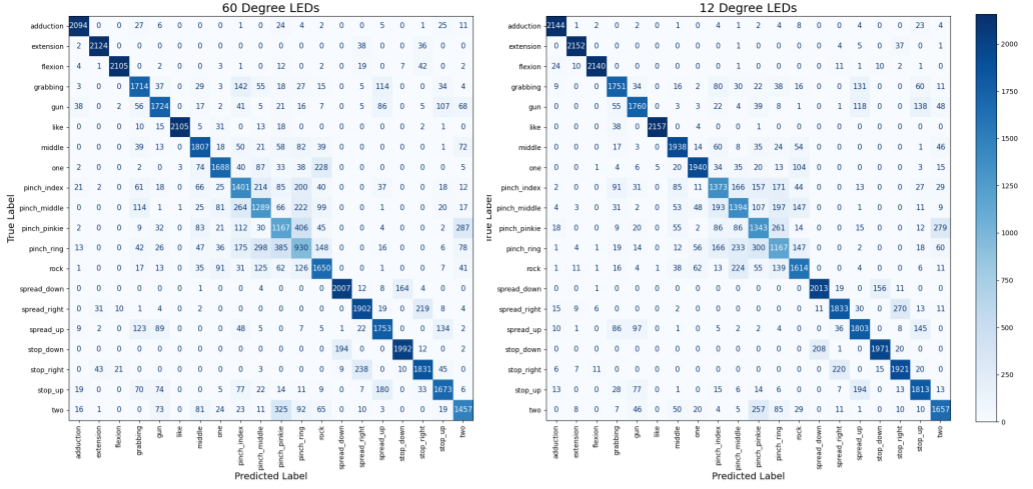
\includegraphics[width=\textwidth]{figures/CF_all.png}
     \caption{Confusion matrices for MLPs with Monte Carlo dropout trained on all features, aggregated over all participants}
     \label{fig:cf_all}
\end{figure}

\subsubsection{Number of Training Samples}
Twenty trials of data collection were selected as a balance between collecting sufficient data for robust results and maintaining user comfort. However, participants still reported some fatigue and discomfort during long data collection sessions. To inform future experiment design, we investigated the effect of reducing the number of trials on model performance.

The total datasets for each participant contain 20 trials of 20 gestures, resulting in 400 captures. The test, train validation split of 70\%, 10\% and 10\% produces a training set size of 280 captures. To evaluate the impact of reducing the dataset size, we trained models using stratified subsamples of the test set. Models were trained on training sets of size 70, 140, 210, and 280 captures, with fixed validation and test sets. This was repeated for five test/train/validation splits.

\begin{figure}[htp]
     \centering
     \begin{subfigure}[b]{0.4\textwidth}
         \centering
         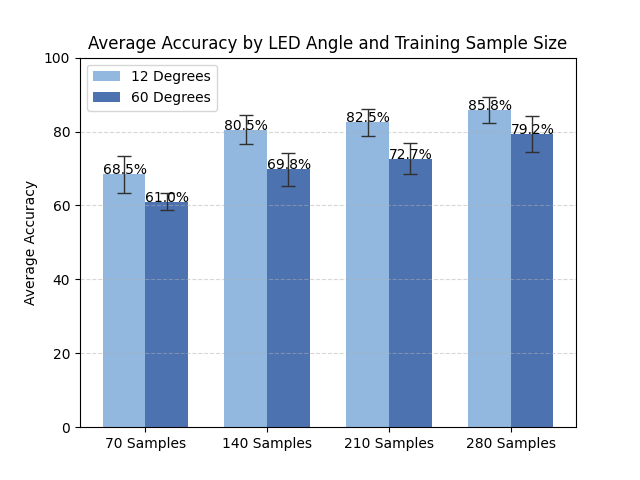
\includegraphics[width=\textwidth]{figures/sample_size_comparison_1.png}
         \caption{Participant 1}
         \label{fig:samples_participant_1}
     \end{subfigure}
      \begin{subfigure}[b]{0.4\textwidth}
         \centering
         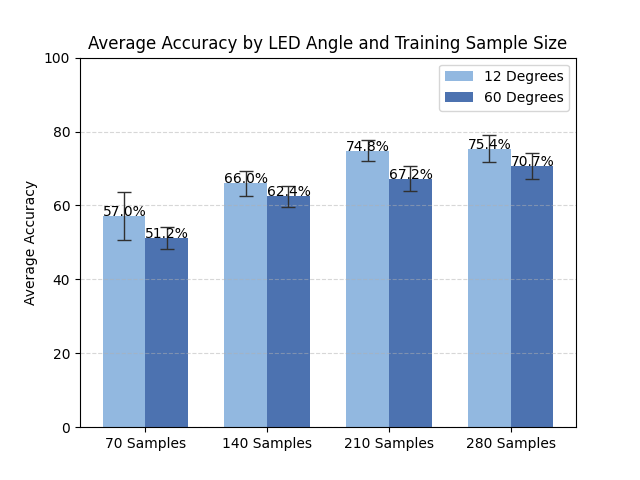
\includegraphics[width=\textwidth]{figures/sample_size_comparison_2.png}
         \caption{Participant 2}
         \label{fig:samples_participant_2}
     \end{subfigure}
      \begin{subfigure}[b]{0.4\textwidth}
         \centering
         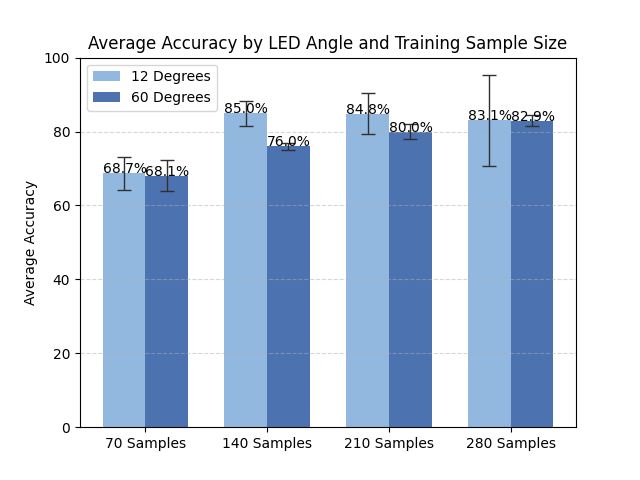
\includegraphics[width=\textwidth]{figures/sample_size_comparison_3.png}
         \caption{Participant 3}
         \label{fig:samples_participant_3}
     \end{subfigure}
    \caption{Average model accuracy vs size of training set}
    \label{fig:samples_test}
\end{figure}

\autoref{fig:samples_test} shows the average model accuracies for participants 1, 2, and 3 for each subsample of training data, with error bars representing the standard deviation. Graphs for all participants can be found in \autoref{appx:samples}. The graphs vary between participants, but in general, the performance increases as the number of training captures increases. The accuracy begins to plateau with the full 280 captures. However, the large error bars show that model performance is highly dependent on specific data splitting. More training data would likely reduce this sensitivity to specific portions of the data and produce more robust models.

We conducted paired $t$-tests to compare the accuracies of the $\pm 12^\circ$ and $\pm 60^\circ$ wristbands for these models. This revealed no significant difference between the performance of the wristbands for any of the subsamples of training data, showing no evidence that the LED viewing angle is a factor in how much training data the models need to learn gestures.
     
\subsection{Reflection and Transmission Features}
\label{sec:reflection_transmission}

The most informative data for gesture recognition is produced by light that's reflected off/near the surface of the skin. This means readings from photodiodes close to the currently active LED provide the  most useful data. The bright diagonal band on the capture matrices show the more intense readings from photodiodes that correspond to the active LED.

We define \textbf{reflection features} as readings from photodiodes that are close in physical proximity to the currently active LED. \textbf{Transmission features }are readings from photodiodes far away from the currently active LED. In this section, we analyse the performance of models when trained on data only containing reflection or transmission features. The \textbf{band width} of a reading containing only reflection or transmission features is the number of photodiodes preserved or ignored.

\begin{figure}[htp]
     \centering
     \begin{subfigure}[b]{0.3\textwidth}
         \centering
         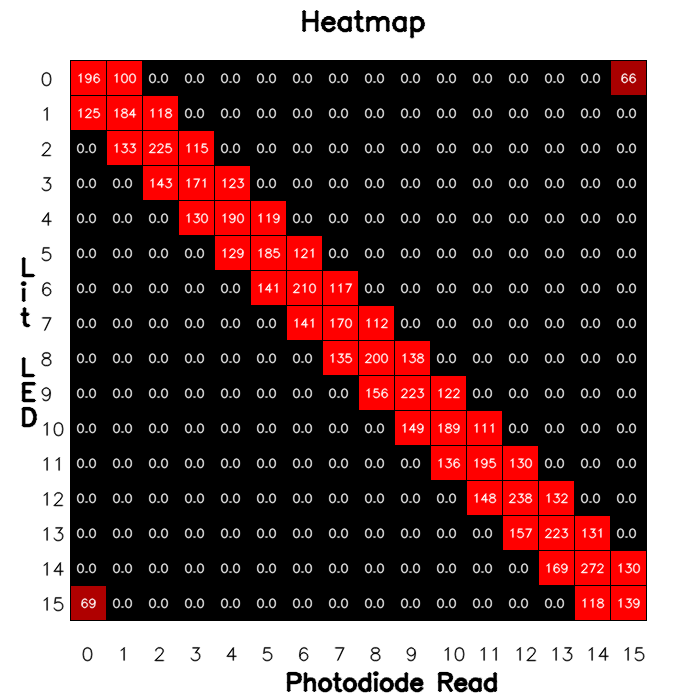
\includegraphics[width=\textwidth]{figures/heatmap_reflection_3.png}
         \caption{Reflection features, band width 3}
         \label{fig:heatmap_reflection_3}
     \end{subfigure}
      \begin{subfigure}[b]{0.3\textwidth}
         \centering
         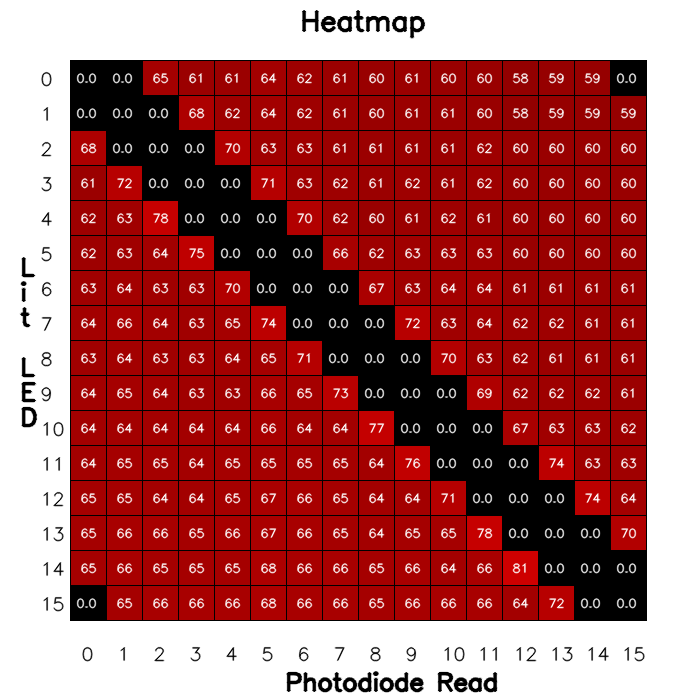
\includegraphics[width=\textwidth]{figures/heatmap_transmission_3.png}
         \caption{Transmission features, band width 3}
         \label{fig:heatmap_transmission_3}
     \end{subfigure}
     \begin{subfigure}[b]{0.3\textwidth}
         \centering
         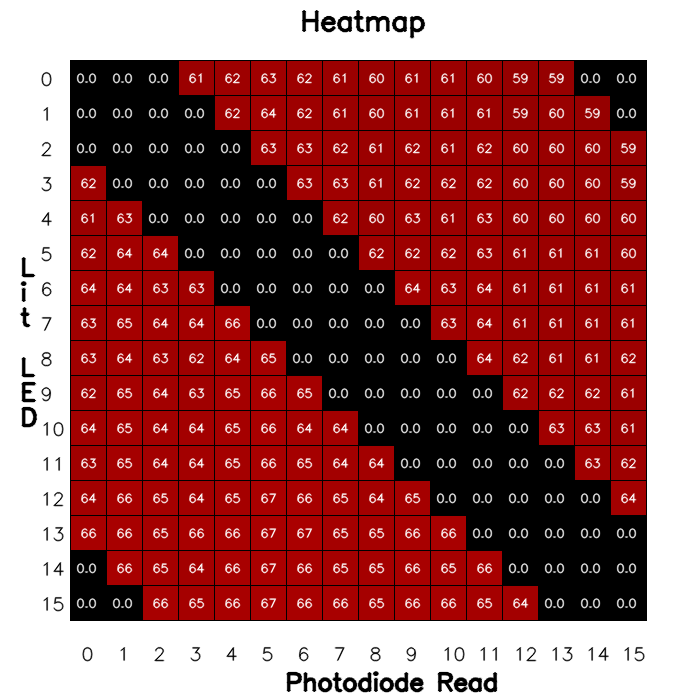
\includegraphics[width=\textwidth]{figures/heatmap_transmission_5.png}
         \caption{Transmission features, band width 5}
         \label{fig:heatmap_transmission_5}
     \end{subfigure}
    \caption{Heatmaps showing readings with all features included, transmission features with a diagonal band of width 3 removed, and transmission features with a diagonal band of width 5 removed}
    \label{fig:heatmmaps}
\end{figure}

To generate data containing only reflection or transmission features, we set the relevant parts of the capture matrix to zero. \autoref{fig:heatmmaps} shows readings containing reflection and transmission features with band width 3 and transmission features with band width 5.

\subsubsection{Reflection Features}
We trained models using data with only reflection features with a band width of 3. A paired $t$-test between these accuracies and the accuracies of models trained on all data wasn't significant for either wristband. This indicates that reflection features generated from photodiodes physically close to the active LEDs provide sufficient information and that transmission features may not be necessary for gesture recognition.

\subsubsection{Transmission Features}

When training on transmission features only, the overall accuracy drops significantly compared to models trained on all features. However, the accuracy of the $\pm 12^\circ$ LED wristband is much higher than the $\pm 60^\circ$ wristband.

\begin{figure}[htp]     
    \centering
     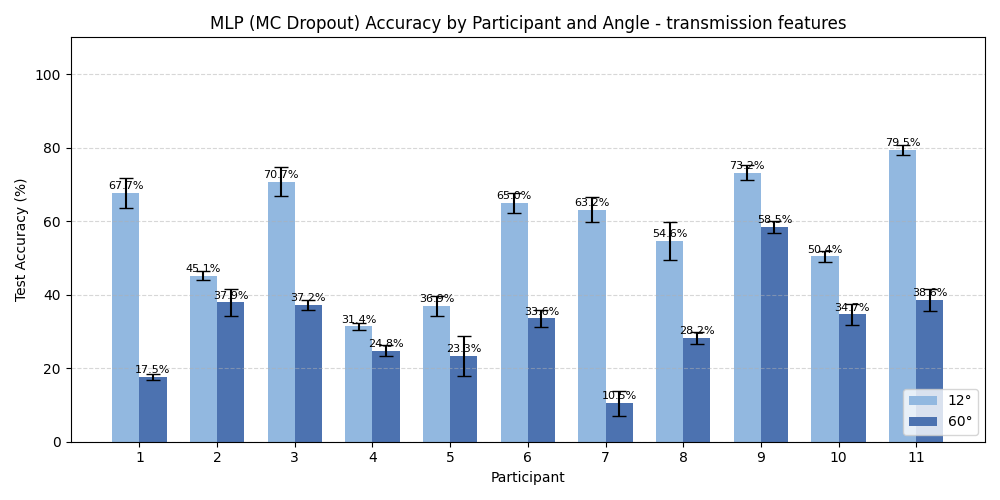
\includegraphics[width=0.9\textwidth]{figures/accuracy_mlp_mc_dropout_by_angle_transmission.png}
     \caption{MLP with Monte Carlo dropout classification accuracy for all participants and both wristbands, trained on transmission with band width 3}
     \label{fig:accuracy_transmission_3}
\end{figure}

\autoref{fig:accuracy_transmission_3} shows  the average accuracy of MLPs with Monte Carlo dropout trained on data for both wristbands, using only transmission features with a diagonal band of width 3 removed from the captures. The $\pm 12^\circ$ wristband achieves an average accuracy of 58.0\%, and the $\pm 60^\circ$ wristband achieves 31.4\%. Paired $t$-tests between these accuracies and the accuracies of models trained on all features were statistically significant ($t$ = 8.609, $p <$ 0.001, $p_{adj} <$ 0.001, Cohen's $d$ = -2.596 for the $\pm 12^\circ$ wristband and $t$ = 15.284, $p <$ 0.001, $p_{adj} <$ 0.001, Cohen's $d$ = -4.608 for the $\pm 60^\circ$ wristband), showing a clear drop in performance.

We conducted a paired $t$-test to compare the average accuracies of each wristband. This showed a significant difference ($t$ = 5.362, $p <$ 0.001, $p_{adj}$ = 0.002, Cohen's $d$ = -1.617), indicating that when restricted to transmission features, $\pm 12^\circ$ LEDs outperform $\pm 60^\circ$ LEDs.

\begin{figure}[htp]     
    \centering
     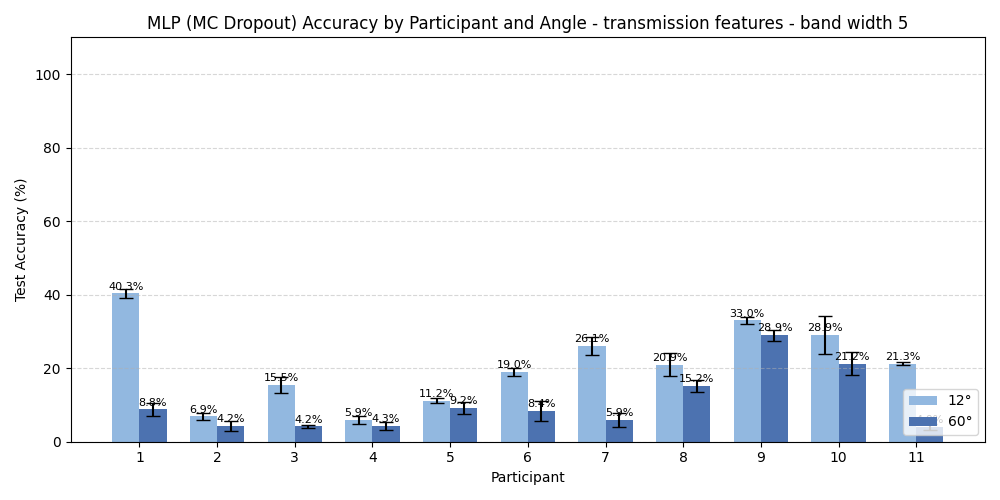
\includegraphics[width=0.9\textwidth]{figures/accuracy_mlp_mc_dropout_by_angle_transmission_band5.png}
     \caption{MLP with Monte Carlo dropout classification accuracy for all participants and both wristbands, trained on transmission features with band width 5}
     \label{fig:accuracy_transmission_5}
\end{figure}

\autoref{fig:accuracy_transmission_5} shows the average accuracy of models trained on transmission features with a band width of 5. The average accuracy of the $\pm 12^\circ$ is 20.8\%, and the average accuracy of the $\pm 60^\circ$ wristband is 10.4\%. Again, the accuracy of both wristbands was lower than when training with all features ($t$ = 21.445, $p <$ 0.001, $p_{adj} <$ 0.001, Cohen's $d$ = -6.467 for the $\pm 12^\circ$ wristband and $t$ = 25.373, $p <$ 0.001, $p_{adj} <$ 0.001, Cohen's $d$ = -7.650).

A paired $t$-test also revealed the accuracy of the $\pm 12^\circ$ wristband was significantly higher ($t$ = 3.709, $p$ = 0.004, $p_{adj}$ = 0.012, Cohen's $d$ = -1.118). 

\subsection{Smartwatch Features}
\label{sec:smartwatch}
Many smartwatches already make use of optical sensing to measure heart rate. A gesture recognition device that only uses sensors on the dorsal side of the wrist would offer more practical integration with the main body of existing smartwatch designs, without the need for sensors in the strap surrounding the wrist. To evaluate the potential of this, we trained models on data produced by four segments spanning 36 mm across the dorsal side of the wrist.

\begin{figure}[htp]     
    \centering
     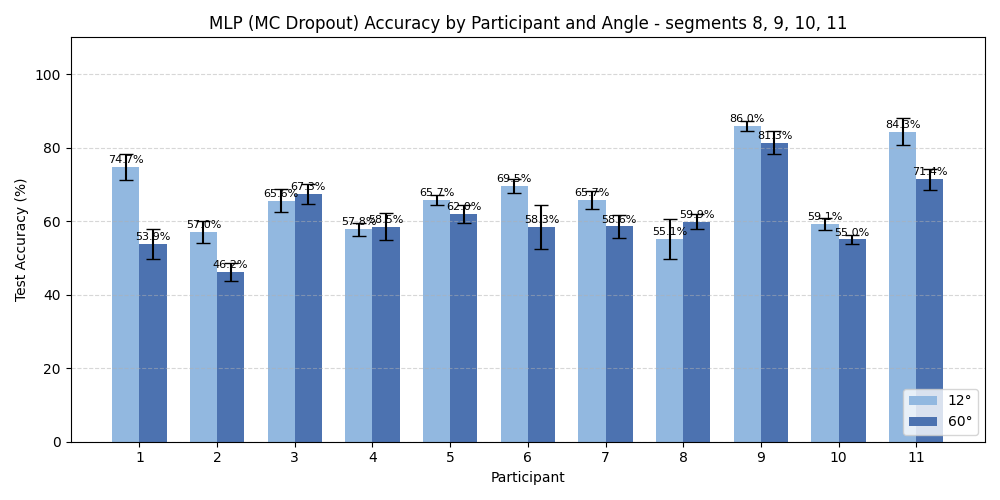
\includegraphics[width=0.9\textwidth]{figures/accuracy_mlp_mc_dropout_by_angle_segments_8-9-10-11.png}
     \caption{MLP with Monte Carlo dropout classification accuracy for all participants and both wristbands, trained on segments 8, 9, 10, and 11 only}
     \label{fig:accuracy_smartwatch}
\end{figure}

\autoref{fig:accuracy_smartwatch} shows the average accuracy of models trained using only data from photodiodes 8, 9, 10, and 11. The $\pm 12^\circ$ wristband had an average accuracy of 67.3\% and the $\pm 60^\circ$ wristband had an average accuracy of 61.1\%. The performance drop of 14.3\% and 17.1\% when compared to models trained on all segments were statistically significant ($t$ = 10.937, $p <$ 0.001, $p_{adj} <$ 0.001, Cohen's $d$ = -3.298 for the $\pm 12^\circ$ wristband and $p$ = 10.474, $p <$ 0.001, $p_{adj} <$ 0.001, Cohen's $d$ = -3.158 for the $\pm 60^\circ$ wristband). A paired $t$-test between the accuracies for both wristbands revealed that the $\pm 12^\circ$ wristband performs significantly better on smartwatch features ($t$ = 2.773, $p$ = 0.020, $p_{adj}$ = 0.039, Cohen's $d$ = -0.836). 

\subsection{Correlation With Wrist Circumference}
\label{sec:wrist_circumference}
Model performance varies between participants, most likely because of anatomical differences between the wrists. One hypothesis was that wrist circumference was a factor in how well the wristbands performed, due to the assumption that thicker wrists are less transmissive to IR light and produce less informative transmission features. To investigate this, we compared the model accuracies with the participants wrist circumferences.

\begin{figure}[htp]     
    \centering
     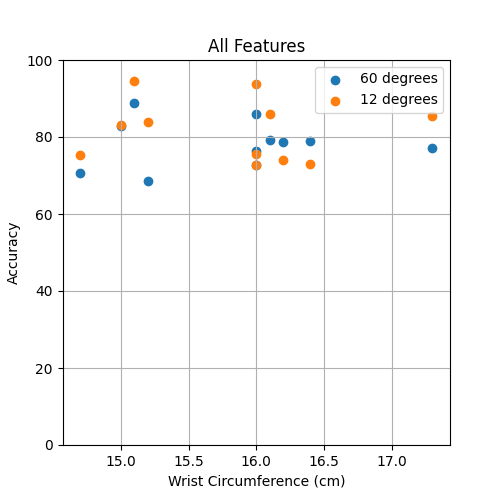
\includegraphics[width=0.6\textwidth]{figures/accuracy_vs_wrist_size_all.png}
     \caption{Scatter plot showing the average model accuracy trained on all features vs wrist circumference for all participants.}
     \label{fig:accuracy_vs_circumference}
\end{figure}

Wrist circumference was measured 1.5 cm from the centre of the ulnar styloid (the same place the wristbands were worn during data collection) with the fist clenched. \autoref{fig:accuracy_vs_circumference} shows scatter plots comparing model accuracies with wrist circumferences for models trained on all features. After FDR adjustment, the results were all insignificant, showing there is no evidence of a linear relationship between wrist circumference and wristband performance. Scatter plots for all experiments can be found in \autoref{appx:acc_vs_wrist_size}. 

% Wrist circumference was measured 1.5 cm from the centre of the ulnar styloid (the same place the wristbands were worn during data collection) with the fist clenched. \autoref{fig:accuracy_vs_circumference} shows scatter plots comparing model accuracies with wrist circumferences for models trained on all features. \autoref{tab:correlation_results_12} and \autoref{tab:correlation_results_60} show the results of Pearson correlation tests on the $\pm 12^\circ$ and $\pm 60^\circ$ wristbands. The adjusted $p$-values are all insignificant, showing there is no evidence of a linear relationship between wrist circumference and wristband performance. Scatter plots for all experiments can be found in \autoref{appx:acc_vs_wrist_size}.

% \begin{table}[htp]
%     \centering
%     \begin{tabular}{lrrr}
%         \toprule
%         Experiment & $r$ & $p$ & $p_{adj}$ \\
%         \midrule
%         All Features, All Gestures & -0.112 & 0.743 & 0.999 \\
%         All Features, Excluding Pinch Gestures & -0.007 & 0.983 & 0.999 \\
%         Transmission Features (Band Width 3), All Gestures & -0.160 & 0.638 & 0.999 \\
%         Transmission Features (Band Width 5), All Gestures & 0.000 & 0.999 & 0.999 \\
%         Reflection Features (Band Width 3), All Gestures & -0.193 & 0.569 & 0.999 \\
%         Smartwatch Features, All Gestures & -0.011 & 0.975 & 0.999 \\
%         \bottomrule
%     \end{tabular}
%     \caption{Results of the Pearson correlation tests between the model accuracies and wrist circumferences for the $\pm 12\circ$ wristband}
%     \label{tab:correlation_results_12}
% \end{table}

% \begin{table}[htp]
%     \centering
%     \begin{tabular}{lrrr}
%         \toprule
%         Experiment & $r$ & $p$ & $p_{adj}$ \\
%         \midrule
%         All Features, All Gestures & 0.056 & 0.869 & 0.999 \\
%         All Features, Excluding Pinch Gestures & 0.141 & 0.679 & 0.999 \\
%         Transmission Features (Band Width 3), All Gestures & -0.259 & 0.442 & 0.999 \\
%         Transmission Features (Band Width 5), All Gestures & -0.069 & 0.840 & 0.999 \\
%         Reflection Features (Band Width 3), All Gestures & 0.089 & 0.794 & 0.999 \\
%         Smartwatch Features, All Gestures & -0.114 & 0.738 & 0.999 \\
%         \bottomrule
%     \end{tabular}
%     \caption{Results of the Pearson correlation tests between the model accuracies and wrist circumferences for the $\pm 60\circ$ wristband}
%     \label{tab:correlation_results_60}
% \end{table}

\subsection{Confounding Variables}
\label{sec:confounding_variables}
\subsubsection{Order Effects}
The order participants completed the data collection sessions was counterbalanced - group A used the $\pm 60^\circ$ wristband first, and group B used the $\pm 12^\circ$ first. To check for order effects, we calculated the difference in performance between the wristbands for each participant and performed Welch's unpaired $t$-tests on the performance differences of groups A and B. After FDR adjustment, the results were insignificant for all experiments, showing that there is no evidence that the order in which participants completed the sessions affected which wristband performed the best.


\subsubsection{Data Collection Locations}
Due to time constraints, data collection was conducted in three separate locations. Participants 1, 2, 3, 4, 5, 6 and 11 collected data in location A, participants 7 and 8 collected data in location B and participants 9 and 10 collected data in location C. In all locations, data collection was performed in a dark curtained room to minimise the impact of interference from background IR light.

Permutation tests were used to investigate any environmental effects. Permutation tests were chosen since they are more robust for the small sample sizes of locations B and C than other methods, e.g., Kruskal Wallis tests and ANOVA tests.

After FDR adjustment, the results of the permutation tests were insignificant for all experiments on both wristbands. This shows there was no evidence of any environmental effects on wristband performance.

\subsection{Summary of Results}
\autoref{tab:acc_summary} shows a summary of the classification accuracies of models trained on wristband data. \autoref{tab:results_summary} shows a summary of the significance of all the statistical tests conducted in \autoref{chapter:experiment}.

\begin{table}[htp]
    \centering
    \begin{tabular}{lrr}
        \toprule
        Experiment & $\pm 12^\circ$ LED Accuracy & $\pm 60^\circ$ LED Accuracy \\
        \midrule
        All Features, All Gestures & 81.6\% & 78.2\% \\
        All Features, Excluding Pinch Gestures & 89.0\% & 86.7\% \\
        Transmission Features (Band Width 3), All Gestures & 58.0\% & 31.4\% \\
        Transmission Features (Band Width 5), All Gestures & 20.8\% & 10.4\% \\
        Smartwatch Features, All Gestures & 67.3\% & 61.1\% \\
        \bottomrule
    \end{tabular}
    \caption{Summary of the classification accuracies for both LED viewing angles}
    \label{tab:acc_summary}
\end{table}

\begin{table}[htp]
    \centering
    \small
    \renewcommand{\arraystretch}{1.5} 
    \begin{tabularx}{\textwidth}{
        |>{\raggedright\arraybackslash}X|
        >{\raggedright\arraybackslash}X|
        >{\raggedright\arraybackslash}X|
        >{\raggedright\arraybackslash}X|
        >{\raggedright\arraybackslash}X|
        >{\raggedright\arraybackslash}X|
    }
        \hline
         \textbf{Condition} & \textbf{Viewing Angle Comparison} & \textbf{Comparison with All Features} & \textbf{Order Effects} & \textbf{Environmental Effects} & \textbf{Correlation with Wrist Circumference} \\
         \hline
         All Features & Not significant & N/A & Not significant & Not significant & Not significant \\
         \hline
         All Features, Excluding Pinch Gestures & Not significant & \textbf{Significant (higher for both wristbands)} & Not significant & Not significant & Not significant \\
         \hline
         Reflection Features (Band Width 3) & Not significant & Not significant & Not significant & Not significant & Not significant \\
         \hline
         Transmission Features (Band Width 3) & \textbf{Significant ($\bm{\pm 12^\circ}$ higher)} & \textbf{Significant (lower for both wristbands)} & Not significant & Not significant & Not significant \\
         \hline
         Transmission Features (Band Width 5) & \textbf{Significant ($\bm{\pm 12^\circ}$ higher)} & \textbf{Significant (lower for both wristbands)} & Not significant & Not significant & Not significant \\
         \hline
         Smartwatch Features & \textbf{Significant ($\bm{\pm 12^\circ}$ higher)} & \textbf{Significant (Lower for both wristbands)} & Not significant & Not significant & Not significant \\
         \hline
         70 Training Samples & Not significant & N/A & N/A & N/A & N/A \\
         \hline
         140 Training Samples & Not significant & N/A & N/A & N/A & N/A \\
         \hline
         210 Training Samples & Not significant & N/A & N/A & N/A & N/A \\
         \hline
         Fully functioning wristbands including segments 2 \& 3 (First 6 participants only) & N/A & \textbf{Significant (higher for $\bm{\pm 60^\circ}$ wristband)} & N/A & N/A & N/A \\
         \hline
    \end{tabularx}
    \caption{Summary of the significance of the statistical tests conducted on model accuracies - N/A means no test was performed.}
    \label{tab:results_summary}
\end{table}


% The results of the permutation tests for $\pm 12^\circ$ and $\pm 60^\circ$ wristbands are shown in \autoref{tab:location_effects_12} and \autoref{tab:location_effects_60}. The $p_{adj}$-values are all insignificant, showing that there was no evidence any environmental effects on wristband performance. 


% On the $\pm 12^\circ$ wristband, the Kruskal-Wallis H test and permutation test both produced $H$ statistics of 0 and $p$-values of 1, indicating the distribution of accuracies across locations is indistinguishable from random chance. On the $\pm 60^\circ$ wristband, the Kruskal-Wallis H test produced a $H$ statistic of 2.734 and $p$-value of 0.255, and the permutation test produced a $H$ statistic of 2.734 and a $p$-value of 0.323. This indicates there is no evidence of significant environmental effect on the wristband performance



\chapter{Discussion}
\label{chap:discussion}

\section{Tissue Penetration and Reflection}
When IR light travels through biological tissue, three main phenomena occur: reflection off of boundaries between materials, absorption into materials, and scattering. Generally, the larger the distance between the source and detector on the surface of the skin, the deeper the detected photons travelled on their path through the tissue. The intent of IR based gesture recognition systems is often to target dynamic tissue types, such as muscles and tendons, which move as the user performs gestures \cite{McIntosh2017SensIR:Reflection} \cite{diamand2025} \cite{Khalikov2026WearableControl}. This is due to the assumption that reflection and scattering off these tissues as they move generate the most informative features for gesture recognition. However, our results indicate that, for the low power SMD LEDs used in this project, the most informative data is generated by reflection and scattering on the surface of the skin, or very shallow in the wrist tissue.

Overall, the $\pm 12^\circ$ and $\pm 60^\circ$ angle LEDs achieved similar performance.

When we forced the models to learn transmission features, the $\pm 12^\circ$ wristband performed significantly better than the $\pm 60^\circ$ wristband. This is likely because the higher radiant intensity results in a higher photon density - this increases the number of photons that survive a long scattering path through deep tissue and are detected by photodiodes.

Despite this, the overall accuracy of both wristbands was lower when trained on only transmission features. This is likely because of the higher signal-to-noise ratio involved with detecting light that has travelled deep into tissue. Reflection features generated by photodiodes close to active LEDs (either detecting photons that immediately reflected off the surface of the skin, or reflected/scattered in shallow tissue) produced the most crucial data for gesture detection. Further research is needed to determine if increasing the brightness of LEDs allows for better feature generation from deep tissue, or if surface reflections are important regardless of LED power.

Increasing the overall brightness and optical power of the LEDs would lead to high peak radiant intensities even in wider viewing angle LEDs, which would generate better transmission features and likely improve results further. However, the optical power of LEDs should be limited for safety and efficiency:

\begin{itemize}
    \item The optical power should be limited to protect the skin and tissue from thermal injury. The operating principle of the FlexIR wristband means there was an inherent low duty cycle of at most 6.25\%, since each of the 16 groups of LEDs were activated then deactivated sequentially. This, combined with the relatively low power of the LEDs used, means there was no risk of thermal injury from the IR light. Any future designs using higher power IR emitters would require careful comparison with appropriate guidelines, e.g, the ICNIRP Guidelines on Limits of Exposure to Incoherent Visible and Infrared Radiation \cite{Ziegelberger2013ICNIRPRadiation}.
    \item Although different IR emitters achieve different levels of efficiency, in general a higher optical power requires a higher electrical power consumption. Constraining the amount of energy devices use is an important design consideration when integrating these systems into battery powered wearable technologies.
\end{itemize}

One promising application of this technology is future integration into smart-watch style devices. Gesture recognition using only sensors on the dorsal side would increase the practicality of this, since hardware could be fully incorporated into the watch head without the need for sensors around the wrist. However, the models we trained on data only the dorsal segments performed poorly, with the $\pm 12^\circ$ wristband only achieving 67\% accuracy. This suggests that for devices to accurately distinguish subtle gestures, LEDs and sensors are required around more of the wrist.

The performance of the wristbands varied between participants, likely due to anatomical differences. One hypothesis was that wrist circumference was a factor in how effectively IR light penetrates tissue. However, no significant correlation was found between wrist circumference and model performance for any of the experiments. This is likely because the features informing gesture recognition are mostly generated by reflection onto nearby photodiodes, rather than transmission directly through the wrist. Further research investigating the effects of other anatomical differences is needed to determine the source of the variation between participants.

\begin{figure}[htp]
     \centering
     \begin{subfigure}[b]{0.3\textwidth}
         \centering
         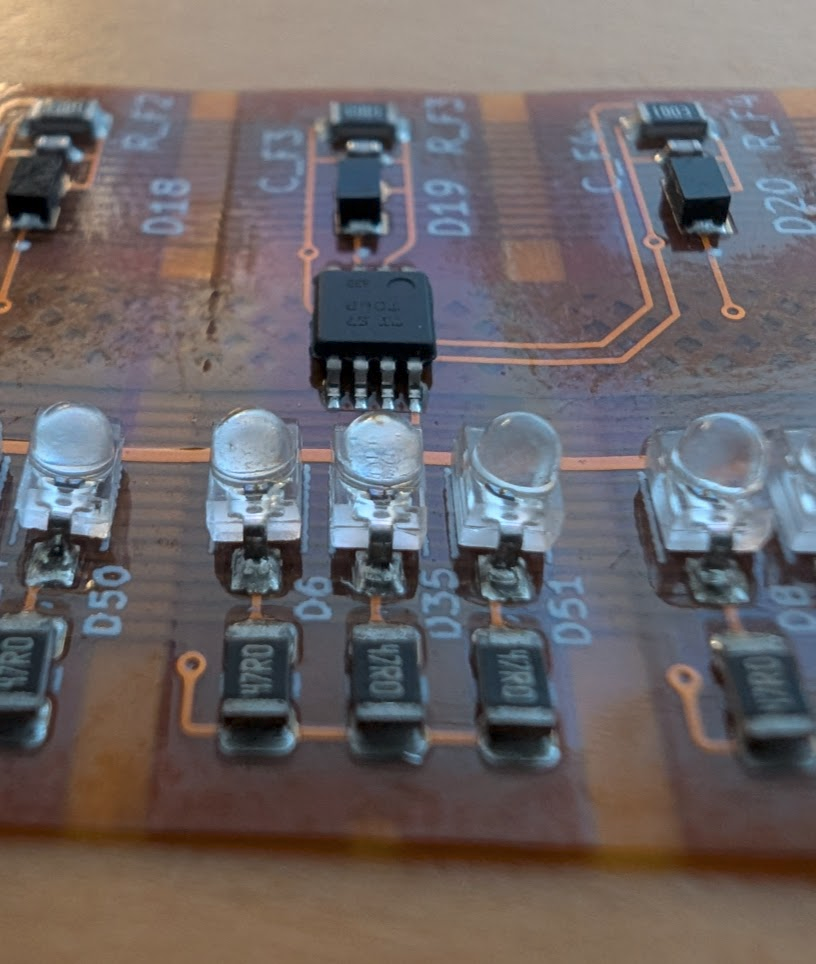
\includegraphics[width=\textwidth]{narrow_leds.png}
         \caption{$\pm 12^\circ$ LEDs}
         \label{fig:narrow_leds}
     \end{subfigure}
      \begin{subfigure}[b]{0.335\textwidth}
         \centering
         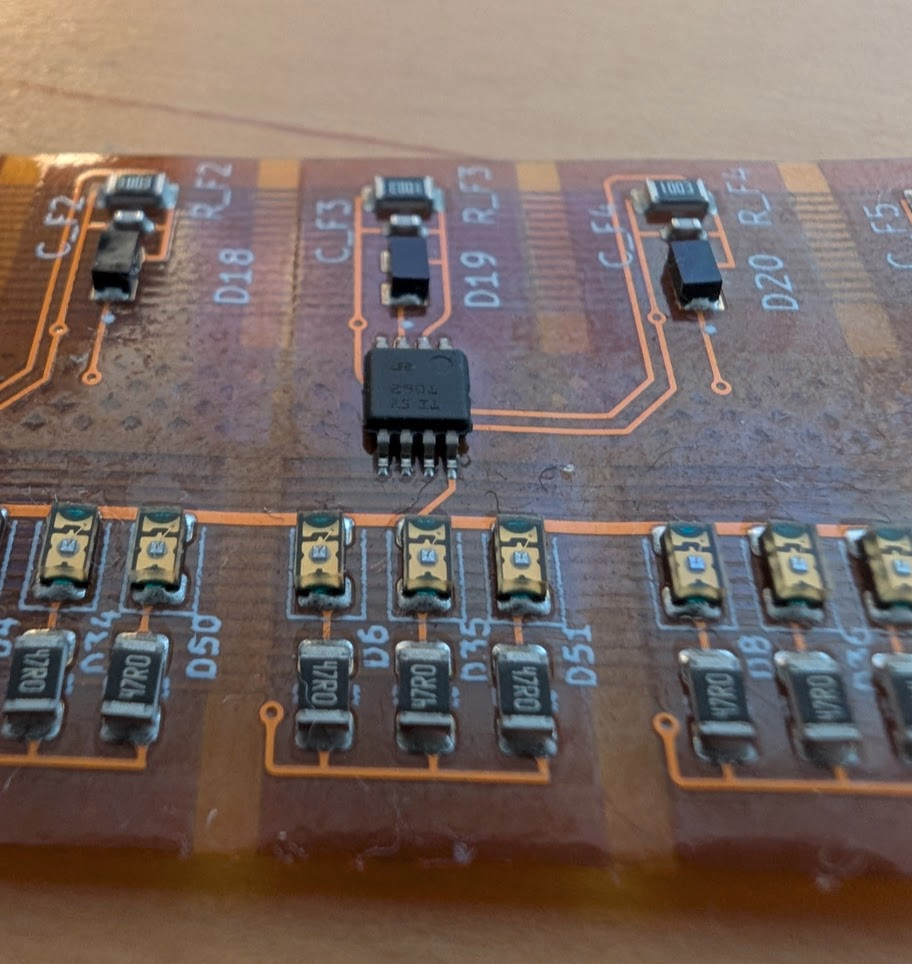
\includegraphics[width=\textwidth]{wide_leds.png}
         \caption{$\pm 60^\circ$ LEDs}
         \label{fig:wide_leds}
     \end{subfigure}
    \caption{Package sizes of the two LED types}
    \label{fig:led_types}
\end{figure}

Although the LEDs we compared were matched for radiant power and wavelength, the physical package size differs (see \autoref{fig:led_types}). This introduces a small potential confounding variable - different package sizes may slightly alter the way the LEDs couple with the skin, possibly influencing the interaction of IR light with the wrist tissue. Although the data strongly suggests that the higher radiant intensity of the $\pm 12^\circ$ LEDs produces better transmission features, we cannot entirely isolate this effect from the package size and sensor-skin coupling. However, based on FlexIR's findings that slight variations in skin coupling did not affect the accuracy, and the large magnitude of the performance difference in transmission features, this effect is considered negligible.

\section{Gesture Set}
The gesture set used to evaluate FlexIR contained a wide range hand gestures, spanning from large distinct hand and wrist positions to subtle finger movements. The most confusion came from the pinch gestures (pinch\_index, pinch\_middle, pinch\_ring and pinch\_pinkie) - for models trained on all features, pinches accounted for 43.1\% of the misclassifications on the  $\pm 12^\circ$ wristband and 41.9\% of the misclassifications on the  $\pm 60^\circ$ wristband. When trained on data excluding the pinch gestures, the model performances increased from 81.6\% to 89.0\% and 78.2\% to 86.7\% on the $\pm 12^\circ$ and $\pm 60^\circ$ wristbands respectively. This mirrors findings from GestIR and SensIR, confirming their conclusions that subtle finger movements are inherently difficult for IR sensing systems to detect.

\section{Hardware Challenges}
One of the main contributions of this project is the design and evaluation of a complex, novel flexible PCB wristband. This project used an iterative design process, shown in \autoref{section:wristband_iteration}. The main challenge when iterating on the design was the manufacturing time - we used JLCPCB to manufacture and assemble the wristbands, and the lead time between uploading schematics and receiving hardware was a major bottleneck.

The project was also plagued by hardware issues and malfunctions:

\textbf{Upside Down Components}

We used JLCPCB for PCB manufacturing and assembly, and KiCad for PCB design. Due to compatibility issues between JLCPCB and KiCad, multiple PCBs arrived with components in the wrong orientation. A significant amount of time was spent rearranging small SMD components using a hot air reflow station.

\textbf{Thin Traces}

Repeated flexing of the wristband during user studies caused some traces to break. For future iterations of the design, we recommend increasing the trace width from the current values (0.2mm).

\textbf{Manufacturing Errors}

Part way through data collection, the pair of wristbands being used broke due to repeated flexing. When we switched to the pair of backup wristbands, we identified a single op-amp with the wrong orientation. This produced a short that prevented the rest of the segments from operating. It was unfeasible to rotate the op-amp due to its small pitch, so we removed it, preventing us from reading photodiode values form segments 2 and 3. Because of this, all models are trained on 16x14 capture matrices, with the photodiode readings from segments 2 and 3 removed. This resulted in a small but consistent drop in accuracy when compared to models trained on full 16x16 capture matrices, shown in \autoref{fig:broken_segments_graph}. Because of this, we would expect a fully functioning wristband to achieve a small performance boost on all results obtained in this experiment.

Wearable devices in real world environments are highly susceptible to everyday wear and tear. The fact that FlexIR was still able to operate with two broken photodiodes, showing only a slight performance drop in one of the wristbands, demonstrates the resilience of infrared sensing systems.

\section{Theoretical Performance}
Due to the removal of two photodiode readings from the data, there was a small drop in accuracy for the $\pm 60^\circ$ wristband. On a fully functioning wristband, we would expect a performance boost of 1.69\%, resulting in an average accuracy of 79.9\%. Also, to satisfy the constraints of viewing angle and radiant power, LEDs with 940 nm wavelengths were chosen. The wavelength study conducted in GestIR \cite{diamand2025} identified 950 nm as a less effective wavelength due to the absorption peak in lipids between 930 nm and 1040 nm. 890 nm LEDs achieved a 3.4\% performance increase over 950 nm LEDs. Applying these increases to our results gives theoretical accuracies shown in \autoref{tab:theoretical_accs}.

\begin{table}[htp]
    \centering
    \begin{tabular}{lrr}
        \toprule
        Experiment & $\pm 12^\circ$ LED Accuracy & $\pm 60^\circ$ LED Accuracy \\
        \midrule
        All Features, All Gestures & 85.0\% & 83.3\% \\
        All Features, Excluding Pinch Gestures & 92.4\% & 91.8\% \\
        \bottomrule
    \end{tabular}
    \caption{Theoretical accuracy of fully functioning wristbands with 890 nm LEDs}
    \label{tab:theoretical_accs}
\end{table}

\section{Generalisation Across Sessions}
To achieve the practicality needed for everyday use, gesture recognition systems like FlexIR need to generalise well across sessions. The main difficulty is sensor misalignment due to the user wearing the wristband in slightly different positions across sessions. SensIR\cite{McIntosh2017SensIR:Reflection} gathered data from 12 different placements on the wrist and successfully determined the orientation of the wristband using a neural network regressor. In a system designed for everyday use, a calibration algorithm like this would likely be used to estimate the orientation of the device and adjust the readings accordingly.

In this project, participants collected data for each wristband in one session, without taking off or readjusting the wristband. Future investigations into the effect of LED viewing angle on the effectiveness of calibration algorithms are needed to see if the higher tissue penetration achieved with narrow angle LEDs is at the cost of more susceptibility to sensor misalignment.

\chapter{Conclusion}
\label{chap:conclusion}

\section{Project Achievements}
\noindent
This project achieved all its intended research goals.

The first major achievement is the design, manufacture, and evaluation of a new flexible PCB based gesture recognition wristband. Previous designs of similar gesture recognition systems have been useful as research platforms investigating the field of gesture recognition, but lack in practicality and reliability. FlexIRs design has multiple benefits:
\begin{itemize}
    \item Wristbands can be produced using third party PCBA services. This makes high quality hardware more easily obtainable, reducing the skill level needed to run a trial and enabling future data collection and experiments on a wider range of participants without the overhead of building wristbands by hand.
    \item The reduced form factor and improved reliability moves the device closer to a product capable of real world gesture recognition
    \item The higher density of components compared to other similar devices means that more LEDs and photodiodes can be used to produce more data
\end{itemize}

A secondary achievement of this project was a user study comparing the effectiveness of two wristbands containing LEDs with contrasting viewing angles. This yielded multiple findings:

\begin{itemize}
    \item Confirmed previous findings that traditional MLPs outperform more complex models like CNNs
    \item Results suggest that a narrow viewing angle LED with a higher peak radiant intensity generates better features from deeper tissue, although further research is required to completely isolate this from LED package size.
    \item The most crucial data for gesture recognition comes from readings with small LED - sensor distances, suggesting shallow reflections generate the best features
    \item LED viewing angle isn't a factor in how much training data models need to learn gestures
    \item IR sensing systems based only on the dorsal side of the wrist are less effective than devices surrounding the full circumference of the wrist, suggesting that future smartwatch designs should incorporate sensing hardware around the strap rather than just in the watch head.
\end{itemize}

\section{Future Work}

Although this project improves on the practicality and ergonomics of previous wristband designs, more design optimisation is needed to transition the device from a research tool into a real product.

\subsection{General PCB Optimisation}
Although the FlexIR wristband was heavily iterated to optimise practicality and functionality, there are still some improvements to be made:
\begin{itemize}
    \item Increasing the trace width would help protect them from damage due to repeated flexing
    \item Using smaller Darlington arrays and shift registers, as well as further optimising the layout of components, would reduce the form factor
\end{itemize}

\subsection{Wristband Ergonomics}
In the current design, the LEDs and photodiodes make direct contact with the wrist. Over long sessions, this becomes uncomfortable and can leave indentations in the skin. Encasing the wristband in a soft material, e.g. silicon, could improve the ergonomics. However, research is necessary into the effect of introducing additional materials between the sensing circuits and the skin.

\subsection{On-board processing}
The current design also contains no on-board processing capabilities. During use, the device is plugged into a microcontroller via an FFC cable which controls the LEDs and reads from the photodiodes. This communicates with a computer, which performs model training and inference, through a USB cable. Performing inference on the wristband would remove the need for physical tethering to a computer or microcontroller, improving practicality. There are two main challenges in achieving this:

\begin{itemize}
    \item Adding processing capability to the wristband
    \item Optimising the models for inference on embedded systems
\end{itemize}

\subsection{Larger trials}
The FlexIR wristband can be easily manufactured and assembled using third party PCBA services. This opens the door to larger user studies and machine learning experiments without the need for hardware expertise. There are lots of possible avenues for further investigation, such as:
\begin{itemize}
    \item Investigating the effect of anatomical factors such as skin tone, muscle and fat density
    \item Gathering data and generalising models over multiple sessions
\end{itemize}

Minor modifications to the wristband hardware would allow comparison of a wider range of component properties, including but not limited to:
\begin{itemize}
    \item Finer exploration of LED wavelength and viewing angle
    \item Photodiode viewing angle
    \item Transimpedance amplifier configuration 
\end{itemize}

These extensions would gain more practical insights into optimal hardware for infrared sensing and would further transition the project from a research tool to a practical wearable device.


% The concluding chapter of a dissertation is often underutilised because it 
% is too often left too close to the deadline: it is important to allocate
% enough attention to it.  Ideally, the chapter will consist of three parts:

% \begin{enumerate}
% \item (Re)summarise the main contributions and achievements, in essence
%       summing up the content.
% \item Clearly state the current project status (e.g., ``X is working, Y 
%       is not'') and evaluate what has been achieved with respect to the 
%       initial aims and objectives (e.g., ``I completed aim X outlined 
%       previously, the evidence for this is within Chapter Y'').  There 
%       is no problem including aims which were not completed, but it is 
%       important to evaluate and/or justify why this is the case.
% \item Outline any open problems or future plans.  Rather than treat this
%       only as an exercise in what you {\em could} have done given more 
%       time, try to focus on any unexplored options or interesting outcomes
%       (e.g., ``my experiment for X gave counter-intuitive results, this 
%       could be because Y and would form an interesting area for further 
%       study'' or ``users found feature Z of my software difficult to use,
%       which is obvious in hindsight but not during at design stage; to 
%       resolve this, I could clearly apply the technique of Smith [7]'').
% \end{enumerate}

% =============================================================================

% Finally, after the main matter, the back matter is specified.  This is
% typically populated with just the bibliography.  LaTeX deals with these
% in one of two ways, namely
%
% - inline, which roughly means the author specifies entries using the 
%   \bibitem macro and typesets them manually, or
% - using BiBTeX, which means entries are contained in a separate file
%   (which is essentially a databased) then inported; this is the 
%   approach used below, with the databased being dissertation.bib.
%
% Either way, the each entry has a key (or identifier) which can be used
% in the main matter to cite it, e.g., \cite{X}, \cite[Chapter 2}{Y}.
%
% We would recommend using BiBTeX, since it guarantees a consistent referencing style 
% and since many sites (such as dblp) provide references in BiBTeX format. 
% However, note that by default, BiBTeX will ignore capital letters in article titles 
% to ensure consistency of style. This can lead to e.g. "NP-completeness" becoming
% "np-completeness". To avoid this, make sure any capital letters you want to preserve
% are enclosed in braces in the .bib, e.g. "{NP}-completeness".

\backmatter

\bibliography{references, dissertation}

% -----------------------------------------------------------------------------

% The dissertation concludes with a set of (optional) appendicies; these are 
% the same as chapters in a sense, but once signaled as being appendicies via
% the associated macro, LaTeX manages them appropriatly.

\appendix

\chapter{Appendix A: AI Prompts/Tools}
\label{appx:ai_prompt}

AI has been used sparingly in this project to enable rapid iteration. Where small portions of AI generated code are used, they have been thoroughly checked and edited.

\begin{itemize}
    \item IntelliJ's code completion, which is powered by an AI assistant, was used to assist in the of the Python software.
    \item Overleaf's Writefull, which uses custom language models trained on research papers and fine-tuned to LaTeX, was used for spelling and grammar suggestions.
    \item GPT-5.2 and Gemini 3.1 Pro were used to assist in writing code to generate graphs and visualisations using matplotlib.
\end{itemize}

\chapter{Statistical Test Results}
\label{appx:stats_results}

\begin{table}[htp]
    \centering
    \begin{tabular}{lrrrr}
        \toprule
        Condition & $t$ & $p$ & $p_{adj}$ & Cohen's $d$ \\
        \midrule
        All Features, All Gestures & 1.758 & 0.109 & 0.124 & -0.530 \\
        All Features, Excluding Pinch Gestures & 1.679 & 0.124 & 0.124 & -0.506 \\
        Transmission Features (Band Width 3), All Gestures & 5.362 & 0.000 & 0.002 & -1.617 \\
        Transmission Features (Band Width 5), All Gestures & 3.709 & 0.004 & 0.012 & -1.118 \\
        Reflection Features (Band Width 3), All Gestures & 1.803 & 0.102 & 0.124 & -0.544 \\
        Smartwatch Features, All Gestures & 2.773 & 0.020 & 0.039 & -0.836 \\
        \bottomrule
    \end{tabular}
    \caption{Results of paired $t$-tests comparing the accuracies of the $\pm 12^\circ$ and $\pm 60^\circ$ wristbands when trained using different sets of features}
    \label{tab:overall_results}
\end{table}

\begin{table}[htp]
    \centering
    \begin{tabular}{lrrrr}
        \toprule
        Condition & $t$ & $p$ & $p_{adj}$ & Cohen's $d$ \\
        \midrule
        70 captures (25\% of full training set) & -1.112 & 0.292 & 0.292 & 0.335 \\
        140 captures (50\% of full training set) & -1.620 & 0.136 & 0.182 & 0.488 \\
        210 captures (75\% of full training set) & -1.887 & 0.088 & 0.182 & 0.569 \\
        280 captures (100\% of full training set) & -1.758 & 0.109 & 0.182 & 0.530 \\
        \bottomrule
    \end{tabular}
    \caption{Results of paired $t$-tests comparing the accuracies of the $\pm 12^\circ$ and $\pm 60^\circ$ wristbands when trained on varying training set sizes}
    \label{tab:training_set_results}
\end{table}

\begin{table}[htp]
    \centering
    \begin{tabular}{lrrrr}
        \toprule
        Condition & $t$ & $p$ & $p_{adj}$ & Cohen's $d$ \\
        \midrule
        Reflection Features (Band Width 3), All Gestures & -0.461 & 0.655 & 0.727 & 0.139 \\
        Transmission Features (Band Width 3), All Gestures & 8.609 & 0.000 & 0.000 & -2.596 \\
        Transmission Features (Band Width 5), All Gestures & 21.449 & 0.000 & 0.000 & -6.467 \\
        Smartwatch Features, All Gestures & 10.937 & 0.000 & 0.000 & -3.298 \\
        All Features, Excluding Broken Gestures, All Gestures & -2.062 & 0.094 & 0.118 & 0.842 \\
        \bottomrule
    \end{tabular}
    \caption{Results of paired $t$-tests comparing the performance of models trained on different features to the performance of models trained on all features for the $\pm 12^\circ$ wristband}
    \label{tab:training_set_results_12}
\end{table}

\begin{table}[htp]
    \centering
    \begin{tabular}{lrrrr}
        \toprule
        Condition & $t$ & $p$ & $p_{adj}$ & Cohen's $d$ \\
        \midrule
        Reflection Features (Band Width 3), All Gestures & -0.244 & 0.812 & 0.812 & 0.074 \\
        Transmission Features (Band Width 3), All Gestures & 15.284 & 0.000 & 0.000 & -4.608 \\
        Transmission Features (Band Width 5), All Gestures & 25.373 & 0.000 & 0.000 & -7.650 \\
        Smartwatch Features, All Gestures & 10.474 & 0.000 & 0.000 & -3.158 \\
        All Features, Excluding Broken Gestures, All Gestures & -2.966 & 0.031 & 0.045 & 1.211 \\
        \bottomrule
    \end{tabular}
    \caption{Results of paired $t$-tests comparing the performance of models trained on different features to the performance of models trained on all features for the $\pm 60^\circ$ wristband}
    \label{tab:training_set_results_60}
\end{table}

\begin{table}[htp]
    \centering
    \begin{tabular}{lrrrr}
        \toprule
        Experiment & $t$ & $p$ & $p_{adj}$ & Cohen's $d$ \\
        \midrule
        All Features, All Gestures & 2.136 & 0.063 & 0.291 & 1.300 \\
        All Features, Excluding Pinch Gestures & 0.953 & 0.369 & 0.369 & 0.546 \\
        Transmission Features (Band Width 3), All Gestures & 1.272 & 0.237 & 0.291 & 0.737 \\
        Transmission Features (Band Width 5), All Gestures & 1.358 & 0.218 & 0.291 & 0.765 \\
        Reflection Features (Band Width 3), All Gestures & 1.586 & 0.152 & 0.291 & 0.979 \\
        Smartwatch Features, All Gestures & 1.259 & 0.242 & 0.291 & 0.727 \\
        \bottomrule
    \end{tabular}
    \caption{Results of unpaired $t$-tests to investigative order effects}
    \label{tab:order_effects}
\end{table}

\begin{table}[htp]
    \centering
    \begin{tabular}{lrrr}
        \toprule
        Experiment & $H$ & $p$ & $p_{adj}$ \\
        \midrule
        All Features, All Gestures & 0.000 & 1.000 & 1.000 \\
        All Features, Excluding Pinch Gestures & 2.006 & 0.432 & 0.741 \\
        Transmission Features (Band Width 3), All Gestures & 0.240 & 0.895 & 0.976 \\
        Transmission Features (Band Width 5), All Gestures & 3.461 & 0.202 & 0.646 \\
        Reflection Features (Band Width 3), All Gestures & 0.526 & 0.807 & 0.976 \\
        Smartwatch Features, All Gestures & 1.597 & 0.509 & 0.764 \\
        \bottomrule
    \end{tabular}
    \caption{Results of permutation tests to investigate environmental effects for the $\pm 12^\circ$ wristband}
    \label{tab:location_effects_12}
\end{table}

\begin{table}[htp]
    \centering
    \begin{tabular}{lrrr}
        \toprule
        Experiment & $H$ & $p$ & $p_{adj}$ \\
        \midrule
        All Features, All Gestures & 2.734 & 0.323 & 0.646 \\
        All Features, Excluding Pinch Gestures & 3.591 & 0.182 & 0.646 \\
        Transmission Features (Band Width 3), All Gestures & 3.273 & 0.218 & 0.646 \\
        Transmission Features (Band Width 5), All Gestures & 5.435 & 0.034 & 0.412 \\
        Reflection Features (Band Width 3), All Gestures & 2.740 & 0.311 & 0.646 \\
        Smartwatch Features, All Gestures & 0.344 & 0.869 & 0.976 \\
        \bottomrule
    \end{tabular}
    \caption{Results of permutation tests to investigate environmental effects for the $\pm 60^\circ$ wristband}
    \label{tab:location_effects_60}
\end{table}

\begin{table}[htp]
    \centering
    \begin{tabular}{lrrr}
        \toprule
        Condition & $r$ & $p$ & $p_{adj}$ \\
        \midrule
        All Features, All Gestures & -0.112 & 0.743 & 0.999 \\
        All Features, Excluding Pinch Gestures & -0.007 & 0.983 & 0.999 \\
        Transmission Features (Band Width 3), All Gestures & -0.160 & 0.638 & 0.999 \\
        Transmission Features (Band Width 5), All Gestures & 0.000 & 0.999 & 0.999 \\
        Reflection Features (Band Width 3), All Gestures & -0.193 & 0.569 & 0.999 \\
        Smartwatch Features, All Gestures & -0.011 & 0.975 & 0.999 \\
        \bottomrule
    \end{tabular}
    \caption{Results of Pearson correlation tests between model performance and participant wrist circumference for the $\pm 12^\circ$ wristband}
    \label{tab:correlation_12}
\end{table}

\begin{table}[htp]
    \centering
    \begin{tabular}{lrrr}
        \toprule
        Condition & $r$ & $p$ & $p_{adj}$ \\
        \midrule
        All Features, All Gestures & 0.056 & 0.869 & 0.999 \\
        All Features, Excluding Pinch Gestures & 0.141 & 0.679 & 0.999 \\
        Transmission Features (Band Width 3), All Gestures & -0.259 & 0.442 & 0.999 \\
        Transmission Features (Band Width 5), All Gestures & -0.069 & 0.840 & 0.999 \\
        Reflection Features (Band Width 3), All Gestures & 0.089 & 0.794 & 0.999 \\
        Smartwatch Features, All Gestures & -0.114 & 0.738 & 0.999 \\
        \bottomrule
    \end{tabular}
    \caption{Results of Pearson correlation tests between model performance and participant wrist circumference for the $\pm 60^\circ$ wristband}
    \label{tab:correlation_60}
\end{table}

\chapter{Confusion Matrices}
\label{appx:cms}

\begin{figure}[htp]
     \centering
     \begin{subfigure}[b]{0.8\textwidth}
         \centering
         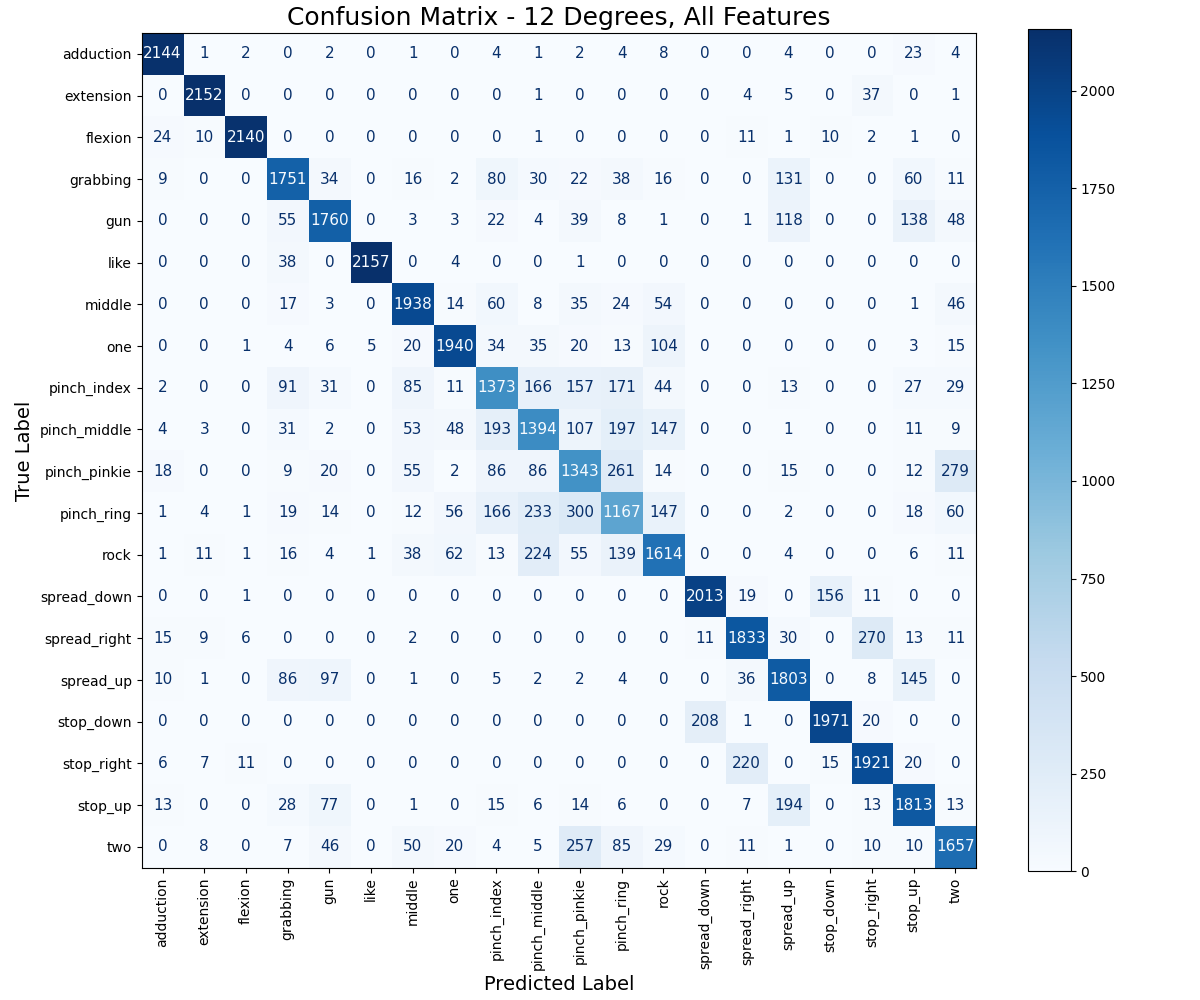
\includegraphics[width=\textwidth]{figures/cm_12_degrees_all.png}
         \caption{$\pm 12^\circ$ wristband}
         \label{fig:cm_all_12}
     \end{subfigure}
      \begin{subfigure}[b]{0.8\textwidth}
         \centering
         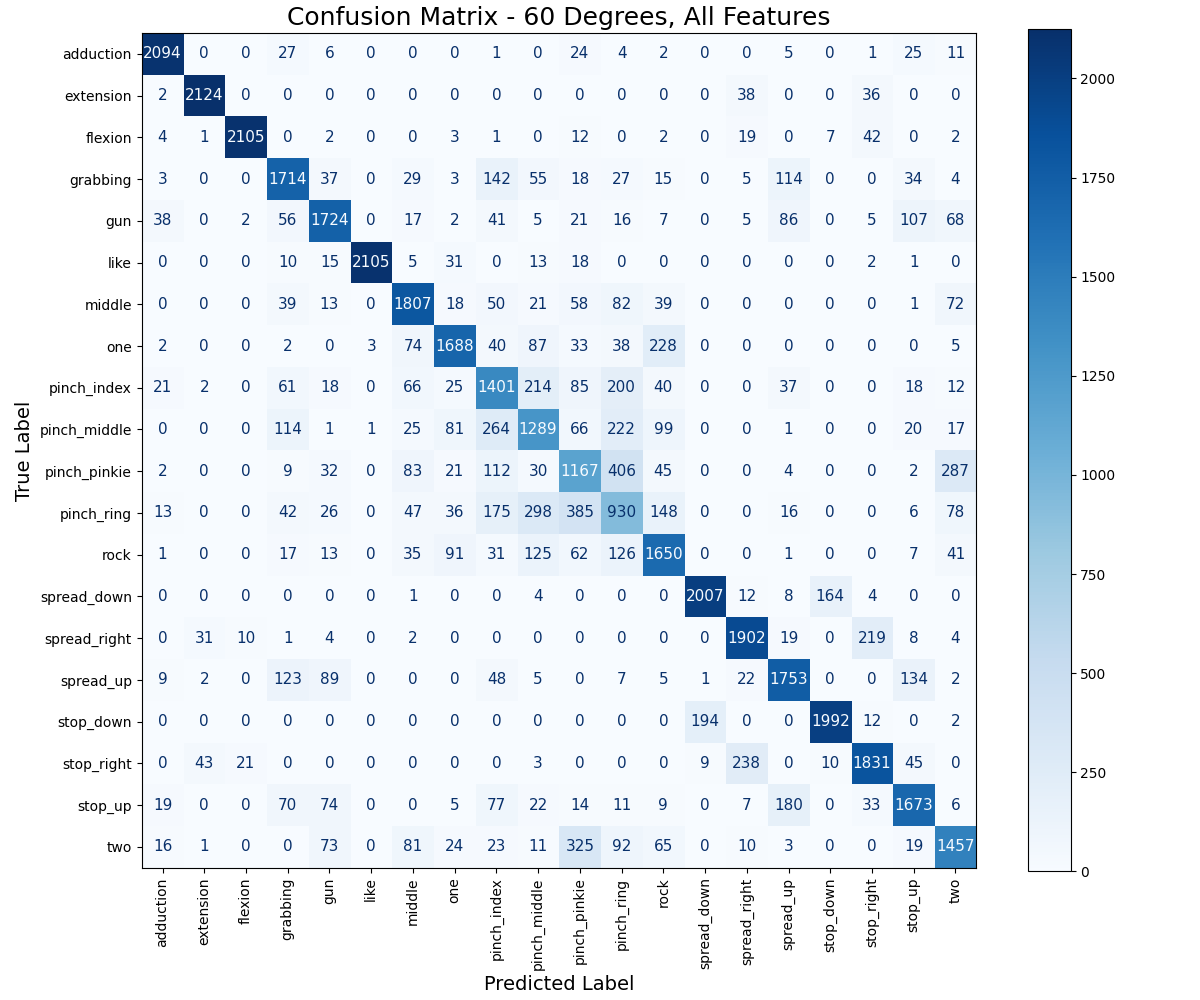
\includegraphics[width=\textwidth]{figures/cm_60_degrees_all.png}
         \caption{$\pm 60^\circ$ wristband}
         \label{fig:cm_all_60}
     \end{subfigure}
    \caption{Confusion matrices for MLPs with Monte Carlo Dropout trained on all features aggregated over all participants}
    \label{fig:cm_all}
\end{figure}

\begin{figure}[htp]
     \centering
     \begin{subfigure}[b]{0.8\textwidth}
         \centering
         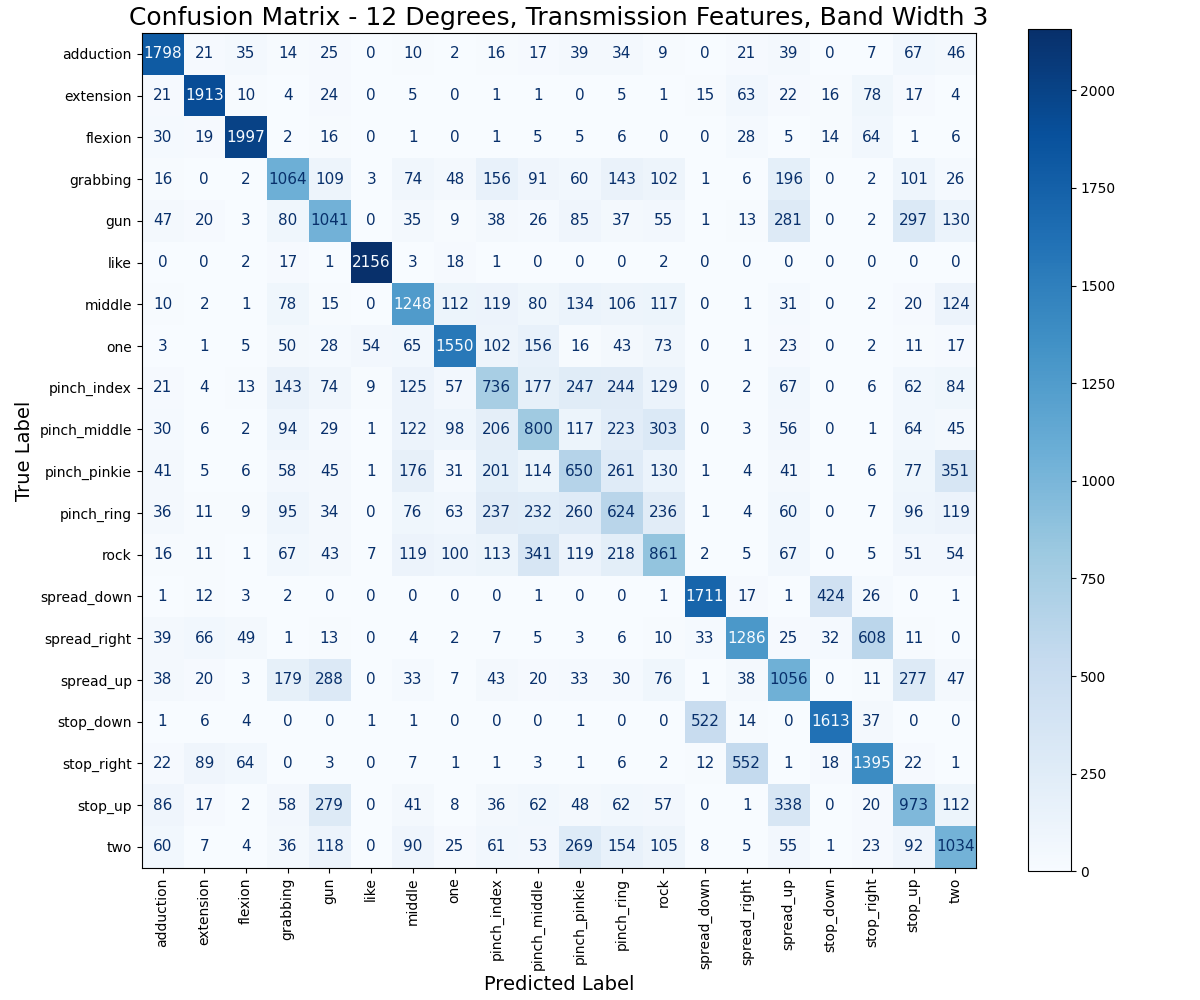
\includegraphics[width=\textwidth]{figures/cm_12_degrees_transmission_3.png}
         \caption{$\pm 12^\circ$ wristband}
         \label{fig:cm_t3_12}
     \end{subfigure}
      \begin{subfigure}[b]{0.8\textwidth}
         \centering
         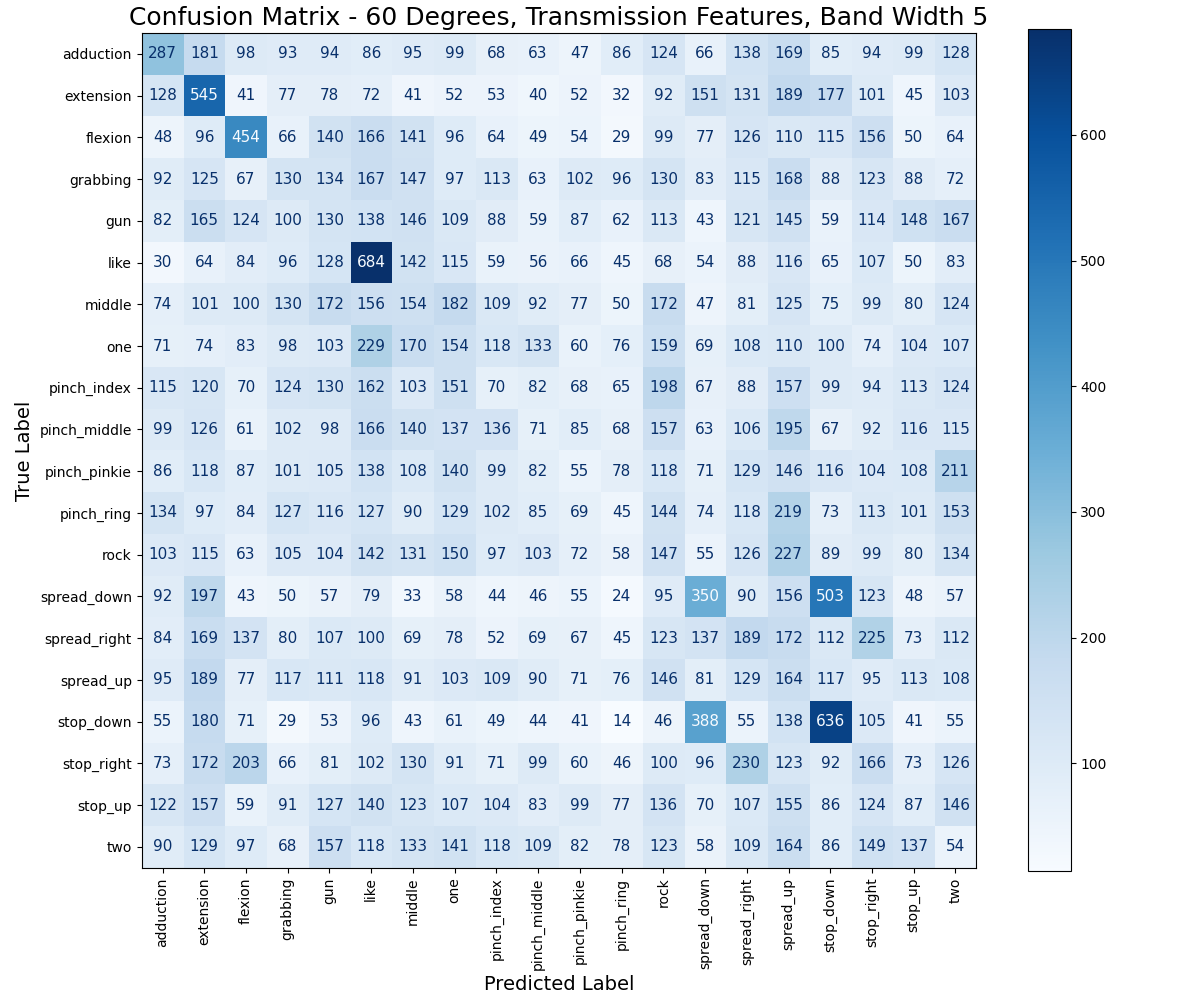
\includegraphics[width=\textwidth]{figures/cm_60_degrees_transmission_5.png}
         \caption{$\pm 60^\circ$ wristband}
         \label{fig:cm_t3_60}
     \end{subfigure}
    \caption{Confusion matrices for MLPs with Monte Carlo Dropout trained on transmission features with band width 3, aggregated over all participants}
    \label{fig:samples_transmission_3}
\end{figure}

\begin{figure}[htp]
     \centering
     \begin{subfigure}[b]{0.8\textwidth}
         \centering
         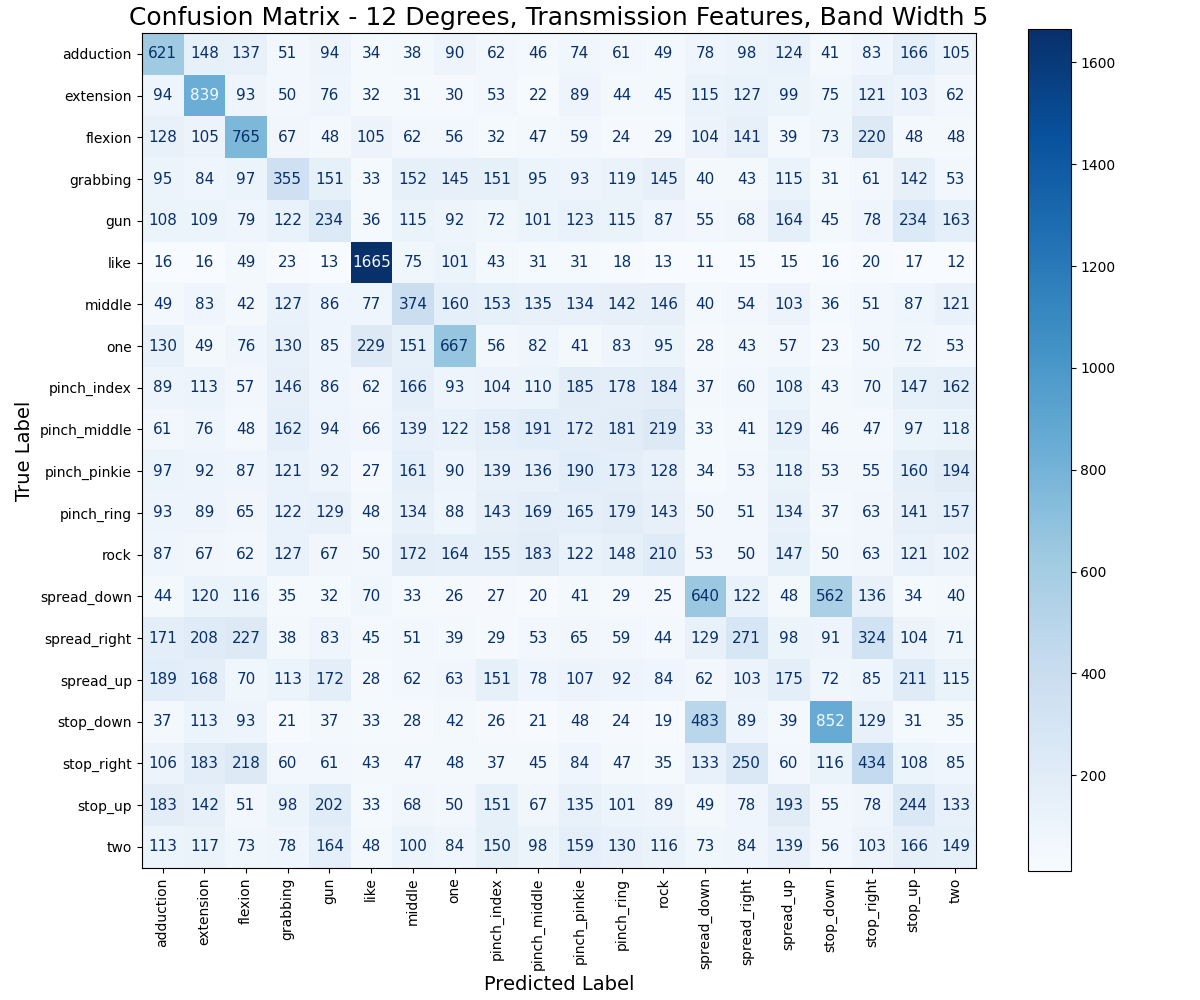
\includegraphics[width=\textwidth]{figures/cm_12_degrees_transmission_5.png}
         \caption{$\pm 12^\circ$ wristband}
         \label{fig:cm_t5_12}
     \end{subfigure}
      \begin{subfigure}[b]{0.8\textwidth}
         \centering
         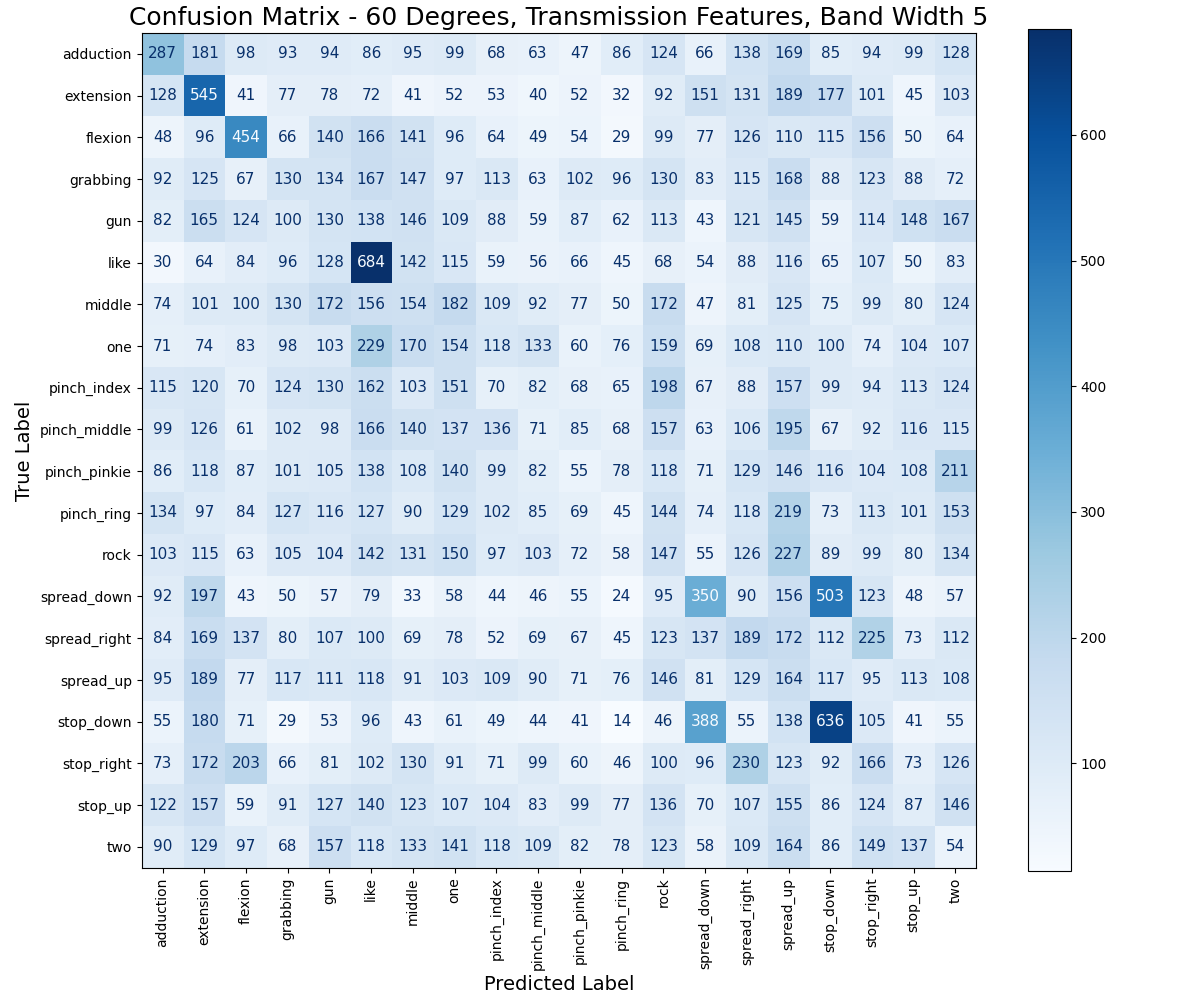
\includegraphics[width=\textwidth]{figures/cm_60_degrees_transmission_5.png}
         \caption{$\pm 60^\circ$ wristband}
         \label{fig:cm_t5_60}
     \end{subfigure}
    \caption{Confusion matrices for MLPs with Monte Carlo Dropout trained on transmission features with band width 5, aggregated over all participants}
    \label{fig:samples_transmission_5}
\end{figure}

\begin{figure}[htp]
     \centering
     \begin{subfigure}[b]{0.8\textwidth}
         \centering
         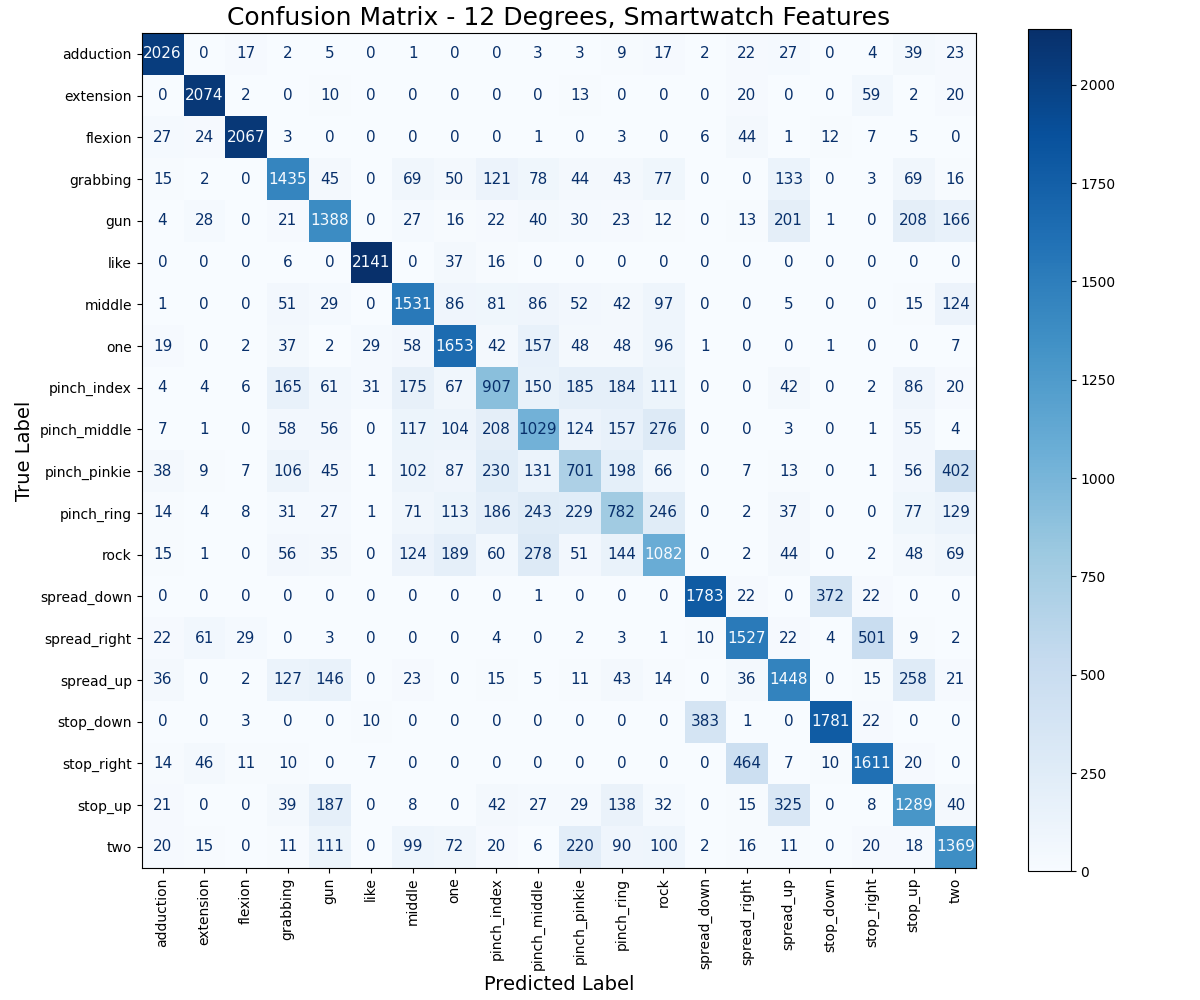
\includegraphics[width=\textwidth]{figures/cm_12_degrees_smartwatch.png}
         \caption{$\pm 12^\circ$ wristband}
         \label{fig:cm_smartwatch_1}
     \end{subfigure}
      \begin{subfigure}[b]{0.8\textwidth}
         \centering
         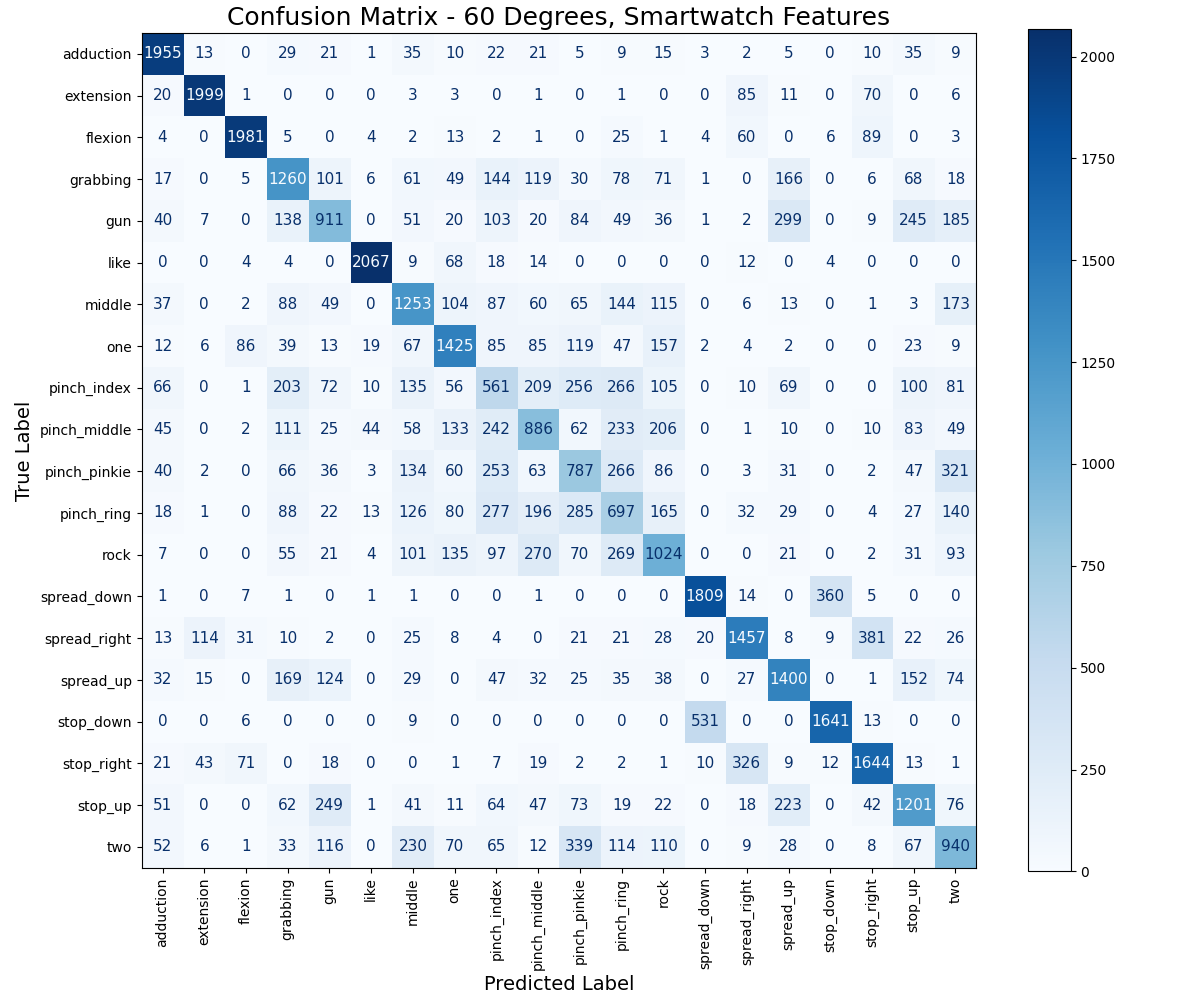
\includegraphics[width=\textwidth]{figures/cm_60_degrees_smartwatch.png}
         \caption{$\pm 60^\circ$ wristband}
         \label{fig:cm_smartwatch_2}
     \end{subfigure}
    \caption{Confusion matrices for MLPs with Monte Carlo Dropout trained on smartwatch features (segments 8, 9, 10, and 11), aggregated over all participants}
    \label{fig:cm_smartwatch}
\end{figure}

\chapter{Accuracy vs Training Set Size}
\label{appx:samples}

\begin{figure}[htp]
     \centering
     \begin{subfigure}[b]{0.45\textwidth}
         \centering
         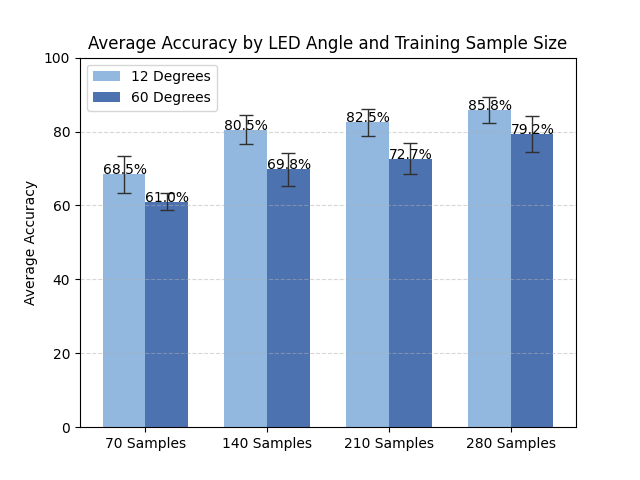
\includegraphics[width=\textwidth]{figures/sample_size_comparison_1.png}
         \caption{Participant 1}
         \label{fig:samples_all_1}
     \end{subfigure}
     \begin{subfigure}[b]{0.45\textwidth}
         \centering
         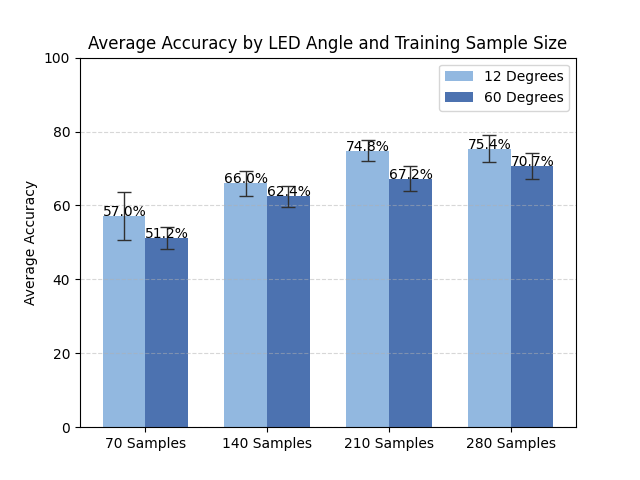
\includegraphics[width=\textwidth]{figures/sample_size_comparison_2.png}
         \caption{Participant 2}
         \label{fig:samples_all_2}
     \end{subfigure}
     \begin{subfigure}[b]{0.45\textwidth}
         \centering
         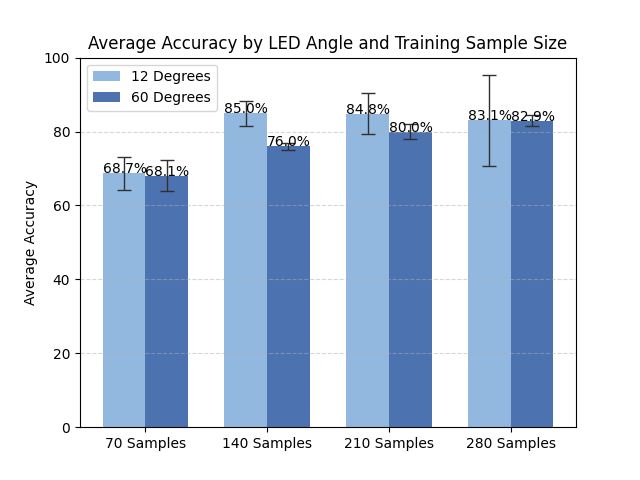
\includegraphics[width=\textwidth]{figures/sample_size_comparison_3.png}
         \caption{Participant 3}
         \label{fig:samples_all_3}
     \end{subfigure}
     \begin{subfigure}[b]{0.45\textwidth}
         \centering
         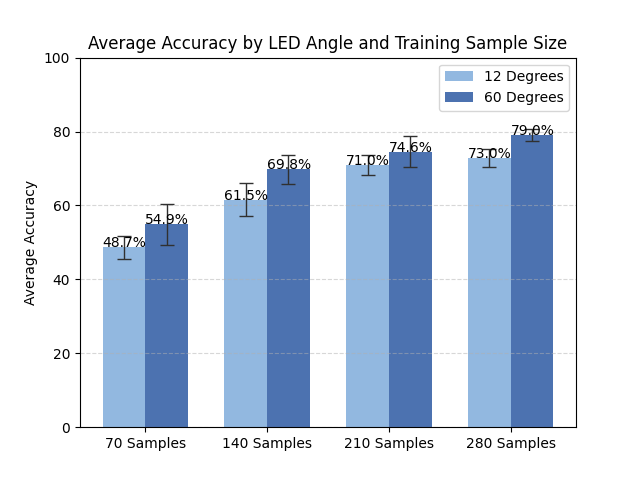
\includegraphics[width=\textwidth]{figures/sample_size_comparison_4.png}
         \caption{Participant 4}
         \label{fig:samples_all_4}
     \end{subfigure}
     \begin{subfigure}[b]{0.45\textwidth}
         \centering
         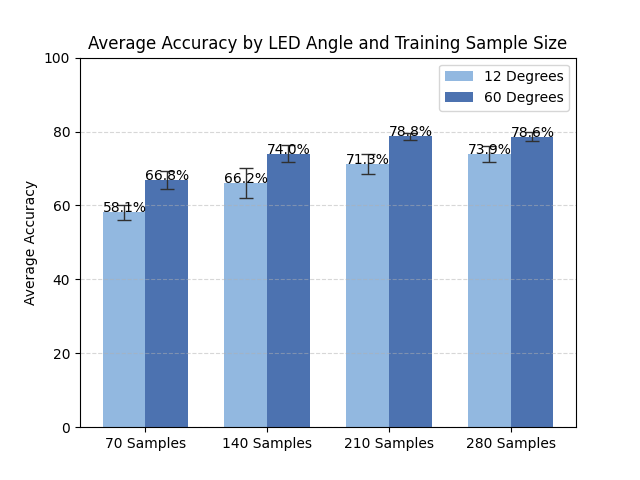
\includegraphics[width=\textwidth]{figures/sample_size_comparison_5.png}
         \caption{Participant 5}
         \label{fig:samples_all_5}
     \end{subfigure}
     \begin{subfigure}[b]{0.45\textwidth}
         \centering
         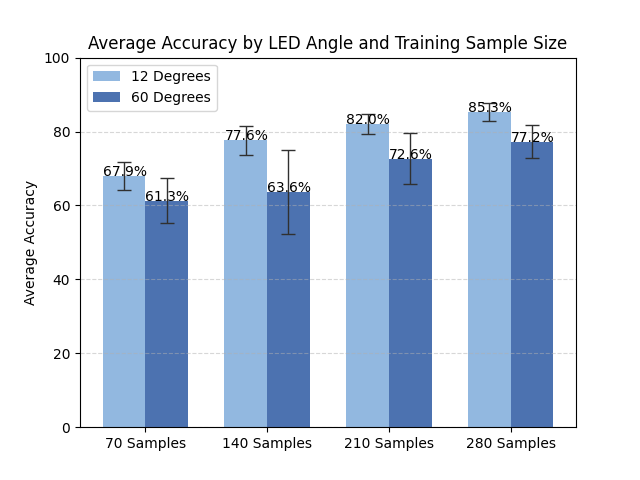
\includegraphics[width=\textwidth]{figures/sample_size_comparison_6.png}
         \caption{Participant 6}
         \label{fig:samples_all_6}
     \end{subfigure}
     \caption{Average model accuracy vs size of training set}
    \label{fig:samples_test_all}
\end{figure}

\begin{figure}[htp]
    \ContinuedFloat %
     \centering
     \begin{subfigure}[b]{0.45\textwidth}
         \centering
         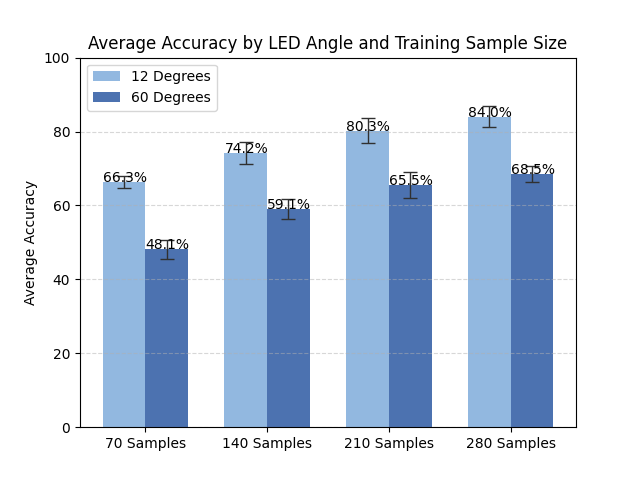
\includegraphics[width=\textwidth]{figures/sample_size_comparison_7.png}
         \caption{Participant 7}
         \label{fig:samples_all_7}
     \end{subfigure}
     \begin{subfigure}[b]{0.45\textwidth}
         \centering
         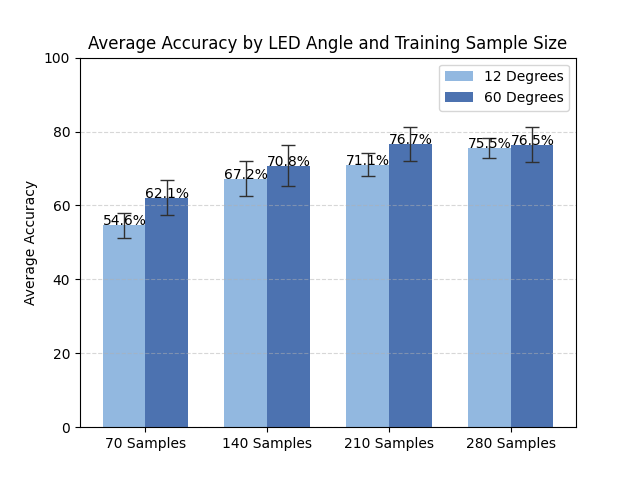
\includegraphics[width=\textwidth]{figures/sample_size_comparison_8.png}
         \caption{Participant 8}
         \label{fig:samples_all_8}
     \end{subfigure}
     \begin{subfigure}[b]{0.45\textwidth}
         \centering
         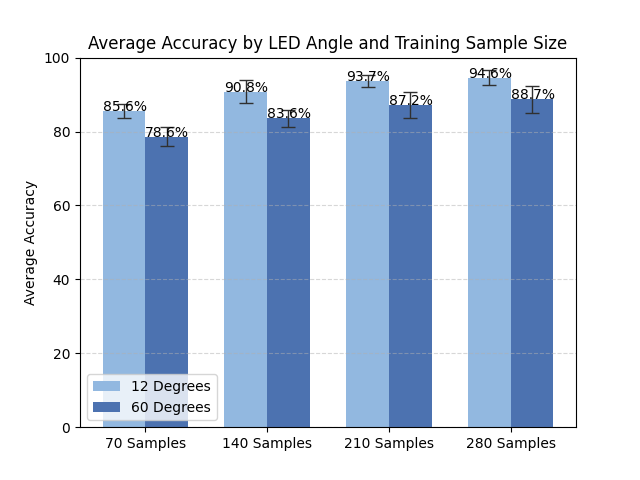
\includegraphics[width=\textwidth]{figures/sample_size_comparison_9.png}
         \caption{Participant 9}
         \label{fig:samples_all_9}
     \end{subfigure}
     \begin{subfigure}[b]{0.45\textwidth}
         \centering
         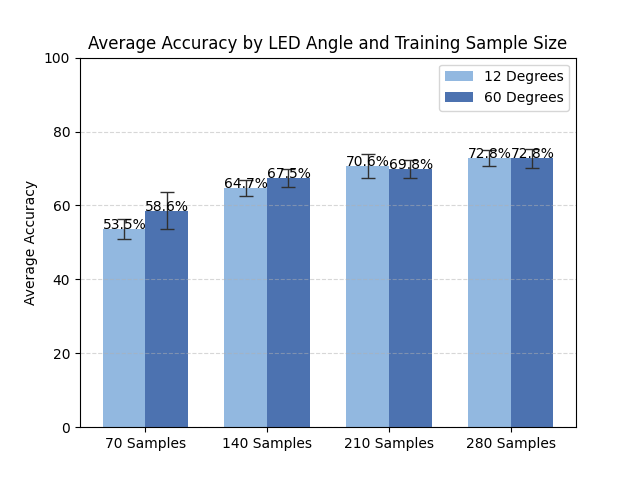
\includegraphics[width=\textwidth]{figures/sample_size_comparison_10.png}
         \caption{Participant 10}
         \label{fig:samples_all_10}
     \end{subfigure}
     \begin{subfigure}[b]{0.45\textwidth}
         \centering
         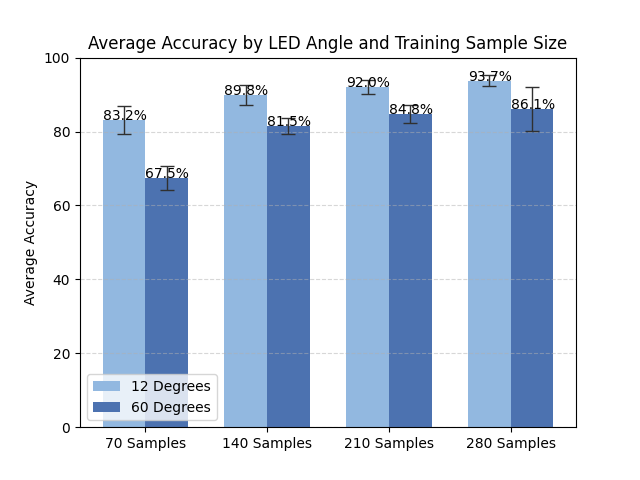
\includegraphics[width=\textwidth]{figures/sample_size_comparison_11.png}
         \caption{Participant 11}
         \label{fig:samples_all_11}
     \end{subfigure}
    \caption{Average model accuracy vs size of training set (Continued)}
\end{figure}

\chapter{Accuracy vs Wrist Circumference}
\label{appx:acc_vs_wrist_size}

\begin{figure}[htp]
     \centering
     \begin{subfigure}[b]{0.45\textwidth}
         \centering
         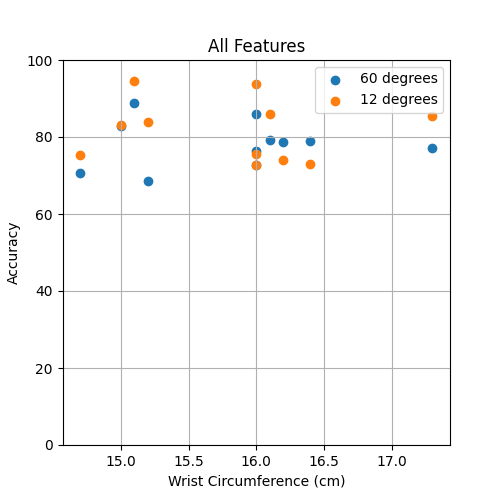
\includegraphics[width=\textwidth]{figures/accuracy_vs_wrist_size_all.png}
         \caption{All features}
         \label{fig:acc_vs_size_all}
     \end{subfigure}
     \begin{subfigure}[b]{0.45\textwidth}
         \centering
         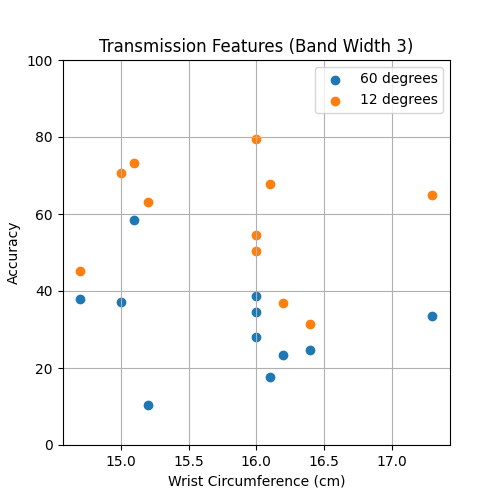
\includegraphics[width=\textwidth]{figures/accuracy_vs_wrist_size_transmission_3.png}
         \caption{Transmission features, band width 3}
         \label{fig:acc_vs_size_t3}
     \end{subfigure}
     \begin{subfigure}[b]{0.45\textwidth}
         \centering
         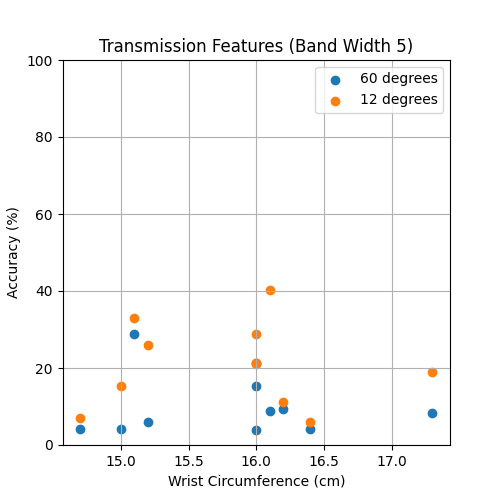
\includegraphics[width=\textwidth]{figures/accuracy_vs_wrist_size_transmission_5.png}
         \caption{Transmission features, band width 5}
         \label{fig:acc_vs_size_t5}
     \end{subfigure}
     \begin{subfigure}[b]{0.45\textwidth}
         \centering
         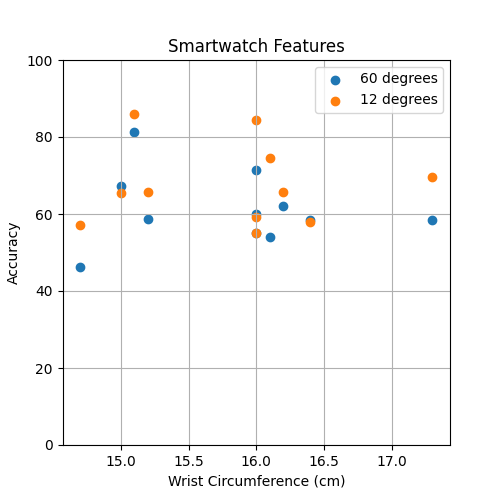
\includegraphics[width=\textwidth]{figures/accuracy_vs_wrist_size_smartwatch.png}
         \caption{Smartwatch features (segments 8, 9, 10, and 11)}
         \label{fig:acc_vs_size_smartwatch}
     \end{subfigure}
    \caption{Scatter plots showing the average model accuracy vs wrist circumference for all participants.}
    \label{fig:acc_vs_size}
\end{figure}


\end{document}